\documentclass[conference]{IEEEtran}
\IEEEoverridecommandlockouts
% Document Class: IEEEtran 2015/08/26 V1.8b by Michael Shell
% -- http://www.michaelshell.org/tex/ieeetran/

\usepackage{cite}
\usepackage{amsmath,amssymb,amsfonts}
\usepackage{algorithmic}
\usepackage{graphicx}
\usepackage{textcomp}
\usepackage{xcolor}
\usepackage{float}
\usepackage{filecontents}
\usepackage{kotex}
\usepackage{lipsum}
\usepackage{soul}

\usepackage{wrapfig}
\usepackage{makecell}
\usepackage{tabularx}
\usepackage{supertabular,booktabs}
\def\BibTeX{{\rm B\kern-.05em{\sc i\kern-.025em b}\kern-.08em
    T\kern-.1667em\lower.7ex\hbox{E}\kern-.125emX}}

\documentclass{scrreprt}
\makeatletter
\usepackage{color}
\definecolor{lightgray}{rgb}{0.95, 0.95, 0.95}
\definecolor{darkgray}{rgb}{0.4, 0.4, 0.4}
%\definecolor{purple}{rgb}{0.65, 0.12, 0.82}
\definecolor{editorGray}{rgb}{0.95, 0.95, 0.95}
\definecolor{editorOcher}{rgb}{1, 0.5, 0} % #FF7F00 -> rgb(239, 169, 0)
\definecolor{editorGreen}{rgb}{0, 0.5, 0} % #007C00 -> rgb(0, 124, 0)
\definecolor{orange}{rgb}{1,0.45,0.13}		
\definecolor{olive}{rgb}{0.17,0.59,0.20}
\definecolor{brown}{rgb}{0.69,0.31,0.31}
\definecolor{purple}{rgb}{0.38,0.18,0.81}
\definecolor{lightblue}{rgb}{0.1,0.57,0.7}
\definecolor{lightred}{rgb}{1,0.4,0.5}
\usepackage{upquote}
\usepackage{listings}
% CSS
\lstdefinelanguage{CSS}{
  keywords={color,background-image:,margin,padding,font,weight,display,position,top,left,right,bottom,list,style,border,size,white,space,min,width, transition:, transform:, transition-property, transition-duration, transition-timing-function},	
  sensitive=true,
  morecomment=[l]{//},
  morecomment=[s]{/*}{*/},
  morestring=[b]',
  morestring=[b]",
  alsoletter={:},
  alsodigit={-}
}

% JavaScript
\lstdefinelanguage{JavaScript}{
  morekeywords={typeof, new, true, false, catch, function, return, null, catch, switch, var, if, in, while, do, else, case, break},
  morecomment=[s]{/*}{*/},
  morecomment=[l]//,
  morestring=[b]",
  morestring=[b]'
}

\lstdefinelanguage{HTML5}{
  language=html,
  sensitive=true,	
  alsoletter={<>=-},	
  morecomment=[s]{<!-}{-->},
  tag=[s],
  otherkeywords={
  % General
  >,
  % Standard tags
	<!DOCTYPE,
  </html, <html, <head, <title, </title, <style, </style, <link, </head, <meta, />,
	% body
	</body, <body,
	% Divs
	</div, <div, </div>, 
	% Paragraphs
	</p, <p, </p>,
	% scripts
	</script, <script,
  % More tags...
  <canvas, /canvas>, <svg, <rect, <animateTransform, </rect>, </svg>, <video, <source, <iframe, </iframe>, </video>, <image, </image>, <header, </header, <article, </article
  },
  ndkeywords={
  % General
  =,
  % HTML attributes
  charset=, src=, id=, width=, height=, style=, type=, rel=, href=,
  % SVG attributes
  fill=, attributeName=, begin=, dur=, from=, to=, poster=, controls=, x=, y=, repeatCount=, xlink:href=,
  % properties
  margin:, padding:, background-image:, border:, top:, left:, position:, width:, height:, margin-top:, margin-bottom:, font-size:, line-height:,
	% CSS3 properties
  transform:, -moz-transform:, -webkit-transform:,
  animation:, -webkit-animation:,
  transition:,  transition-duration:, transition-property:, transition-timing-function:,
  }
}

\lstdefinestyle{htmlcssjs} {%
  % General design
%  backgroundcolor=\color{editorGray},
  basicstyle={\footnotesize\ttfamily},   
  frame=b,
  % line-numbers
  xleftmargin={0.75cm},
  numbers=left,
  stepnumber=1,
  firstnumber=1,
  numberfirstline=true,	
  % Code design
  identifierstyle=\color{black},
  keywordstyle=\color{blue}\bfseries,
  ndkeywordstyle=\color{editorGreen}\bfseries,
  stringstyle=\color{editorOcher}\ttfamily,
  commentstyle=\color{brown}\ttfamily,
  % Code
  language=HTML5,
  alsolanguage=JavaScript,
  alsodigit={.:;},	
  tabsize=2,
  showtabs=false,
  showspaces=false,
  showstringspaces=false,
  extendedchars=true,
  breaklines=true,
  % German umlauts
  literate=%
  {Ö}{{\"O}}1
  {Ä}{{\"A}}1
  {Ü}{{\"U}}1
  {ß}{{\ss}}1
  {ü}{{\"u}}1
  {ä}{{\"a}}1
  {ö}{{\"o}}1
}
%
\lstdefinestyle{py} {%
language=python,
literate=%
*{0}{{{\color{lightred}0}}}1
{1}{{{\color{lightred}1}}}1
{2}{{{\color{lightred}2}}}1
{3}{{{\color{lightred}3}}}1
{4}{{{\color{lightred}4}}}1
{5}{{{\color{lightred}5}}}1
{6}{{{\color{lightred}6}}}1
{7}{{{\color{lightred}7}}}1
{8}{{{\color{lightred}8}}}1
{9}{{{\color{lightred}9}}}1,
basicstyle=\footnotesize\ttfamily, % Standardschrift
numbers=left,               % Ort der Zeilennummern
%numberstyle=\tiny,          % Stil der Zeilennummern
%stepnumber=2,               % Abstand zwischen den Zeilennummern
numbersep=5pt,              % Abstand der Nummern zum Text
tabsize=4,                  % Groesse von Tabs
extendedchars=true,         %
breaklines=true,            % Zeilen werden Umgebrochen
keywordstyle=\color{blue}\bfseries,
frame=b,
commentstyle=\color{brown}\itshape,
stringstyle=\color{editorOcher}\ttfamily, % Farbe der String
showspaces=false,           % Leerzeichen anzeigen ?
showtabs=false,             % Tabs anzeigen ?
xleftmargin=17pt,
framexleftmargin=17pt,
framexrightmargin=5pt,
framexbottommargin=4pt,
%backgroundcolor=\color{lightgray},
showstringspaces=false,      % Leerzeichen in Strings anzeigen ?
}%
%
\makeatother

\begin{document}

\title{MulMeokNyang\\
{\footnotesize \textsuperscript{}Intelligent cat watering machine that Recognizes individual cats with AI}
}

\author{\IEEEauthorblockN{Ann Jukyung}
\IEEEauthorblockA{\textit{Dept. Information Systems} \\
\textit{Hanyang University}\\
Seoul, South Korea \\
hyoju8618@naver.com}
\and
\IEEEauthorblockN{Choi Chansol}
\IEEEauthorblockA{\textit{Dept. Information Systems} \\
\textit{Hanyang University}\\
Seoul, South Korea \\
hjk9216@naver.com}
\and
\IEEEauthorblockN{Lee Yunsun}
\IEEEauthorblockA{\textit{Dept. Film and Theatre} \\
\textit{Hanyang University}\\
Seoul, South Korea \\
justina7182@gmail.com}
\and
\IEEEauthorblockN{Hong JunGgi}
\IEEEauthorblockA{\textit{Dept. Information Systems} \\
\textit{Hanyang University}\\
Seoul, South Korea \\
sentorino@hanyang.ac.kr}
}

\maketitle

\begin{abstract}
Cats are known for their discerning palates and can be quite selective, particularly when it comes to wet food, especially if they haven't been exposed to a variety of flavors previously. This dietary preference, coupled with a reluctance to consume adequate water, can lead to dehydration and pose a significant threat to feline health. To address this issue, smart cat water dispensing systems aim to offer a solution through the identification and in-depth analysis of individual cats' unique preferences and hydration needs.
\end{abstract}

\begin{IEEEkeywords}
identification, detection, classification, opencv, cats
\end{IEEEkeywords}

\section{Role Assignment}
Roles are assigned to improve software development process and increase team productivity. Group name is called Nyangporter.
\newline

% add description if needed
\begin{table}[!htbp]\normalsize
\begin{center}
\begin{tabular}{|p{1.2cm}|p{1.9cm}|p{4.5cm}|}
\hline
\textbf{Name} & \textbf{\textit{Role}}& \textbf{\textit{Responsibilities}}\\
\hline
Choi Chansol & Development manager &
The role involves task allocation, project progression assessment, translating requirements into practical functionality, and discerning the most suitable frameworks for the project.\newline 
\newline This position also encompasses the execution of software features and active collaboration with co-workning Software Developers to deliver essential functionalities.
\\ \hline
\end{tabular}
\label{tab1}
\end{center}
\end{table}
\newpage
\begin{table}[!htbp]\normalsize
\begin{center}
\begin{tabular}{|p{1.2cm}|p{1.9cm}|p{4.5cm}|}
\hline
Ann Jukyung & Software developer &
This role primarily involves implementing software features and collaborating with fellow developers to meet feature requirements. Additionally, it includes the vital task of ensuring that the minimum viable product remains on schedule. \newline
\newline This position is also responsible for engaging with users and customers to gather and integrate feedback into the product's development process. Code maintenance and overseeing the coordination of pull requests are also integral aspects of this role.
\\ \hline
Lee Yunsun & User &
Tasked with app testing and identifying any deficiencies that require enhancement, this role also involves offering goals, expectations, and deliverables for improving these weaknesses and ensuring ongoing compliance with requirements. \newline 
\newline Should the requirements fall short of expectations, the individual is responsible for communicating actionable feedback and evaluating implemented features.
\\ \hline
\end{tabular}
\label{tab2}
\end{center}
\end{table}
\newpage
\begin{table}[htbp!]\normalsize
\begin{center}
\begin{tabular}{|p{1.2cm}|p{1.9cm}|p{4.5cm}|}
\hline
Hong JunGgi & Customer &
This role is responsible for thoroughly testing the application, not only for functionality but also for usability, design, and overall user experience. This testing process allows for a comprehensive assessment, providing valuable insights that can guide improvements and refinements in various aspects of the application, ensuring it meets the user's distinct needs and requirements more effectively.
\\ \hline
\end{tabular}
\label{tab3}
\end{center}
\end{table}

\section{INTRODUCTION}
\subsection{Motivation}


Cats tend to consume only the least amount of water, and due to this lack of drinking water, they often have health problems and have to go to the hospital regularly. Since animals are not applied by insurance, the burden of owners is considerable. In addition, in order to increase the amount of water consumed, the owners make them drink wet feed or force them to drink water through injections, but some cats suffer from allergic reactions to wet feed, and they show severe rejection to forced water intake by injection. \\
So we need a natural way to increase the amount of water consumed. Also, the number of households raising companion animals is increasing these days due to the increase in single or two-person households. \\

Therefore, we will proceed this project so that households with cats can manage the amount of water consumed by cat through smart cat water supply machine and mobile applications. \\

\subsection{Problem Statement}
Though there are some exceptions, most cats are particularly susceptible to becoming dehydrated as they abhor drinking water like other animals do. Smart cat water supply machine is a project aiming to recognize individual cats and analyze their water consumption data in order to make sure they are consuming appropriate amounts of food and water to avoid dehydration. We envision Smart cat water supply machines to allow clients, especially with more than two or more cats, to have access to cats' water consumption data easily and notify them if they may be in a threatening condition. \\

In the existing pet water supply system, only one animal per water supply system could be managed because there was no individual identification function in case of raising multiple cats and dogs in one household. With this in mind, our team will recognize the faces of multiple pets to enable differentiated negative number management for each individual. \\

Our goal is to provide clients with an application that can monitor their cats’ water consumption data individually and hopefully give clients information on cats’ health conditions. Identification will be done by embedding a camera on the feeder product and capturing cats’ faces to analyze their facial features through Machine Learning. This solution will be able to help both clients and cats themselves by being able to monitor their water intake easily and providing them with necessary information regarding cats' health condition. \\

\subsection{Research on any related software}

The AI cat feeding product landscape is indeed populated with various existing solutions, reflecting the strong interest of pet owners in this field. However, it's important to note that the majority of these solutions fall into two categories: not AI, commercially-driven products, and non-open source projects. It was either too simple to be called Artificial Intelligence or AI part was very confidential.
\newline

\subsubsection*{VaraemPet's Welli Smart Hydration Care}

In response to the central proposition concerning the daily water intake recommendation for humans, this innovative AI-driven pet hydration monitoring system seeks to address the vital question of how to ensure our pets' proper hydration. This system offers comprehensive hydration monitoring, enabling pet owners to precisely gauge their pets' hydration levels in comparison to recommended averages. It meticulously records and evaluates crucial data, including food intake, water consumption, and weight, all consolidated within a comprehensive health record. Furthermore, it provides real-time notifications via the Baraem app, keeping pet owners updated each time their pets drink and offering valuable insights into their hydration patterns. To facilitate a deeper understanding of their pet's hydration trends, the app displays detailed daily, weekly, and monthly hydration graphs, along with comparisons against peer averages. Additional features encompass monitoring remaining water levels and issuing timely cleaning notifications. The system's adjustable height feature caters to pets of various sizes, ensuring a comfortable drinking experience. Moreover, it follows a standard hydration formula based on the pet's weight, recommending a daily water intake of (Weight x 50 ml). It's important to note that the product's limitation lies in its inability to provide individual identification for multi-pet households, which means it cannot differentiate or tailor services for each pet separately.
\newline

\newpage

\section{REQUIREMENTS ANALYSIS}
\subsection{Sign up}
\begin{itemize}
\item{Basic Information Input}
    \begin{itemize}
        \item Email Input: Check and show the results whether it is in the correct email format or if the email has already been registered.
        \item Password and Password Confirmation Input: Check if both values match and show the result.
    \end{itemize}
\end{itemize}
\begin{itemize}
    \item{Request Message Authentication Code}
    \begin{itemize}
        \item Name Input : Check whether it is an empty value or not and show the result.
        \item Phone Number Input :  Check if it is in the form of 'XXX-XXXX-XXXX' and show the result.
        \item If a user press the 'Send' button, send a six-digit authentication number to the phone number.
    \end{itemize}
\end{itemize}
\begin{itemize}
    \item{Check Authentication Code}
    \begin{itemize}
        \item If a user enter the authentication code properly, the sign up will be completed.\\
    \end{itemize}
\end{itemize}

\subsection{Login}
\begin{itemize}
    \item Check if the user corresponding to the entered email and password exists in the database, and if so, log them in.
    \item If the user has checked Automatic Login Check box, store an token in the session storage so that the user can be logged in automatically upon restarting the app.\\
\end{itemize}

\subsection{Find Email}
\begin{itemize}
    \item If a user corresponding to the entered name and phone number exists in the database, show the email on the screen.\\
\end{itemize}

\subsection{Find Password}
\begin{itemize}
\item First, input the email and phone number, then request Message Authentication.
\item If a user enter the authentication code properly, send the password to the respective email.\\
\end{itemize} 

\subsection{User Profile Registration}
\begin{itemize}
    \item Tap the camera icon to access the user's gallery and upload a profile picture.
    \item Enter a required nickname and optionally input a self-introduction. Upon pressing the registration button, check if the nickname already exists in the database before completing the registration.\\
\end{itemize}

\subsection{Water Dispenser Device Registration}
(Step 1 of Creating a Cat Hydration Management Space)
\begin{itemize}
\item Instruct the user to put the water dispenser device into pairing mode.
    \begin{itemize}
        \item Provide a picture indicating the location of the pairing button on the dispenser.
    \end{itemize}
\item Search for available water dispenser devices and display them in a list.
\item The user selects the desired device from the list.\\
\end{itemize}

\subsection{Cat Profile Registration}
(Step 2 of Creating a Cat Hydration Management Space)
\begin{itemize}
\item{Basic Information Input}
    \begin{itemize}
        \item Tap the camera icon to access the user's gallery, upload a profile picture of the pet cat, and input its name, weight, and age. 
        \item Except for the profile picture, all other inputs are mandatory.
    \end{itemize}
\item{Cat Breed Recognition and Feature Color Extraction}
    \begin{itemize}
        \item Upload five photos of the pet cat that seem suitable for breed and color recognition.
        \item Press the 'AI Analysis' button to identify the breed and extract feature colors.
        \item Display the AI analysis results. if unsatisfactory, press 'Previous' to retry the AI analysis.
    \end{itemize}
\item{Wet Food Intake Information Input}
    \begin{itemize}
        \item Choose whether the pet consumes wet food.
        \item If yes, input the daily intake amount \(grams\) and moisture content \(\%\). Default to 70\% if unsure of the moisture content.
    \end{itemize}
\item{Goal Hydration Setting}
    \begin{itemize}
        \item Set the goal hydration automatically or manually.
        \item Choosing automatic calculation utilizes the previously entered cat's weight and wet food intake information to calculate the recommended hydration amount.
        \begin{itemize}
            \item formula: `( Weight(kg) * 50ml ) - ( Wet food amount (g) * Moisture content(\%) )`\\
        \end{itemize}
    \end{itemize}
\end{itemize}

\subsection{Cat Hydration Management Space (Main)}
\subsubsection{Daily Hydration Info for Each Cat}
\begin{itemize}
    \item View the basic information of registered cats in the space, their daily hydration gauge, and the evaluations based on this gauge.
    \item Select a cat from the top scrolling cat profile to check its details.
    \item Utilize the 'Watering' button to simulate the cat-calling sound from the actual water dispenser, encouraging a specific cat's water intake. 
    \begin{itemize}
        \item However, as there's no direct integration with a physical water dispenser, this button UI is for demonstration purposes only.
    \end{itemize}
    \item The hydration gauge is expressed as a percentage of today's hydration amount \/ goal hydration amount, represented by different colors indicating levels: Red signifies 'Danger,' Yellow signifies 'Caution,' Green signifies 'Normal,' and Blue signifies 'Excellent.'
    \begin{itemize}
        \item From 0\% to 29\%: Red
        \item From 30\% to 59\%: Yellow
        \item From 60\% to 89\%: Green
        \item From 90\% to 150\%: Blue
        \item From 151\% to 200\%: Red
    \end{itemize}
    \item Press the 'View Water Intake Statistics by Period' button to navigate to the statistics screen for the currently selected cat.
    \item Push notifications are sent to the user if the upper limit is exceeded.\\
\end{itemize}

\subsubsection{Periodical Hydration Statistics}
\begin{itemize}
    \item Display periodical hydration statistics for the selected cat from the top scrolling cat profile.
    \item Choose the statistical period unit: week, month, or year, and touch the calendar icon to set specific period.
    \item Selecting 'Week' shows the daily goal hydration achievement rate for a specific week, Selecting 'Month' displays the average of weekly goal hydration achievement rate for a particular month and Selecting 'Year' displays the average of monthly goal hydration achievement rate for a specific year in a graphical format.
    \item Above the graph, there's an overall average value for the selected period. Clicking on a specific bar in the graph allows you to see the exact numerical value for that bar.
    \item The same here, the bar color varies depending on the gauge.\\
\end{itemize}

\subsection{Co-manager Management}
To enable the use of the Cat Hydration Management Space at the family level, a co-admin feature is provided.\newline
\begin{itemize}
    \item View list of co-managers.
    \item The person who created this space becomes the main manager and can add other users who haven't created the space yet as co-managers.
    \item Furthermore, the main manager can remove someone from the list of co-managers by clicking the trash icon on their specific manager card.\\
\end{itemize}

\subsection{Drawer}
\begin{itemize}
    \item The user's profile picture, nickname, email, and bio are displayed at the top.
    \item By pressing buttons, users can navigate to modifying the user profile, adding a cat profile, modifying a cat information, removing a cat profile, and managing co-manager screen.
    \item Also, by pressing logout button, the automatic login session will be removed, and the user will be logged out.\\
\end{itemize}

\newpage

\section{Development Environment}
\subsection{Choice of software development platform}
We are using Windows and MacOS environment and for cli we are likely to use bash terminal or powershell most of the time. Other tools like vscode or jupyter notebook will be based used as well. Windows might not be the best choice for software development environment but it is considered one of the good option and as we don't have any linux machine, we had no choice.

\begin{table}[!htbp]\normalsize
\begin{center}
\begin{tabular}{|p{1.4cm}|p{6.2cm}|}
\hline
\textbf{Tool and language} & \textbf{\textit{Reason}}\\
\hline
Typescript & Typescript is an open-source programming language that is a super-set of JavaScript. By specifying the static type, type errors can be prevented, high code readability, and errors can be checked during compilation. It is also a class-based object-oriented programming language that can support inheritance, encapsulation, and generator. Since all the team members are familiar with JavaScript, and Typescript is a complementary language to JavaScript, we chose to learn it through this opportunity 
\\ \hline
React Native & React Native can develop platform applications and is partially compatible native. It was judged that developing Android and IOS applications in native languages was less efficient, and the accessibility of developing React Native was high due to the knowledge of React. In addition, it is a framework that is widely used in the field, so we chose it as the front-end language.
\\ \hline
Expo & Expo is a React Native cross platform for development. It was judged that Xcode was not available because we do not have a Mac OS device, and it was inefficient because it was not suitable for the project size to develop using both Android studio and Xcode. With Expo, IOS applications can be developed in Windows as well, and real-time tests can be made with mobile devices held through the Expo application. In addition, it was used because the initial setting was simple and there were many modules needed to develop the Expo SDK.
\\ \hline
\end{tabular}
\label{tab1}
\end{center}
\end{table}
\newpage

\begin{table}[!htbp]\normalsize
\begin{center}
\begin{tabular}{|p{1.8cm}|p{5.8cm}|}
\hline
Node.js & Node.js is commonly used by back-end development beginners because it can quickly process data with an asynchronous event-based architecture and provides most of what is needed in package manager. Most of the team members does not have back-end development experience and have knowledge of JavaScript, so we decide to use Node.js. 
\\ \hline
MySQL & We need a database to store the user information, user's cat information, list of co-manager, and water consumption data. MySQL is an open-source relational database system language, we decide to use because all team members have used it in the "Database System" class.
\\ \hline
Amazon Web Services(AWS) & To back up and manage databases by building and hosting cloud-based servers, we intend to use Amazon Relational Database Service (RDS) \st{and Amazon SageMaker to manage machine learning services. With SageMaker, data scientists and developers can quickly and easily build and train machine learning models, and then directly deploy them into a production-ready hosted environment.} We can get a 12-month Free Tier also a reason for choice.
\\ \hline
Python 3.11 & Python is an interpreted, object-oriented, high-level programming language with dynamic semantics. Because Python is simple to use and it can be used in Machine Learning development, its popularity in AI and ML development is very high. We will be using libraries like matplotlib for visualization, tensorflow/pytorch for image classification, scikit-learn for data analysis, and all the rest of the necessary libraries like pandas or numpy etc.
\\ \hline
Jupyter Notebook & Jupyter Notebook is an open-source web application that allows you to create and share documents that contain live code, equations, visualizations, and narrative text. It supports various programming languages, including but not limited to Python, R, and Julia. Jupyter Notebooks are widely used in data science, machine learning, scientific research, and education.
\\ \hline

\end{tabular}
\label{tab1}
\end{center}
\end{table}
\textit{Cost Estimation}
\newline
We will use open source if possible, and servers will also use AWS Free Tier plans to avoid incurring development costs.
\newline
\subsection{Software in use}
\begin{itemize}
\item[a.]{Visual Studio Code}
   \newline
   Visual Studio Code (VSCode) is an open-source IDE and can be used in various environments such as Windows, macOS, and Linux. In addition to code editing, it supports various development tasks such as debugging, version management, and terminal access, also there are many extension plug-ins that can increase development productivity with plug-ins such as Prettiers. We chose this IDE because the OS of laptops used by team members is different, also it would be easy for everyone to use the same IDE for smooth cooperative working.
    \\ \end{itemize}
\begin{itemize}
\item[b.]{Git hub}
   \newline
   A version management system based on Git that allows multiple developers to work simultaneously, track changes, and avoid conflicts. The remote storage provided enables collaboration online, and facilitates communication between team members, code review, and issue management. We hope to use GitHub to prevent version problems during collaboration and to check and develop each other's code.
    \\ \end{itemize}
\begin{itemize}
\item[c.]{\emph{Database Management System}}
   \newline
   A database management system is essential to manage the information of the user, the user's cats, and cats’ water consumption data. To easily and securely store the information associated with it, the database needs to be designed and built.
    \\ \end{itemize}
\begin{itemize}
\item[d.]{\emph{Figma}}
   \newline
   Figma is a web-based UI/UX design tool. It supports many designers and developers to collaborate in real-time, and does not require installation. It is easy to build and manage reusable components, making it possible to maintain a consistent design pattern, which also contributes to increasing developer productivity. In addition, it is available for free and is not difficult to use, so we chose it as a software design tool.
    \\ \end{itemize}
\begin{itemize}
\item[e.]{\emph{Open CV}}
   \newline
   This is a library of programming functions mainly for real-time computer vision. We found other alternatives like YOLOv8. However, it is unclear whether it could be used or not due to my limitation on knowledge and time. For now, we are looking to use built-in Haar Cascade alorithm for object detection.
    \\ \end{itemize}
\begin{itemize}
\item[e.]{\emph{Flask}}
   \newline
   Flask micro web framework written in Python. This framework will be used to communicate between front-end and back-end(AI) locally.
    \\ \end{itemize}
\begin{itemize}
\item[e.]{\emph{PyTorch}}
   \newline
    PyTorch is a machine learning framework derived from the Torch library, designed for tasks like computer vision and natural language processing. Initially created by Meta AI and currently under the Linux Foundation umbrella, PyTorch is freely available as open-source software distributed under the modified BSD license. In this context, our objective involves utilizing the pre-trained ResNet50 model within PyTorch and refining it through training, with a specific focus on fine-tuning for the classification of cat breeds.
    \\ \end{itemize}
\begin{itemize}
\item[e.]{\emph{scikit-learn}}
   \newline
   Scikit-learn is an open-source machine learning library for the Python programming language. It provides simple and efficient tools for data analysis and modeling, including various machine learning algorithms for tasks such as classification, regression, clustering, dimensionality reduction, and more.
    \\ \end{itemize}

\newpage
\subsection{Task distribution}
\begin{table}[!htbp]\normalsize
\begin{center}
\begin{tabular}{|p{1.2cm}|p{1.9cm}|p{4.5cm}|}
\hline
\textbf{Name} & \textbf{\textit{Role}}& \textbf{\textit{Responsibilities}}\\
\hline
Choi Chansol & Front-end &
The role involves developing mobile apps for Android and iOS using React Native. It includes UI/UX design, feature integration, and communication with the backend server via RESTful API for seamless functionality.
\\ \hline
Ann Jukyung \& Lee Yunsun & Back-end &
The responsibilities for this role encompass various aspects of software development and database management. This includes database design and management, which involves overseeing and organizing user information, device information, and statistical data. Additionally, this position involves server-client communication. This multifaceted role entails not only creating and managing the database structure but also maintaining efficient server-client communication for a seamless and responsive user experience.
\\ \hline
Hong Jun Ggi & AI &
The development environment for this project comprises Python 3.11. The core objective involves individual cat recognition based on cat breed classification and color distinction. To achieve this, various libraries are employed, including OpenCV 4 for image processing and the integration of scikit-learn (sklearn) for machine learning capabilities. Additionally, for data visualization and analysis, visualization libraries like Matplotlib are utilized.
\\ \hline
\end{tabular}
\label{tab2}
\end{center}
\end{table}

\section{SPECIFICATIONS}
\subsection{Database Structure}
The list below is the tables and schemes for MulMeokNyang database. When creating tables that need to be created in advance and cat's drink measurement management spaces, there are tables that need to be created dynamically.\\

Tables that need to be generated in advance include a user
table to store data for membership users, a session table
to store data related to the automatic login function, a message auth table to store message authentication code temporarily and a management space table to store the id of all created spaces and the main and co-managers. \\

Tables that need to be dynamically generated include a management\_space table to store basic data related to management space, a cat\_in\_management\_space table to store basic data for cats to manage in management space, and a cat\_hydration\_statistics table to store data related to the drinking volume of a specific cat. Tables that need to be created dynamically are created together sequentially, and the table name includes the values of the spaceId and catId variables. This allows you to dynamically create and associate tables by management space and individual cat.\\

\subsubsection{Lists of tables that must be created in advance}
\begin{itemize}
    \item user table
    \begin{itemize}
        \item user\_email : primary key, not null, unique
        \item user\_pw : not null
        \item user\_name : not null
        \item user\_phonenum : not null, unique
        \item user\_profile\_photo
        \item user\_nickname : not null, unique
        \item user\_introduction
        \item management\_space\_id
    \end{itemize}
    \item session table
    \begin{itemize}
        \item session\_id : primary key, not null, unique
        \item user\_email : foreign key, not null, unique
    \end{itemize}
    \item message\_auth table
    \begin{itemize}
        \item user\_phonenum : primary key, not null, unique
        \item authcode : not null
    \end{itemize}
    \item management\_space table
    \begin{itemize}
        \item management\_space\_id : primary key, not null, unique
        \item main\_manager\_user\_email : foreign key, not null
        \item co\_managers\_user\_email : JSON\\
    \end{itemize}
\end{itemize}
\subsubsection{Lists of tables that are going to be created statically}
\begin{itemize}
    \item cat\_in\_management\_space\_\$\{spaceId\} table
    \begin{itemize}
        \item cat\_id : primary key, auto\_increment, default 1
        \item cat\_profile\_photo : not null
        \item cat\_name : not null
        \item cat\_age : not null
        \item cat\_weight : not null
        \item cat\_breed : not null
        \item cat\_color : not null, JSON
        \item is\_eating\_feedstuff : not null
        \item cat\_feedstuff\_daily\_consumption : not null
        \item cat\_feedstuff\_moisture\_content : not null
        \item is\_hydration\_auto : not null
        \item cat\_goal\_hydration : not null
    \end{itemize}
    \item cat\_hydration\_statistics\_\$\{spaceId\}\_\$\{catId\} table
    \begin{itemize}
        \item date : primary key, CURDATE()
        \item day : default DAYOFWEEK(NOW())
        \item goal\_hydration : not null
        \item actual\_hydration : default 0
        \item hydration\_guage : default 0\\
    \end{itemize}
\end{itemize}

\subsection{Navigation}
In our application, we utilize the Navigation module of the react-navigation package. All screens are implemented through Stack Navigation within the Main Navigation. Additionally, we've custom-built and are using a Drawer. \\

\subsubsection{Main Navigation Route List}
\begin{itemize}
    \item Start
    \item LocalSignUp
    \begin{itemize}
        \item BasicForm
        \item RequestMessageAuth
        \item CheckMessageAuthCodeInLS
    \end{itemize}
    \item Login
    \item Find
    \begin{itemize}
        \item FindEmail
        \item FindEmailResult
        \item FindPw
        \item CheckMessageAuthCodeInFP
    \end{itemize}
    \item UserProfileRegistration
    \item PrepareSpace
    \begin{itemize}
        \item HowToGoSpace
        \item DeviceRegistration
        \item PendingCoManagerAddition
    \end{itemize}
    \item CatInfoRegistration
    \begin{itemize}
        \item CatProfileRegistration
        \item CatPhotosForAIRegistration
        \item AIResult
        \item CatFeedStuffRegistration
        \item CatHydrationRegistration
    \end{itemize}
    \item Main
    \begin{itemize}
        \item Main
        \item HydrationStatistics
        \item CoManager\\
    \end{itemize}
\end{itemize}

\subsubsection{Custom Drawer Route List}
\begin{itemize}
    \item UserProfileModification
    \item CatProfileRegistration
    \item CatInfoModification
    \begin{itemize}
        \item CatProfileModification
        \item CatFeedStuffModification
        \item CatHydrationModification
    \end{itemize}
    \item CoManager\\
\end{itemize}

\subsection{Frequently used components}
\subsubsection{TopBar}
\begin{itemize}
    \item[] 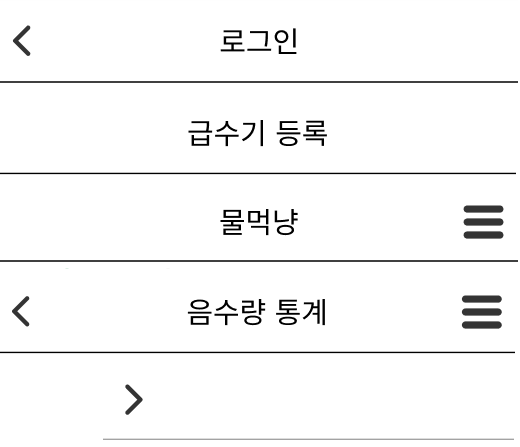
\includegraphics[width=0.3\textwidth]{img/Component/1.png}
    \item The title of the current screen appears in the center, and depending on what the current screen is, go back icon and menu icon are visible.
    \item It's also used in Drawer Navigation, where it turns into a close icon rather than a backward one. \\
\end{itemize}

\subsubsection{InputContainer}
\begin{itemize}
    \item[] 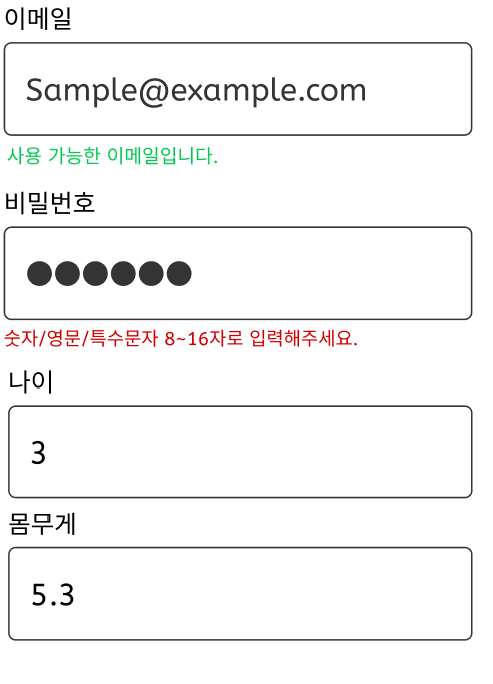
\includegraphics[width=0.27\textwidth]{img/Component/2.png}
    \item Used on the information input screen.
    \item The title on the top of the screen represents what that input screen is for and if input requirement is not satisfied, msg will deliver information on how to satisfy those input requirements.
    \item Input values such as password and password verification are made invisible.
    \item On each screen, it passes the required validation function to properly proceed with the validation. If the validation fails, the form submit button is not activated. \\
\end{itemize}

\newpage

\subsubsection{Button}
\begin{itemize}
    \item[] 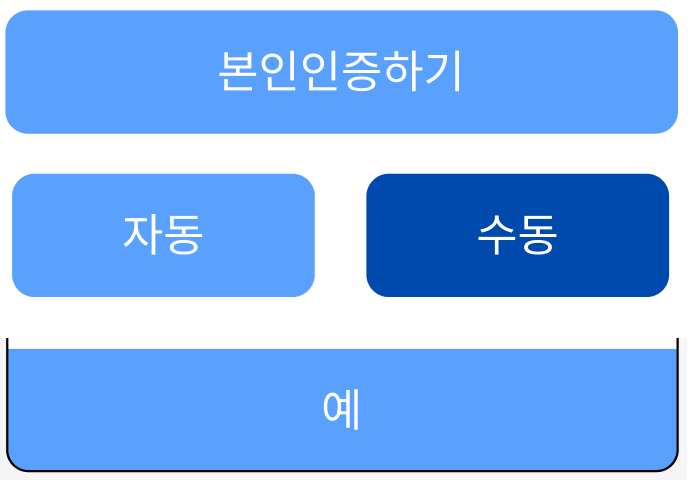
\includegraphics[width=0.25\textwidth]{img/Component/3.png}
    \item Title appear and indicate which button this is inside the button.
    \item If the button is inactivated, the color changes to navy.
    \item For optional buttons, reduce the size in half.
    \item When it is triggered by Alert Component, it replaces the border raidus to 0.
    \item Pass the handler function that needs to be executed on button click as a property.\\
\end{itemize}

\subsubsection{Alert}
\begin{itemize}
    \item[] 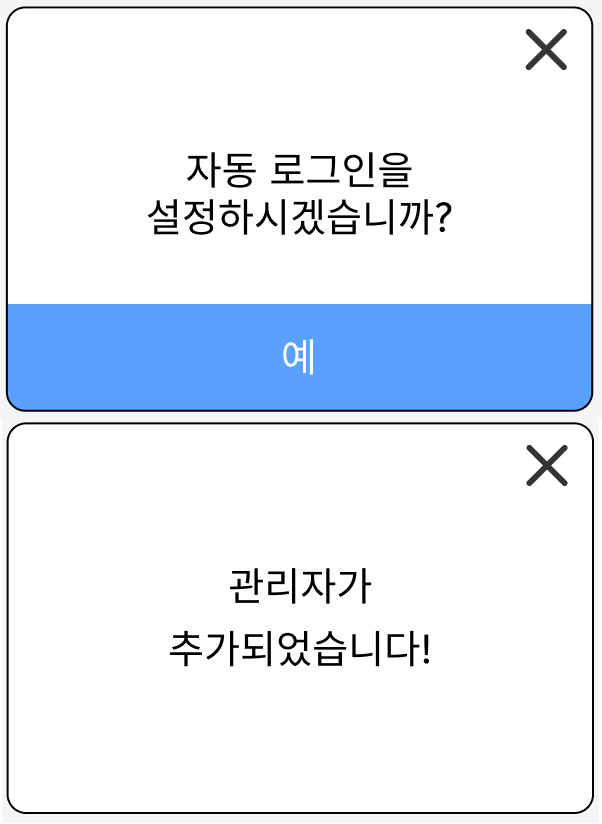
\includegraphics[width=0.2\textwidth]{img/Component/4.png}
    \item Once the data is registered or modified in the database after submitting the form, the database notifies you that the processing is complete.
    \item Before setting up auto login, it appears in the form with the button.
    \item When a button is pressed or when the close icon is clicked, if there's a need to navigate to another screen, we pass the name of the route to navigate to in the goRoute property. \\
\end{itemize}

\subsubsection{CatProfileList}
\begin{itemize}
    \item[] 
\includegraphics[width=0.3\textwidth]{img/Component/5.png}
    \item When you select a cat to display drink amount information on the Main Screen and Hydration Statistics Screen or when you select a cat to modify or delete information, CatProfileList appears.
    \item When the number of cats increases that the screen overflows, scroll feature is available.
    \item When a cat is selected, the catId value of that cat is stored in the global variable currentSelectedCat. \\
\end{itemize}

\subsection{Components Structure and Flow of each Screens}
The API that requires a detailed description of the API's call and processing process is described in detail in Section E.\\

\subsubsection{Start}
\begin{itemize}
    \item[] 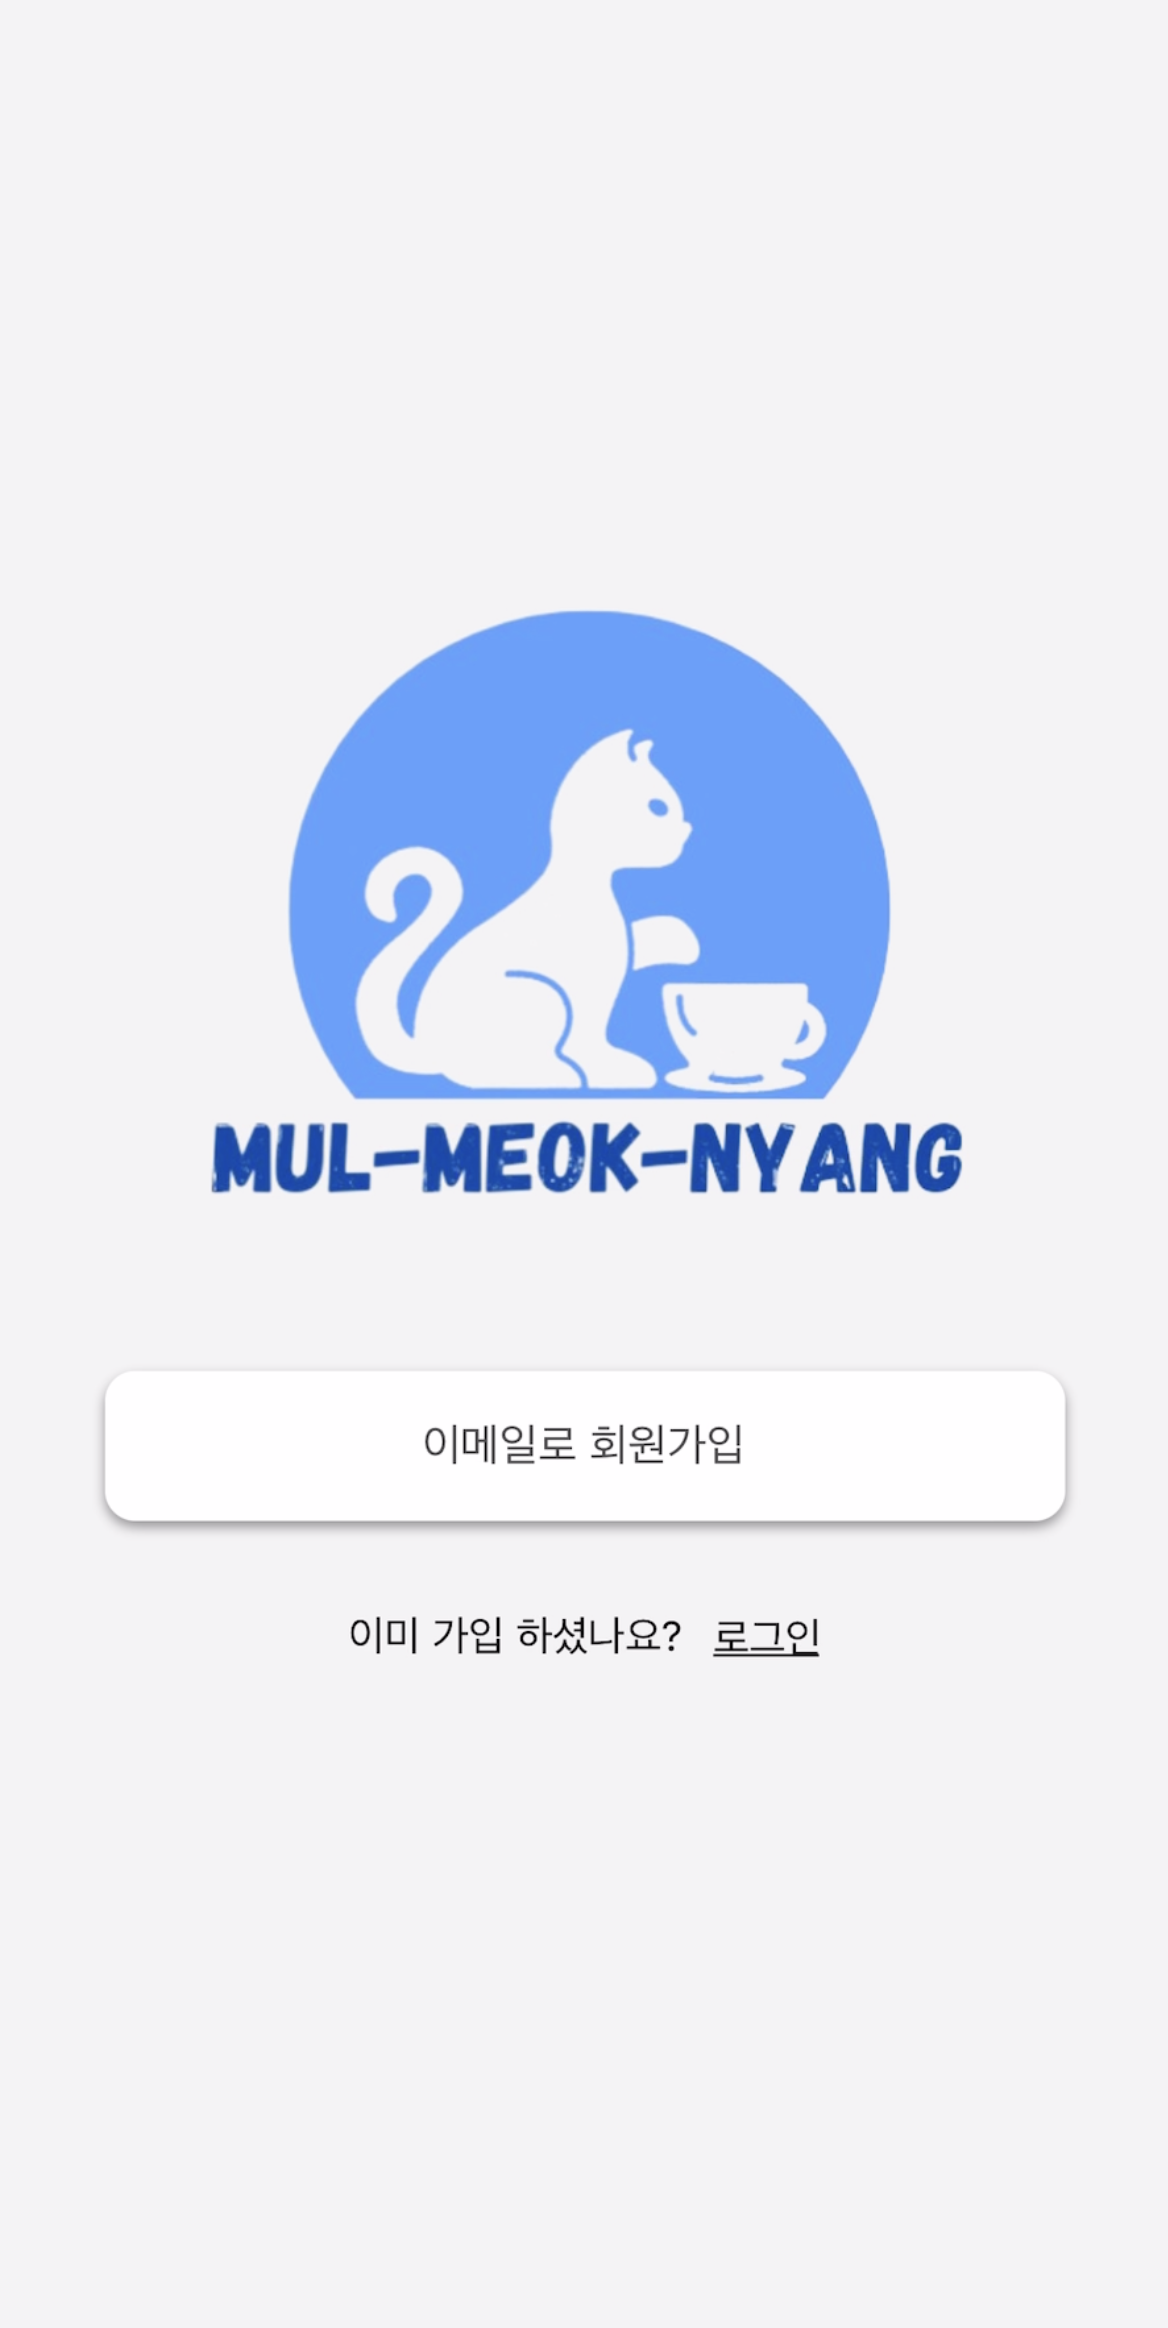
\includegraphics[width=0.27\textwidth]{img/Screen/1_Start.png}
    \item Components Structure of Screen
    \begin{itemize}
        \item Image Component
        \item SignUpButton Component
        \item Text Component
        \item UnderlineTextButton Component
    \end{itemize}
    \item Flow of Screen
    \begin{itemize}
        \item When the app starts, it makes sure that there is a Session ID Token in the React Native App Session storage.
        \item If token exists, it calls the AutoLogin API because user has auto-login enabled.
        \item When the button ‘SignUp by Email’ is pressed, it moves to the BasicForm Screen.
        \item When the button ‘\underline{Login}’ is pressed, it moves to the Login Screen. 
        \\
    \end{itemize}
\end{itemize}
\newpage

\subsubsection{LocalSignUp}
\begin{itemize}
    \item[] 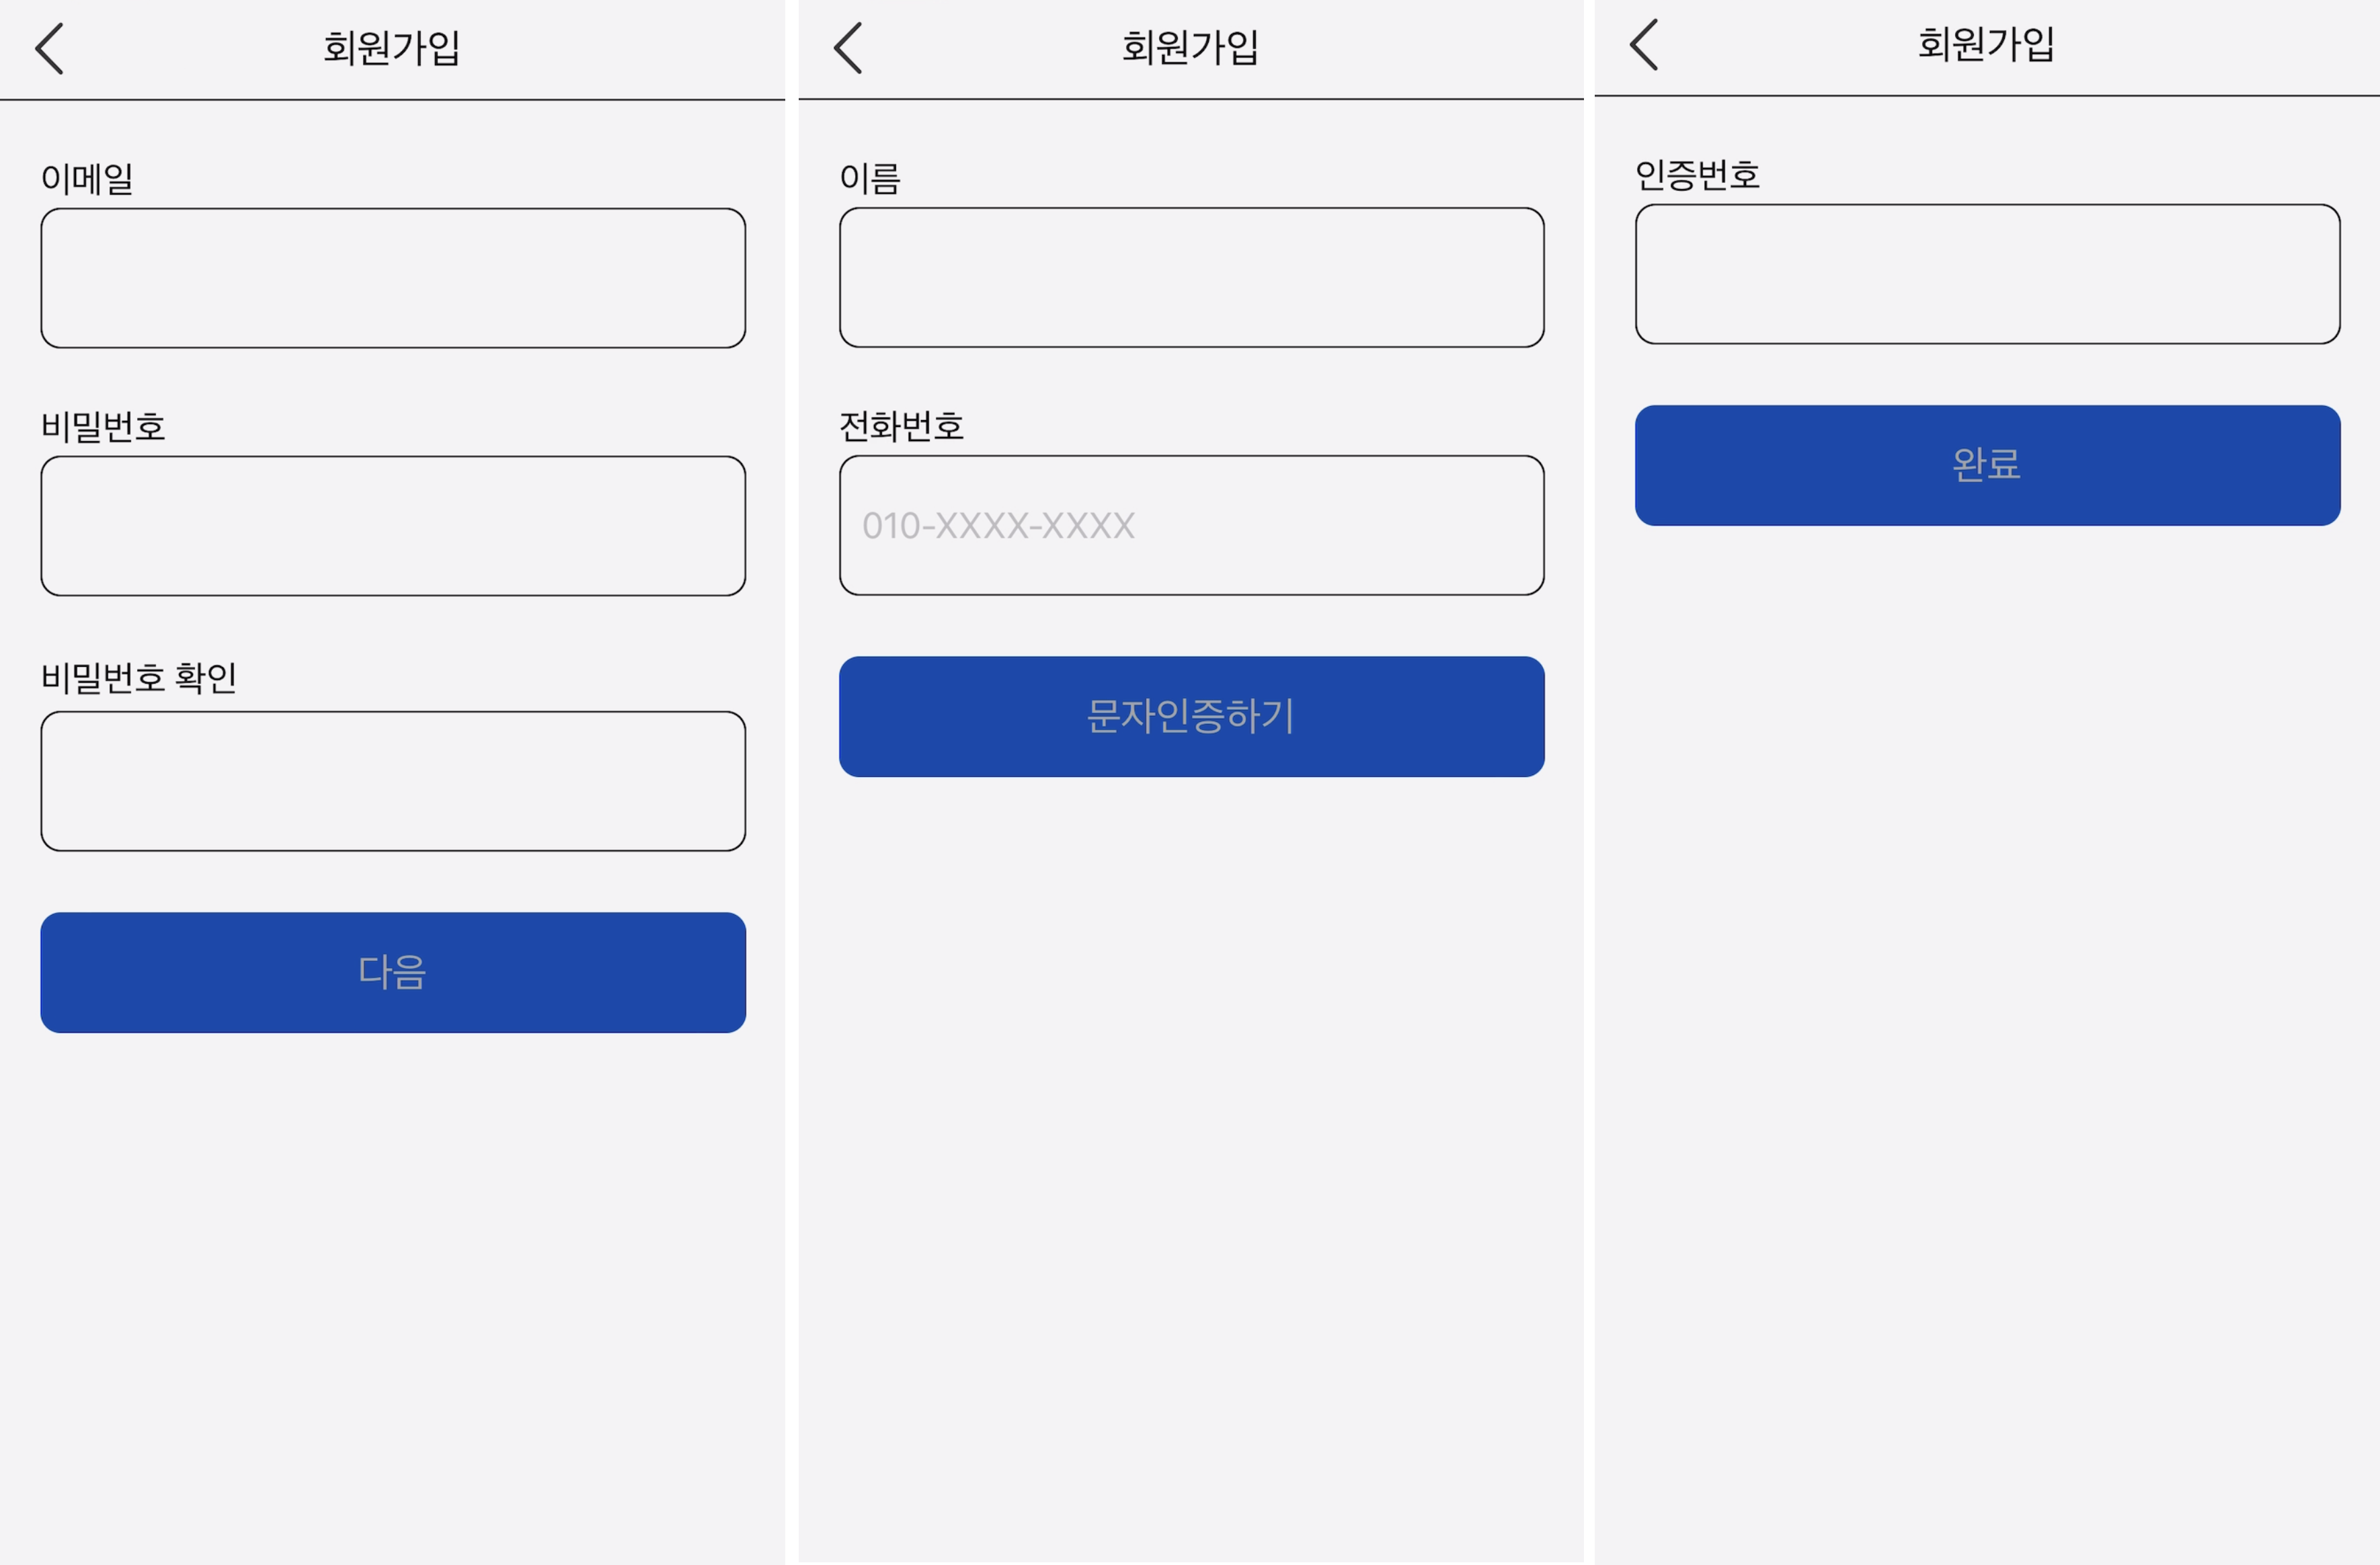
\includegraphics[width=0.45\textwidth]{img/Screen/2_SignUp.png}
    \item The BasicForm, RequestMessageAuth, and CheckMessageAuthCode screens in order.
    \item Components Structure of Screens
    \begin{itemize}
        \item TopBar Component
        \item InputContainer Component
        \begin{itemize}
            \item On the BasicForm Screen, checkEmailAvailable, checkPw, checkConrefmPw validation is performed, and the results are displayed below the input box.
            \item On the RequestMessageAuth Screen, checkEmpty, checkPhoneNum validation is performed, and the result of checkPhoneNum is only displayed below the input box.
            \item On the CheckMessageAuthCode Screen, checkEmpty validations is only performed.
        \end{itemize}
        \item Button Component
    \end{itemize}
    \item Flow of Screen
    \begin{itemize}
        \item Press the Go Back button to return to the previous Screen.
        \item On the BasicForm screen, when the email is entered in the correct format, the checkEmailAvailable API is called.
        \item If validation for email, password, and password confirmation passes, the 'Next' button becomes active, allowing navigation to the Request Message Auth screen.
        \item On the RequestMessageAuth screen, if validation for name and phone number passes, the 'Authenticate via Message' button becomes active. Pressing this button triggers the messageAuth API and moves to the CheckMessageAuthCode screen.
        \item Upon entering the authentication code, the 'Complete' button becomes active, triggering the checkMessageAuthCode API. If the authentication code doesn't match, an alert saying 'The authentication code doesn't match' appears.
        \item If the authentication code matches, the LocalSignUp API is called, completing the sign-up process and moving to the Login screen.
        \\
    \end{itemize}
\end{itemize}
\newpage

\subsubsection{Login}
\begin{itemize}
    \item[] 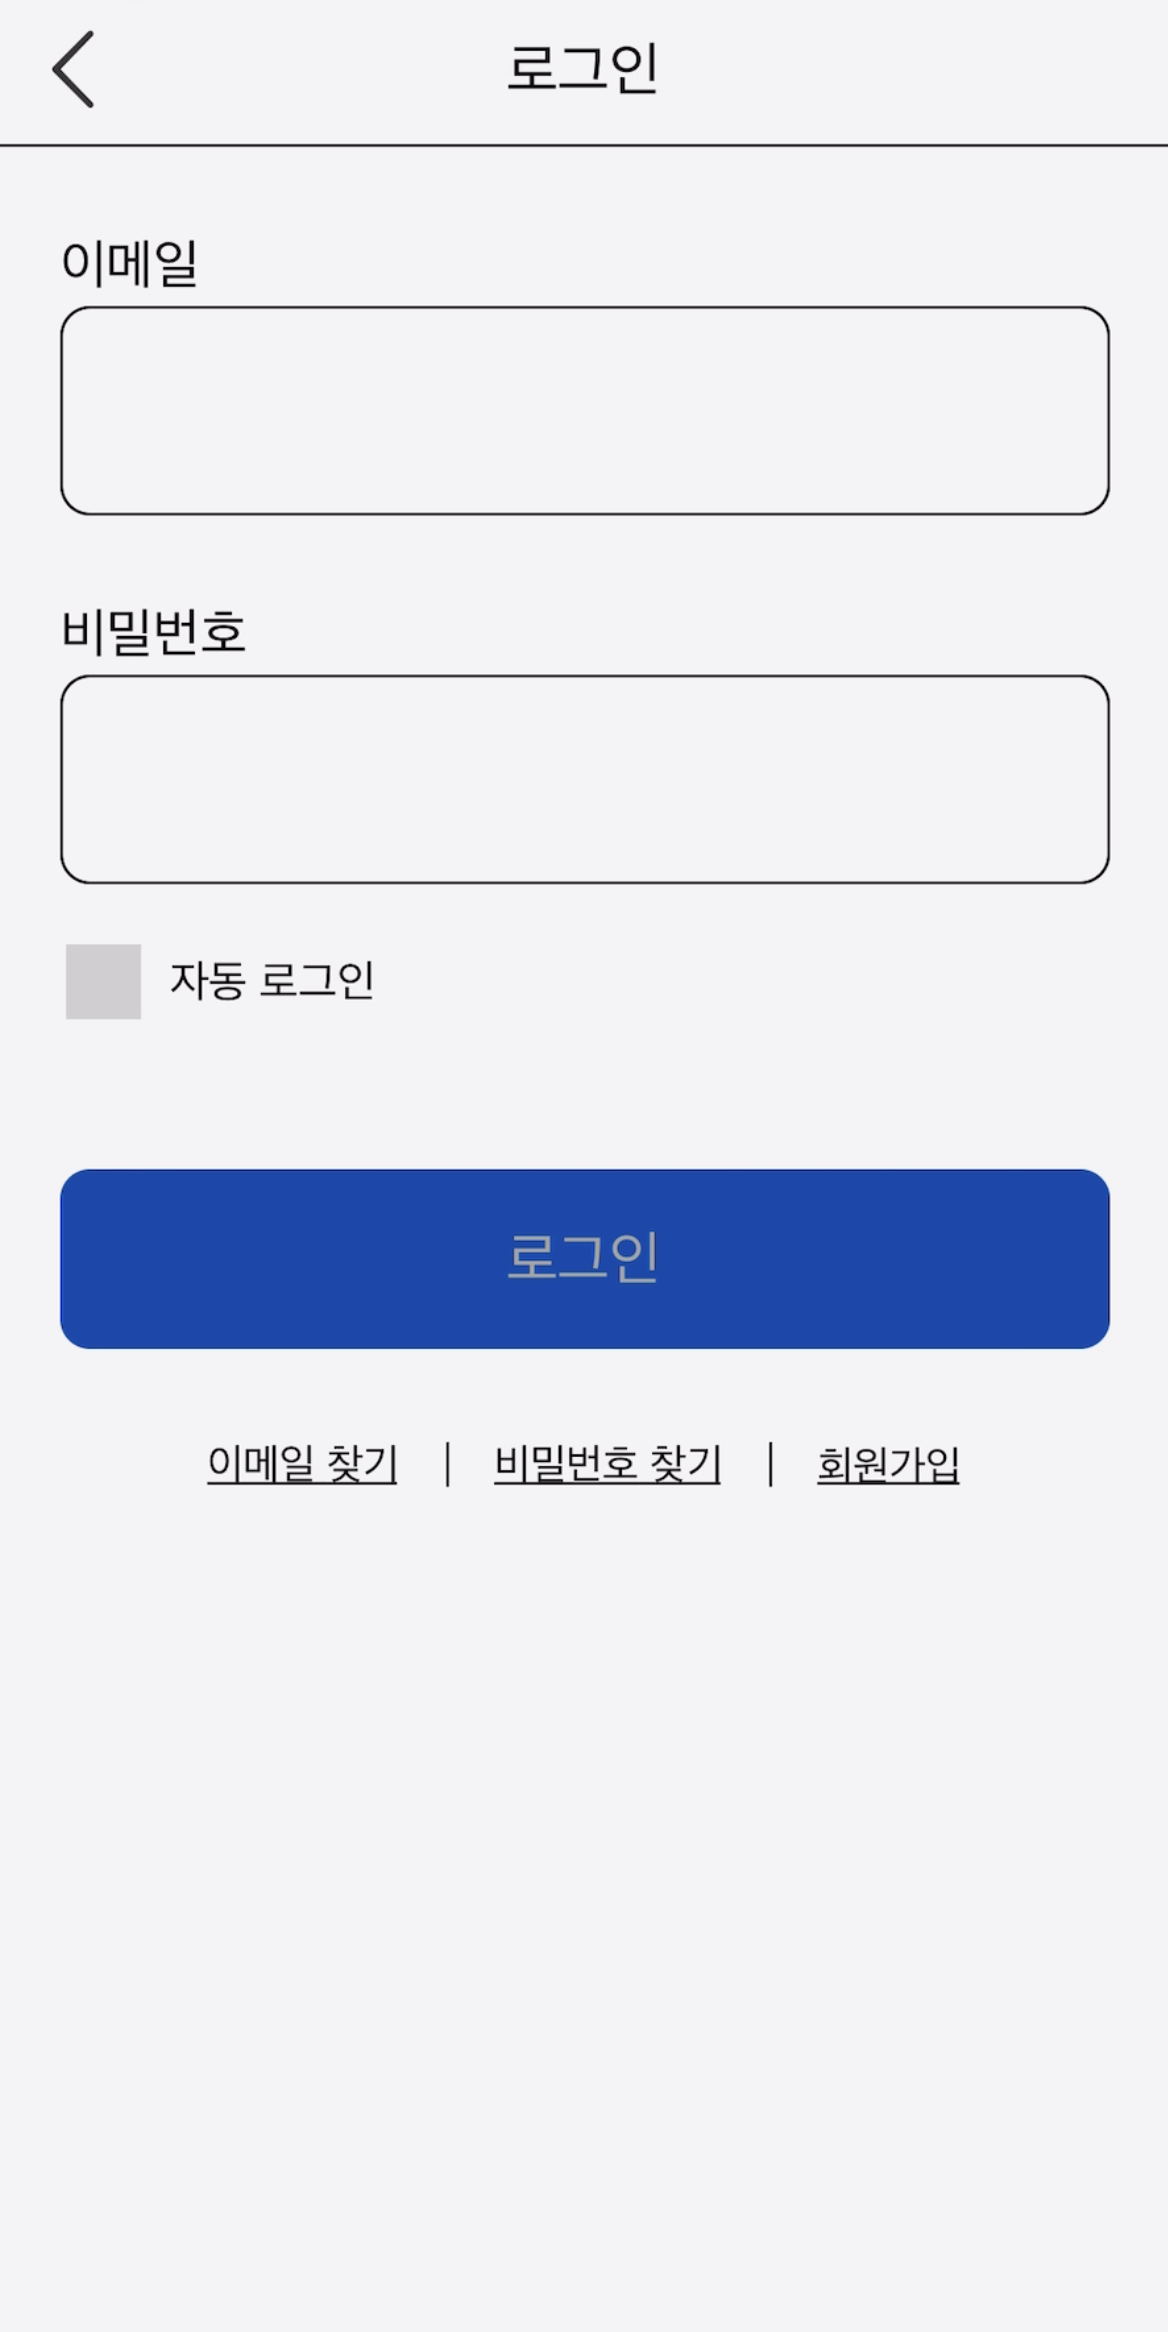
\includegraphics[width=0.27\textwidth]{img/Screen/3_Login.png}
    \item Components Structure of Screen
    \begin{itemize}
        \item TopBar Component
        \item InputContainer Component
        \begin{itemize}
            \item On the Login screen, only checkEmpty validation is performed.
        \end{itemize}
        \item AutoLoginCheckbox Component
        \item Button Component
        \item UnderlineTextButton Component
    \end{itemize}
    \item Flow of Screen
    \begin{itemize}
        \item Press the Go Back button to return to the previous Screen.
        \item Enter your email and password, select whether to log-in automatically, and press the 'Log in' button to call the Login API.
        \item When the button ‘\underline{Find Email}’ is pressed, moves to the FindEmail Screen.
        \item When the button ‘\underline{Find Pw}’ is pressed, moves to the FindPw Screen.
        \item When the button ‘\underline{Sign Up}’ is pressed, moves to the LocalSignUp Screen.
        \\
    \end{itemize}
\end{itemize}
\newpage

\subsubsection{FindEmail}
\begin{itemize}
    \item[] 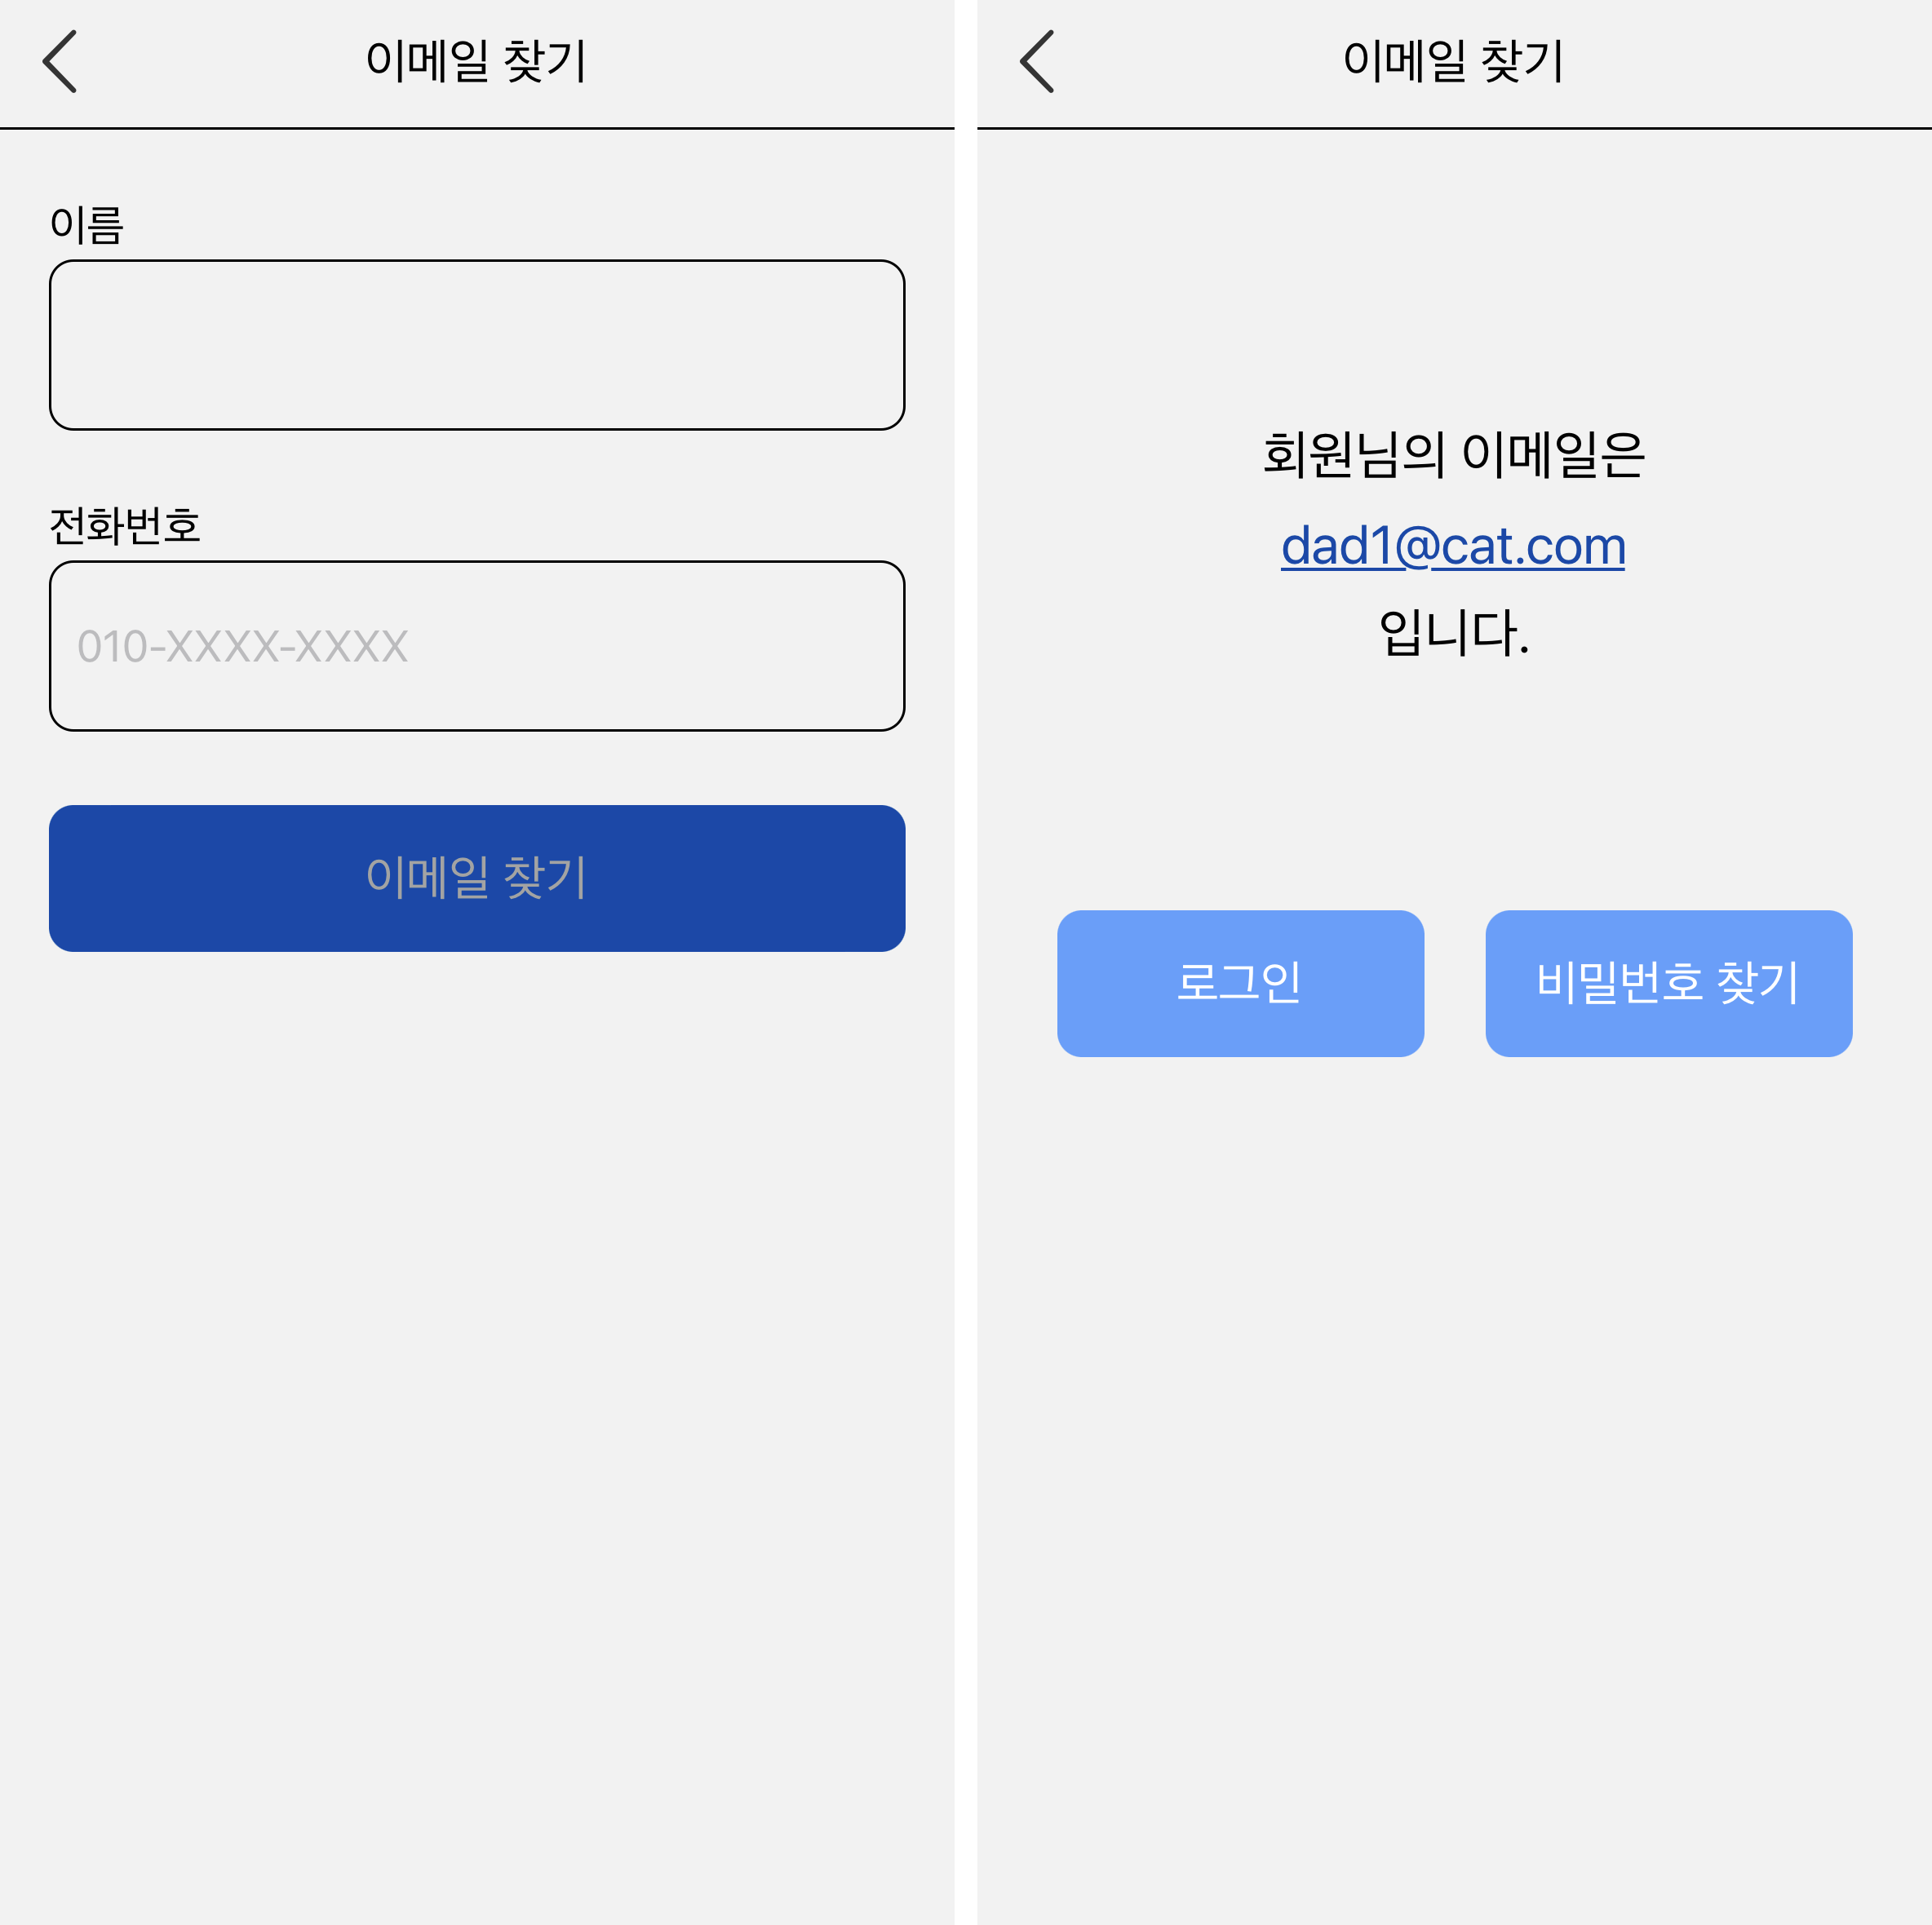
\includegraphics[width=0.45\textwidth]{img/Screen/4_FindEmail.png}
    \item The FindEmail and FindEmailResult screens in order.
    \item Components Structure of Screens
    \begin{itemize}
        \item TopBar Component
        \item InputContainer Component
        \begin{itemize}
            \item On the FindEmail screen, checkEmpty, checkPhoneNum validation is performed, and the results of the inspection are not displayed below the input box.
        \end{itemize}
        \item Text Component
        \item Button Component
    \end{itemize}
    \item Flow of Screen
    \begin{itemize}
        \item Press the Go Back button to return to the previous Screen.
        \item Enter your name and phone number, and press the '이메일 찾기' button to call the FindEmail API.
        \item If there is a serched email, move to the FindEmailResult screen and display the respective email.
        \item When the button ‘{Login}’ is pressed, moves to the FindEmail Screen.
        \item When the button ‘{Find Pw}’ is pressed, moves to the FindEmail Screen.
        \\
    \end{itemize}
\end{itemize}
\newpage

\subsubsection{FindPw}
\begin{itemize}
    \item[] 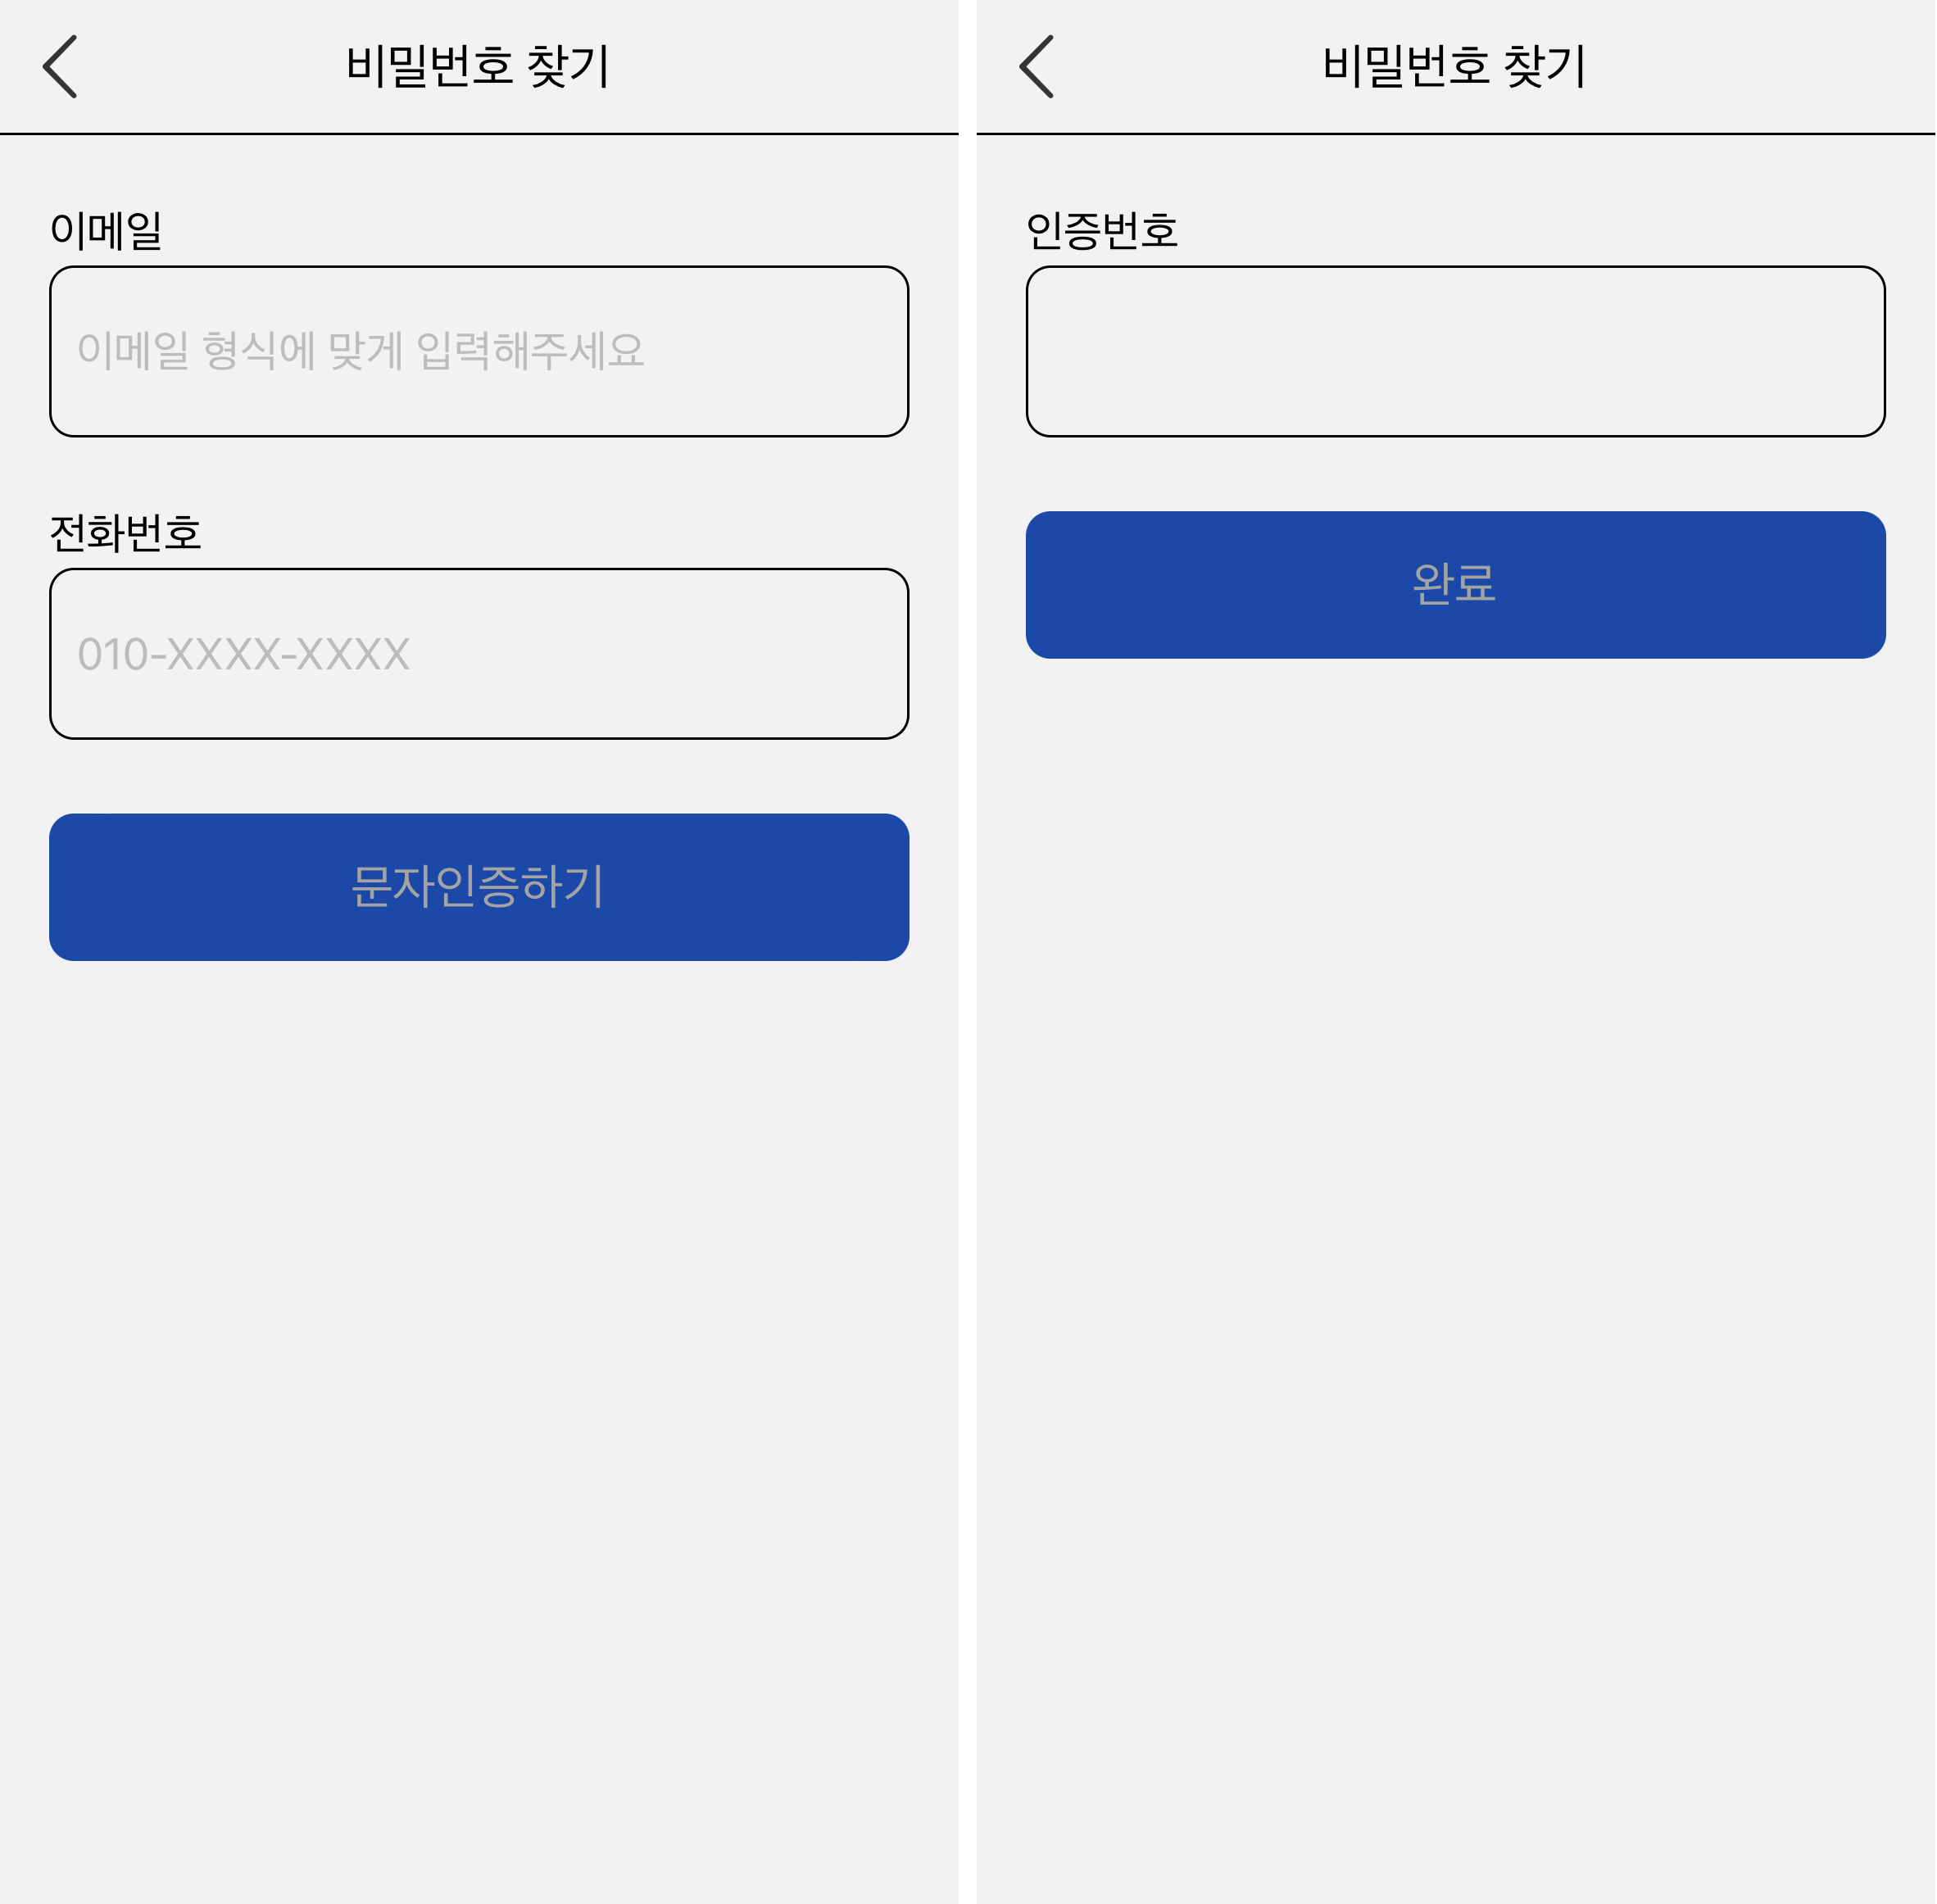
\includegraphics[width=0.45\textwidth]{img/Screen/5_FindPw.png}
    \item The FindPw and CheckMessageAuthCode screens in order.
    \item Components Structure of Screens
    \begin{itemize}
        \item TopBar Component
        \item InputContainer Component
        \begin{itemize}
            \item On the FindPw screen, a checkEmail validation is performed, and the results are displayed below the input box.
            \item On the CheckMessageAuthCode screen, a checkEmpty validation is only performed.
        \end{itemize}
        \item Button Component
    \end{itemize}
    \item Flow of Screen
    \begin{itemize}
        \item Press the Go Back button to return to the previous Screen.
        \item If both email and phone number validations pass, the 'Authenticate via Message' button becomes active. Upon clicking the button, it triggers the messageAuth API and moves to the Check Message Auth Code screen.
        \item Once the authentication code is entered, the 'Complete' button becomes active, triggering the checkMessageAuthCode API first. If the authentication code doesn't match, an alert saying 'The authentication code doesn't match' appears.
        \item If the authentication code matches, it calls the SendPw API.
        \\
    \end{itemize}
\end{itemize}
\newpage

\subsubsection{UserProfileRegistration}
\begin{itemize}
    \item[] 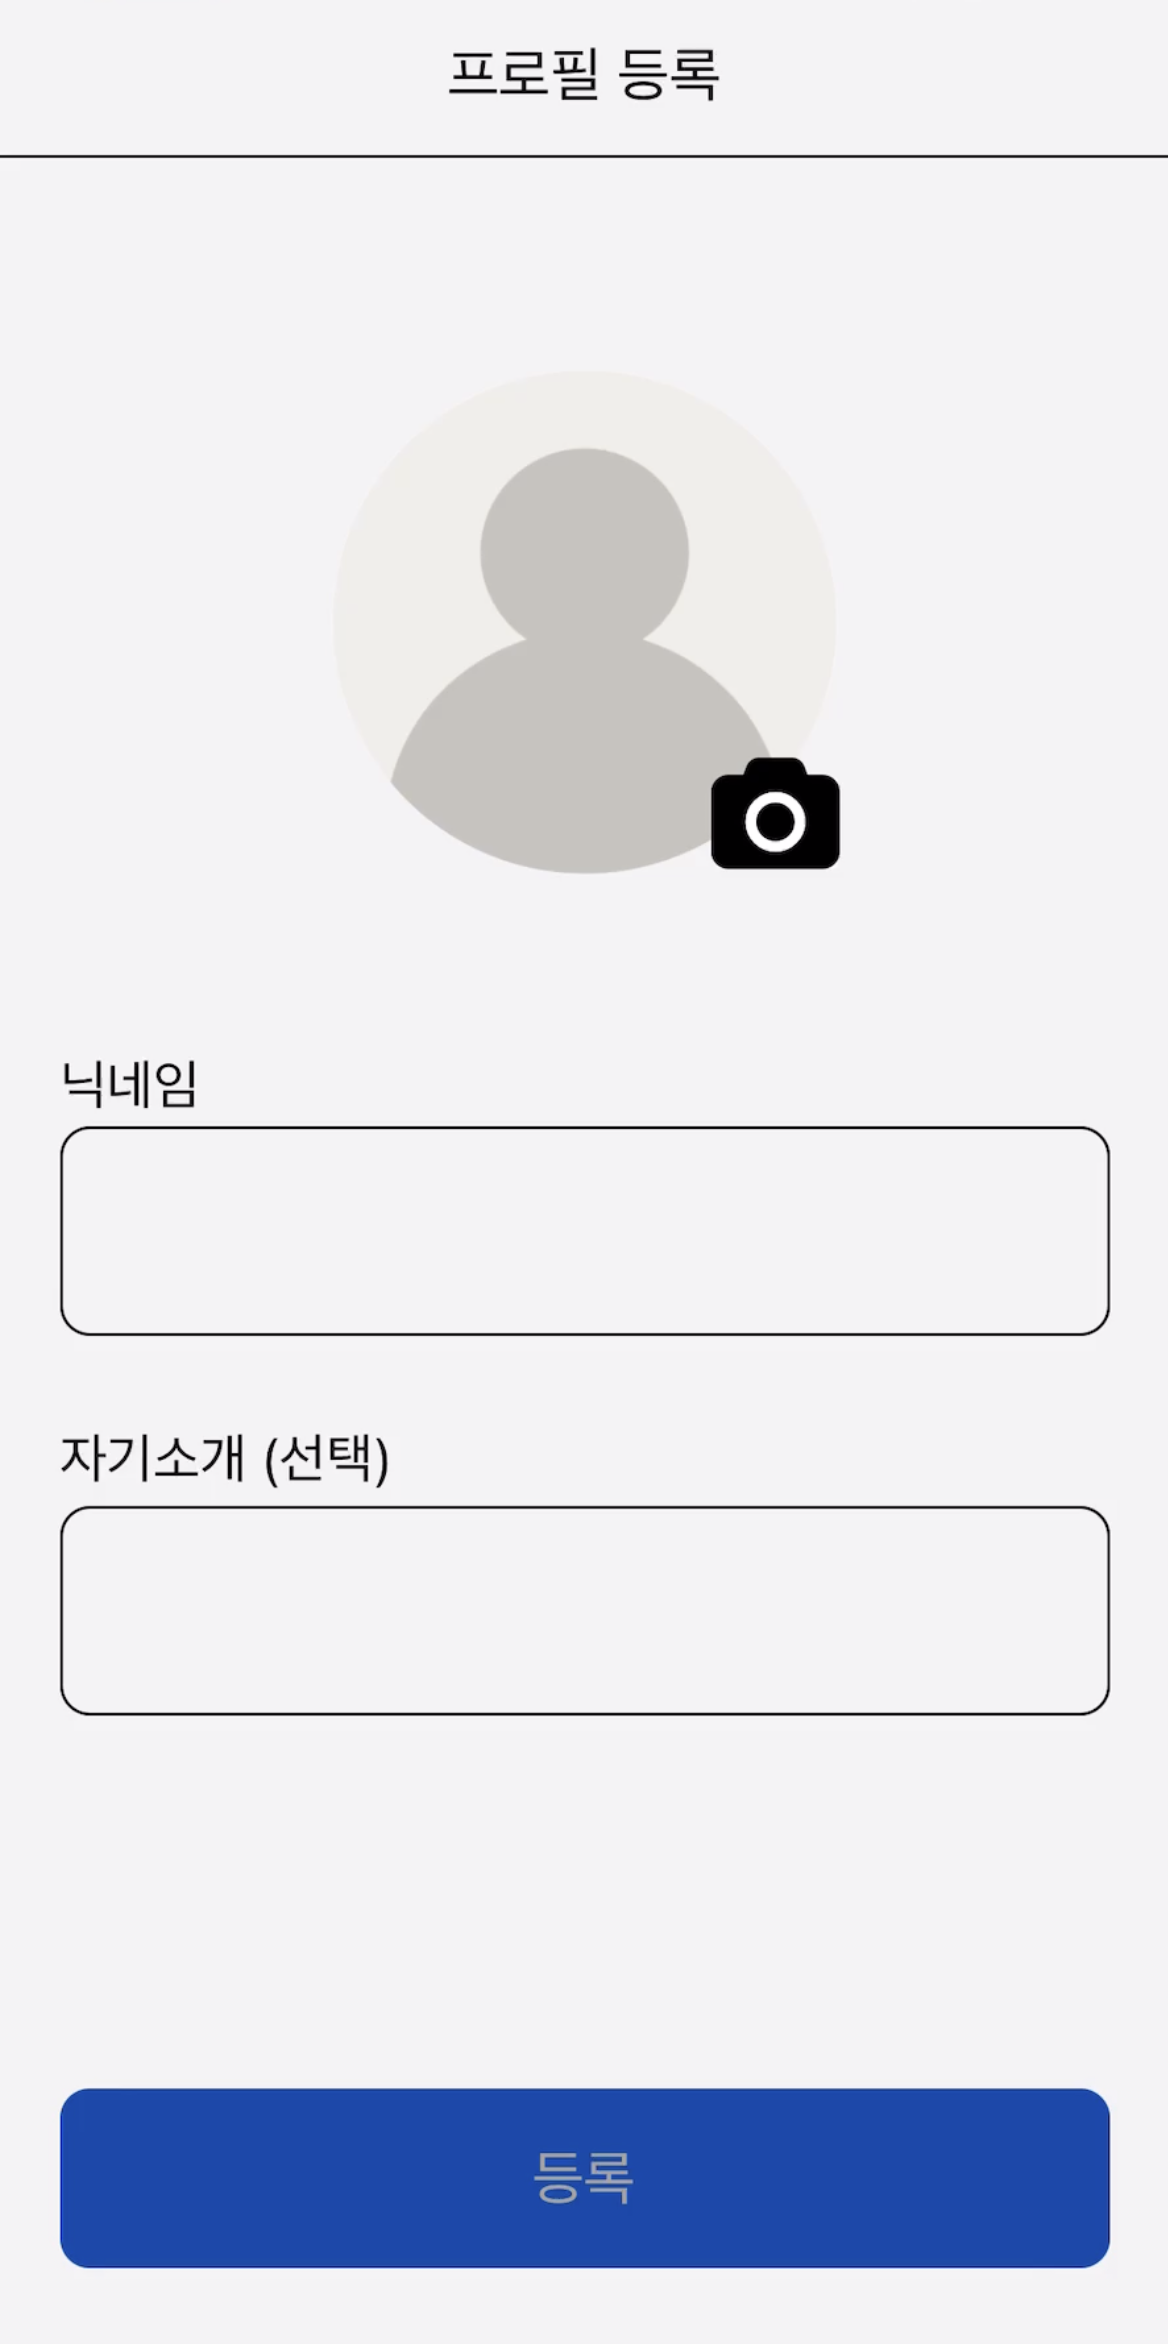
\includegraphics[width=0.27\textwidth]{img/Screen/6_UserProfile.png}
    \item Components Structure of Screen
    \begin{itemize}
        \item TopBar Component
        \item ImageInputContainer Component
        \begin{itemize}
            \item Uses react-native-image-picker package.
        \end{itemize}
        \item InputContainer Component
        \begin{itemize}
            \item On the UserProfileRegistration Screen, only the nickname performs a checkEmpty validation, and the result of the check is not displayed below the input box.
        \end{itemize}
        \item Button Component
    \end{itemize}
    \item Flow of Screen
    \begin{itemize}
        \item Press the camera button to select a profile photo from user's gallery.
        \item Enter the nickname, which is mandatory, and press the 'Completion' button to call the RegisterUserProfile API.
        \\
    \end{itemize}
\end{itemize}
\newpage

\subsubsection{PrepareSpace}
\begin{itemize}
    \item[] 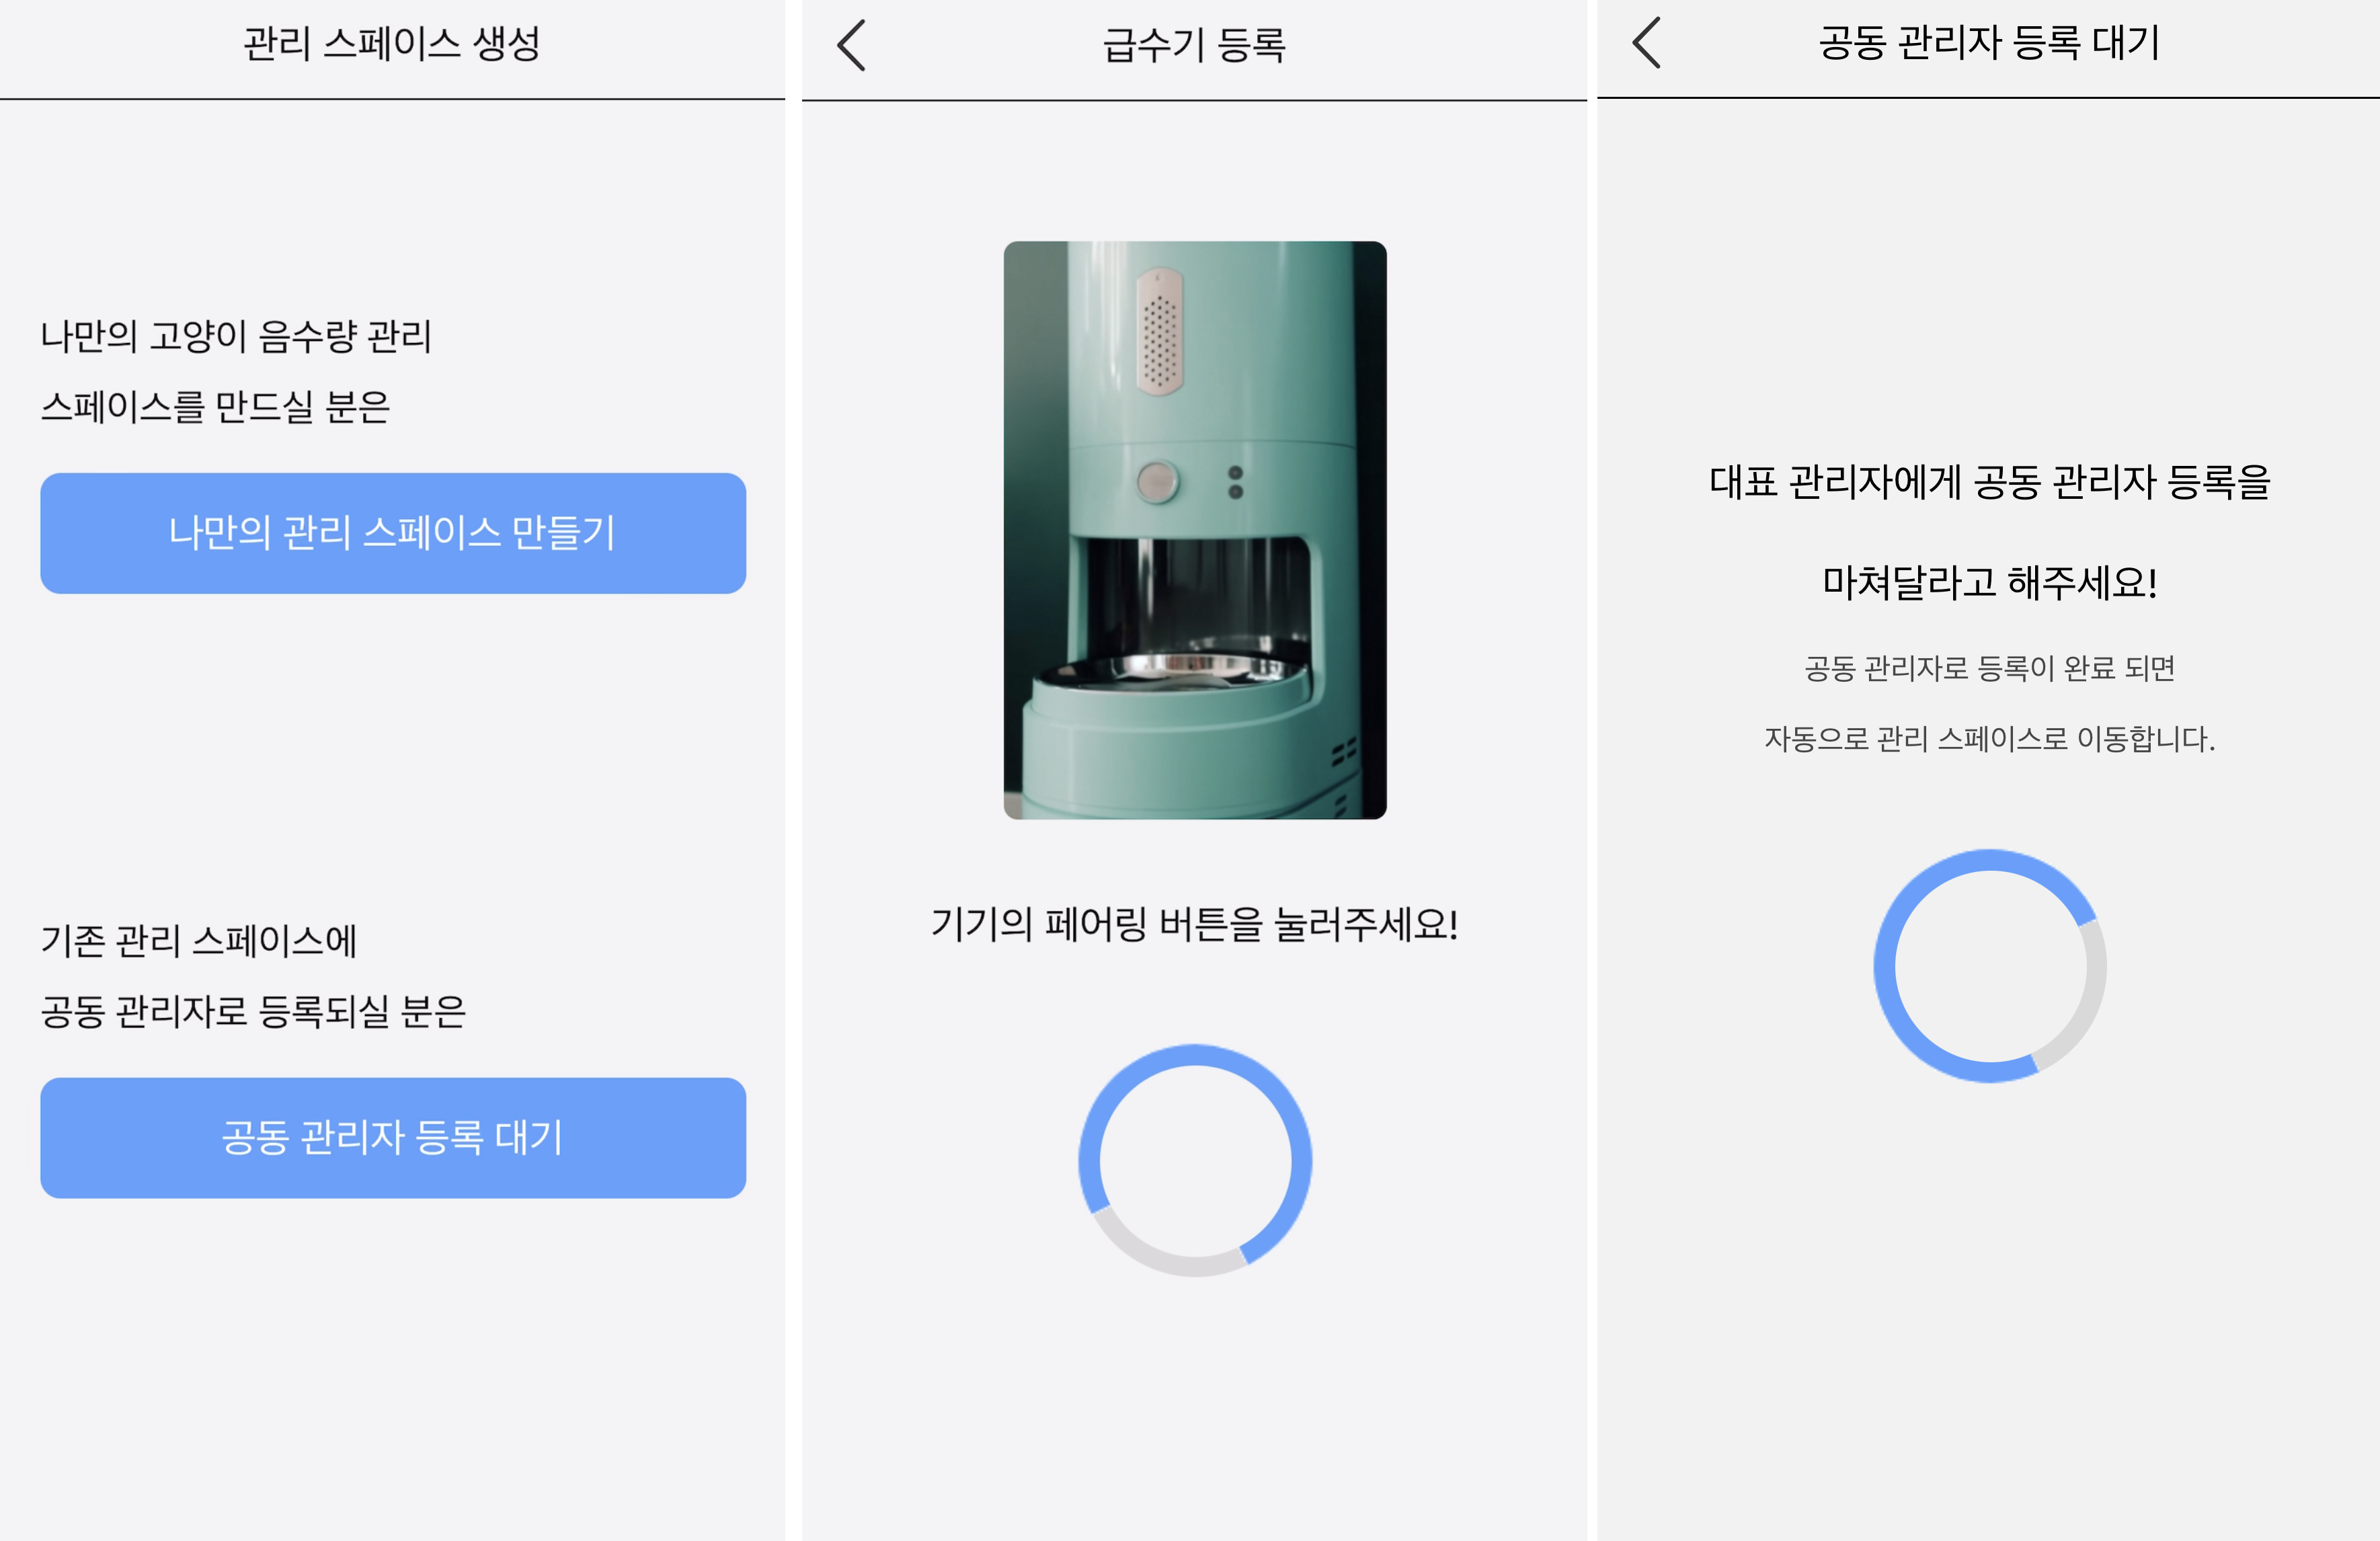
\includegraphics[width=0.45\textwidth]{img/Screen/7, 8.png}
    \item The HowToGoSpace, DeviceRegistration and PendingCoManagerAddition screens in order.
    \item HowToGoSpace
    \begin{itemize}
        \item Components Structure of Screen
        \begin{itemize}
            \item TopBar Component
            \item Text Component
            \item Button Component
        \end{itemize}
        \item Flow of Screen
        \begin{itemize}
            \item Press the 'Create my own management space' button to go to the DeviceRegistration Screen.
            \item Press the 'Pending on Co-Manager Addition' button to go to the PendingCoManagerAddition Screen.
            \\
        \end{itemize}
    \end{itemize}
    \item DeviceRegistration
    \begin{itemize}
        \item Components Structure of Screen
        \begin{itemize}
            \item TopBar Component
            \item Image Component
            \item Text Component
            \item Loading Component
            \item Button Component
            \item DeviceSelect Component
            \item[] 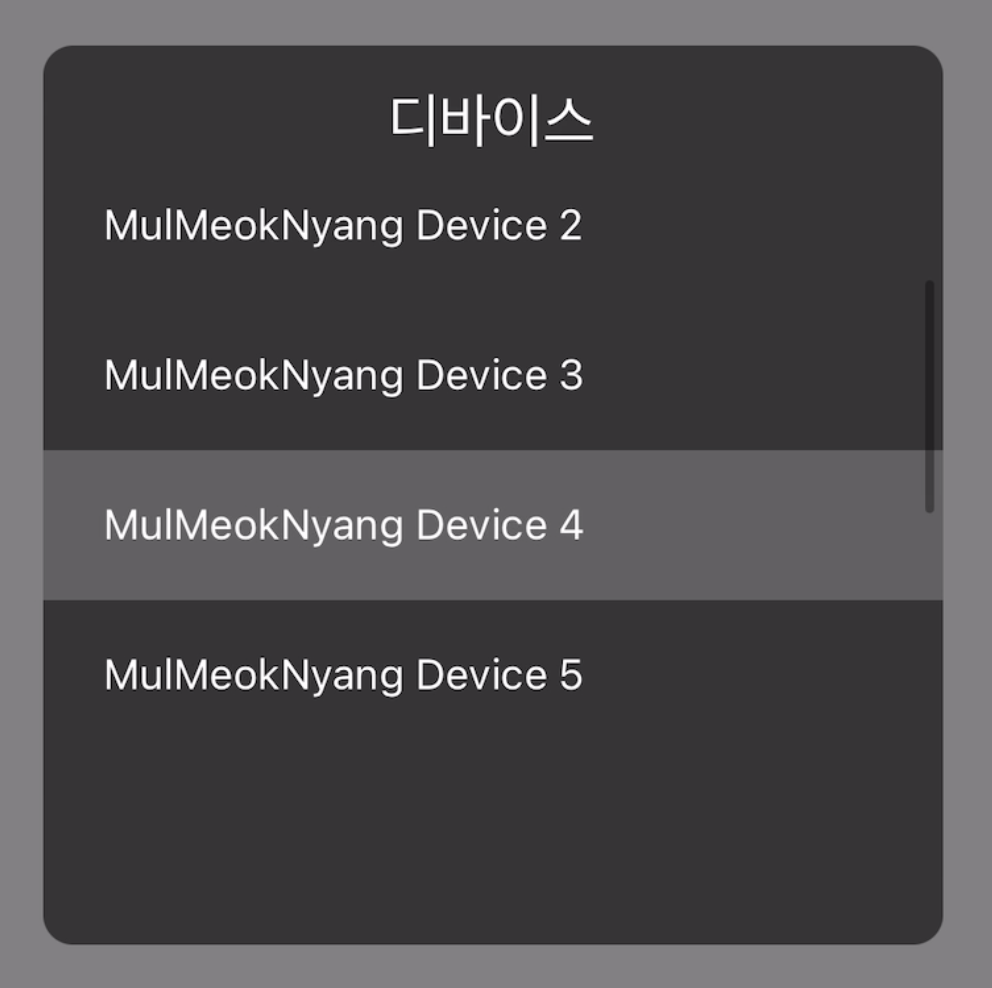
\includegraphics[width=0.2\textwidth]{img/Screen/8_Device2.png}
        \end{itemize}
        \item Instead of Using API
        \begin{itemize}
            \item Since the device cannot actually be registered, it shows an animation during loading for 3 seconds, assuming that the pairing button is being pressed.
            \item Then, the Device Select Component is displayed and when the user selects Device, the property value of the Loading Component is changed to false and shows the pairing completed animation. Then it goes to the CatProfileRegistration Screen.
            \\
        \end{itemize}
    \end{itemize}
    \item PendingCoManagerAddition
    \begin{itemize}
        \item Components Structure of Screen
        \begin{itemize}
            \item TopBar Component
            \item Text Component
            \item Loading Component
        \end{itemize}
        \item Flow of Screen
        \begin{itemize}
            \item Press the Back button to call the clearInterval function and return to the previous Screen.
            \item Use the setInterval function to call the GetManagementSpaceId API every 5 seconds until you are registered as a co-administrator.
            \\
        \end{itemize}
    \end{itemize}
\end{itemize}

\subsubsection{CatProfileRegistration}
\begin{itemize}
    \item[] 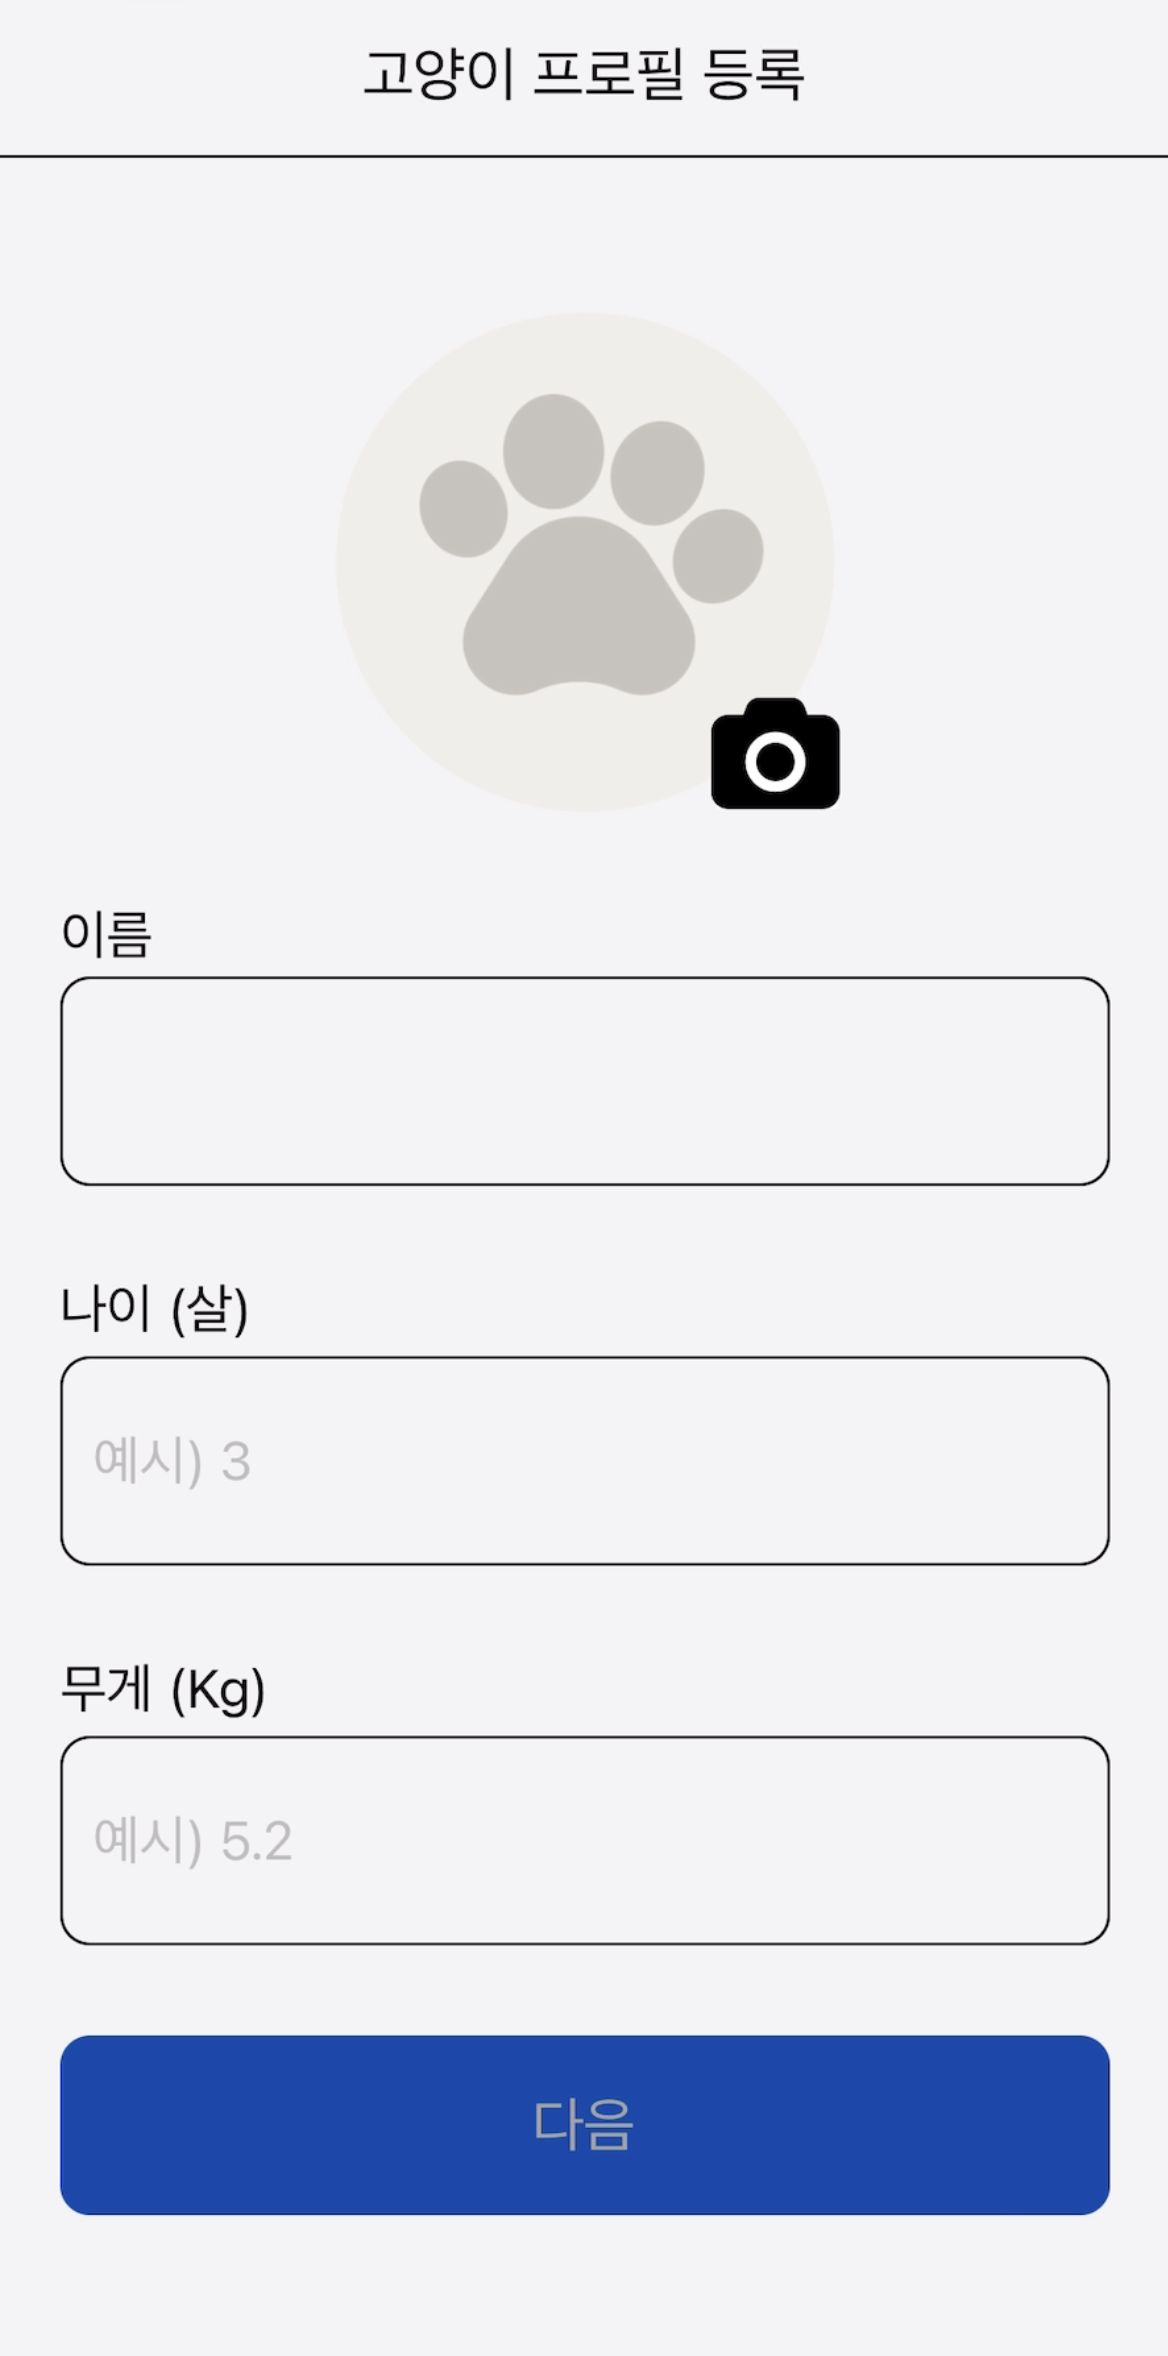
\includegraphics[width=0.27\textwidth]{img/Screen/10_CatProfile.png}
    \item Components Structure of Screen
    \begin{itemize}
        \item TopBar Component
        \item ImageInputContainer Component
        \item InputContainer Component
        \begin{itemize}
            \item On the CatProfileRegistration screen, a checkEmpty validation is only performed.
        \end{itemize}
        \item Button Component
    \end{itemize}
    \item Flow of Screen
    \begin{itemize}
        \item Press the camera button to select a profile photo from user's gallery.
        \item Enter a name, age, and weight, and press the Next button to save the catName, catAge, and catWeight global variables with the Context API and moves to CatPhotosRegistration Screen.
    \end{itemize}
\end{itemize}
\newpage

\subsubsection{CatPhotosforAISet}
\begin{itemize}
    \item[] 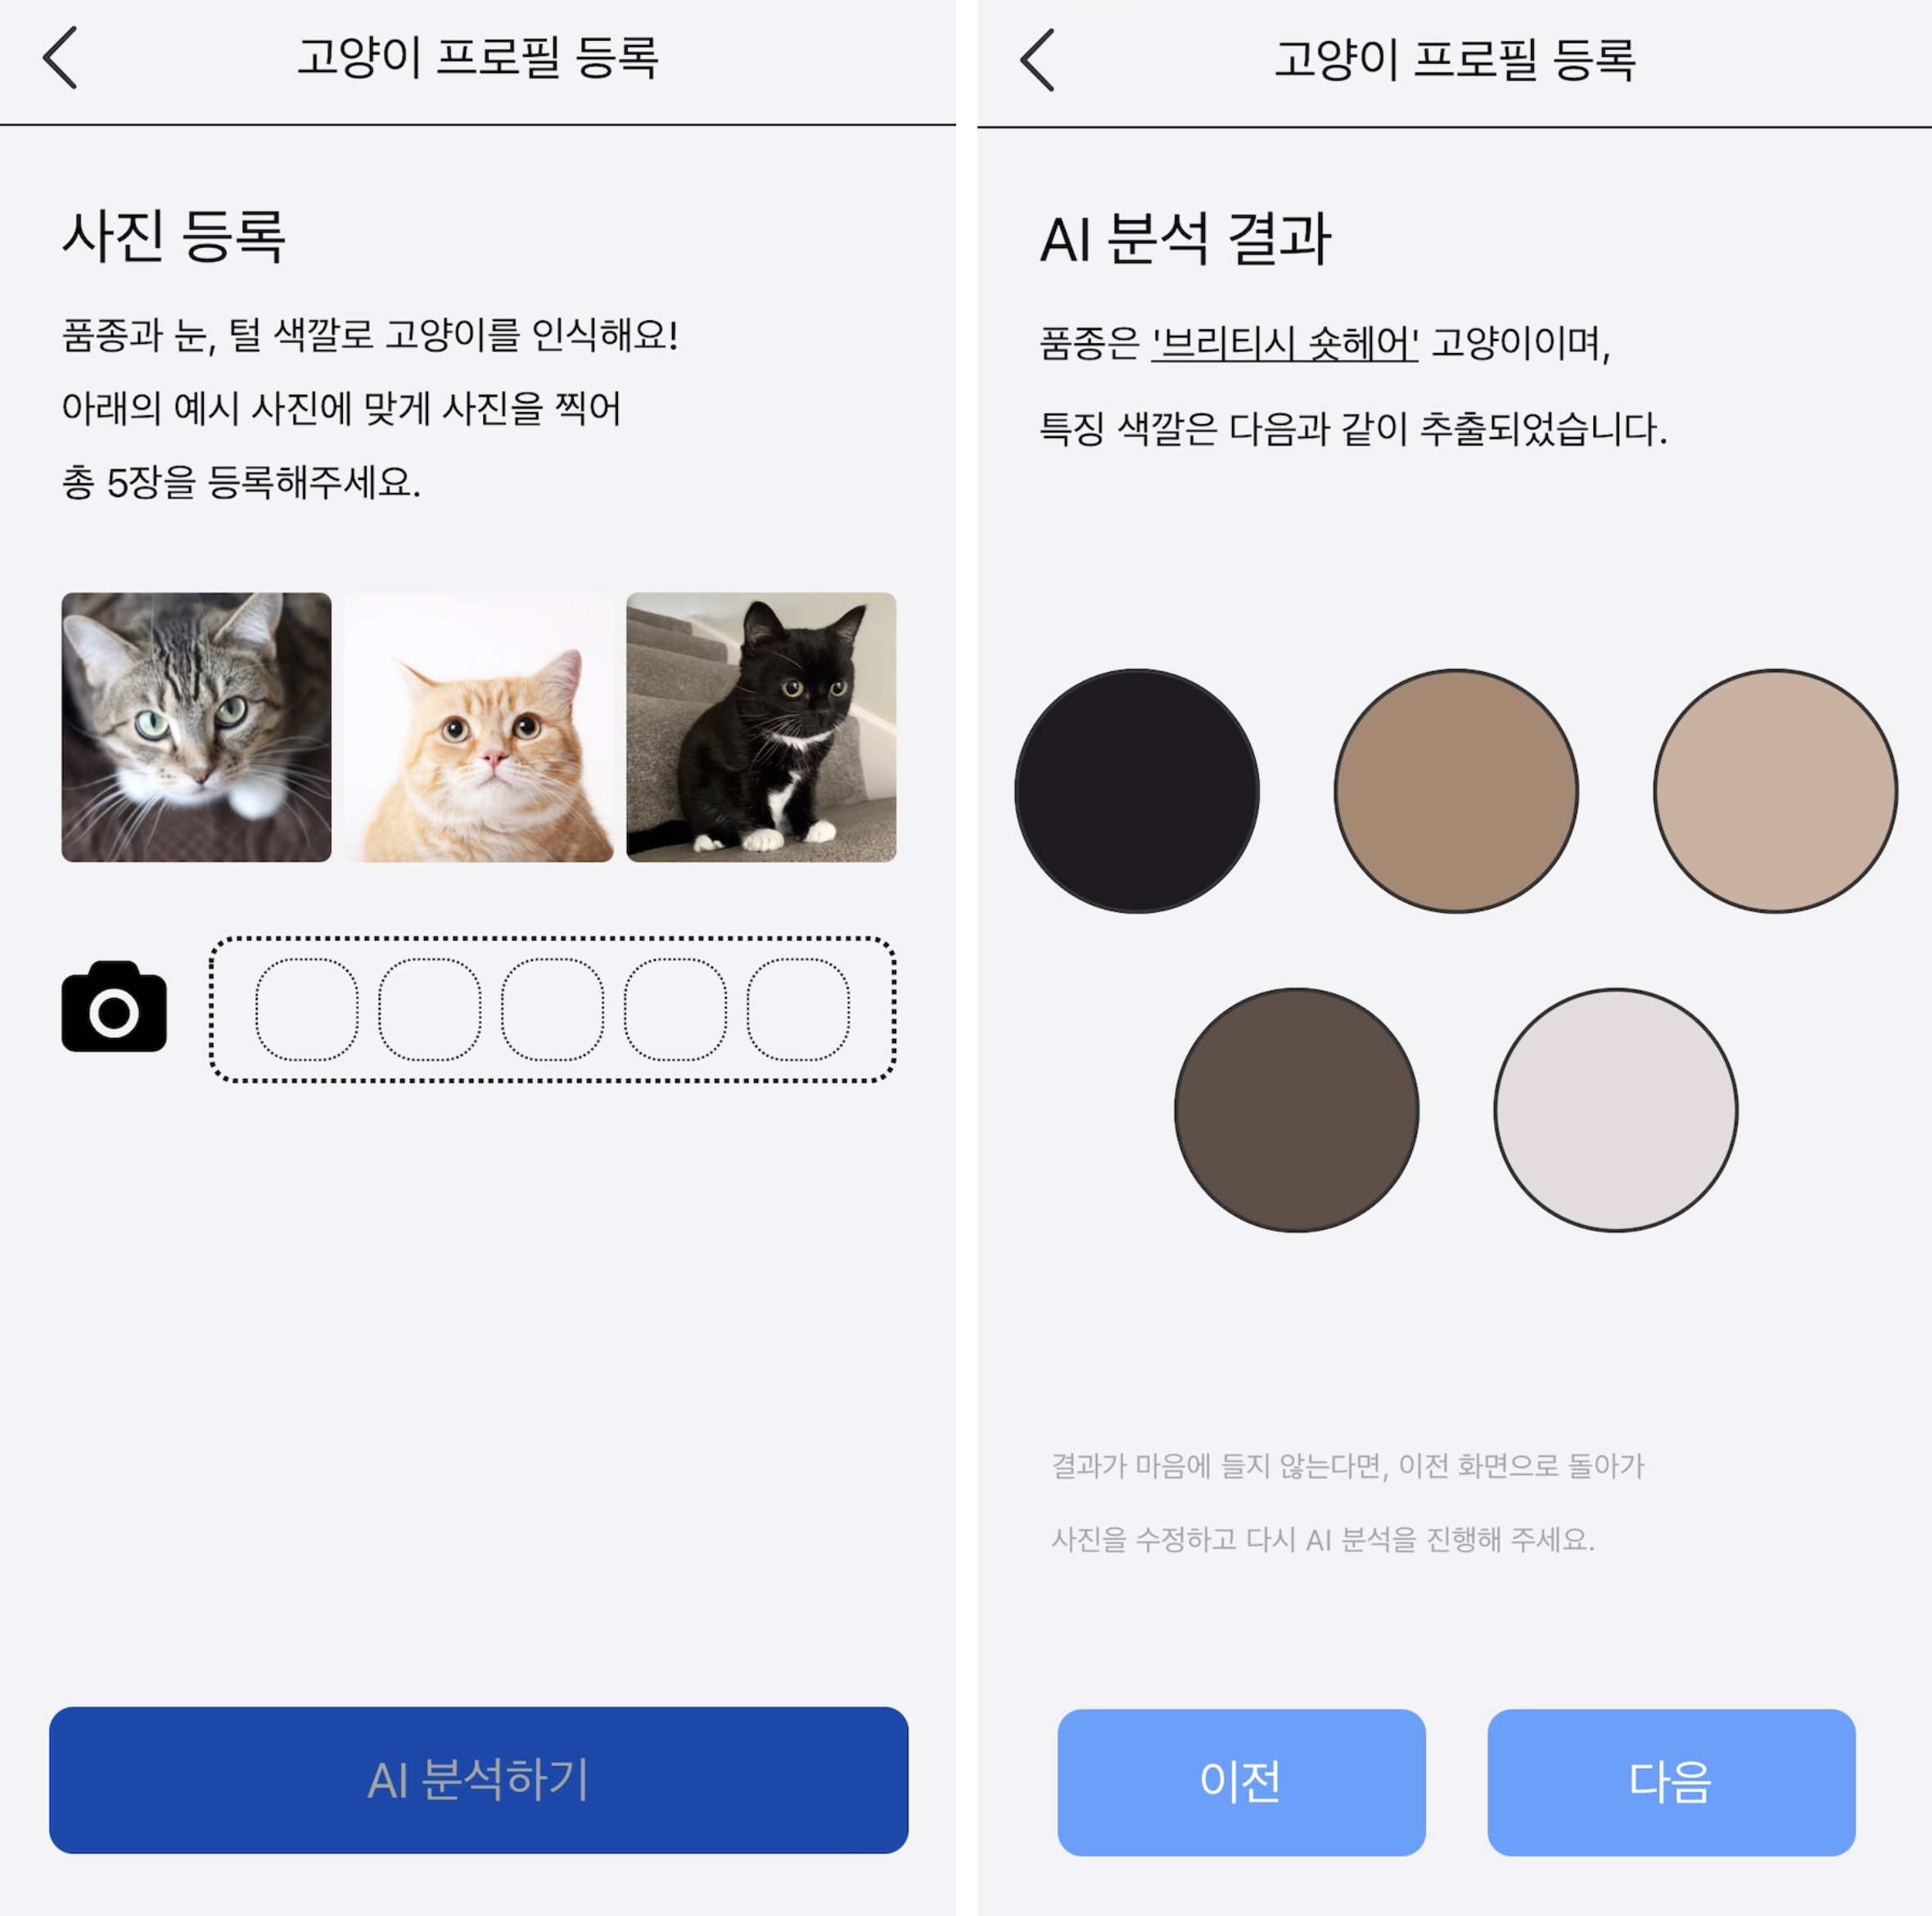
\includegraphics[width=0.45\textwidth]{img/Screen/11.png}
    \item The CatPhotosForAIRegistration and AIResult screens in order.
    \item CatPhotosForAIRegistration
    \begin{itemize}
        \item Components Structure of Screen
        \begin{itemize}
            \item TopBar Component
            \item Text Component
            \item Image Component
            \item Icon Component
            \item FlatList Component
            \item Button Component
            \begin{itemize}
                \item User must register 5 photos to activate the button.
            \end{itemize}
        \end{itemize}
        \item Flow of Screen
        \begin{itemize}
            \item Press the Go Back button to return to the previous Screen.
            \item Upon tapping the camera button and selecting photos from the gallery, a total of 5 photos are uploaded. Afterward, pressing the 'AI Analysis' button triggers the CallAI API.
            \item Upon receiving the AI analysis results, it moves to the AI Result screen\\
        \end{itemize}
    \end{itemize}
    \item AIResult
    \begin{itemize}
        \item Components Structure of Screen
        \begin{itemize}
            \item TopBar Component
            \item Text Component
            \item Circle Component
            \item Button Component
        \end{itemize}
        \item Flow of Screen
        \begin{itemize}
            \item Pressing the 'Previous' button will navigate back to the previous screen, allowing for a re-analysis via AI.
            \item Pressing the 'Next' button saves the global variables catBreed and catColor via the Context API, then moves to the CatFeedStuffRegistration screen.\\
        \end{itemize}
    \end{itemize}
\end{itemize}

\subsubsection{CatFeedStuffRegistration}
\begin{itemize}
    \item[] 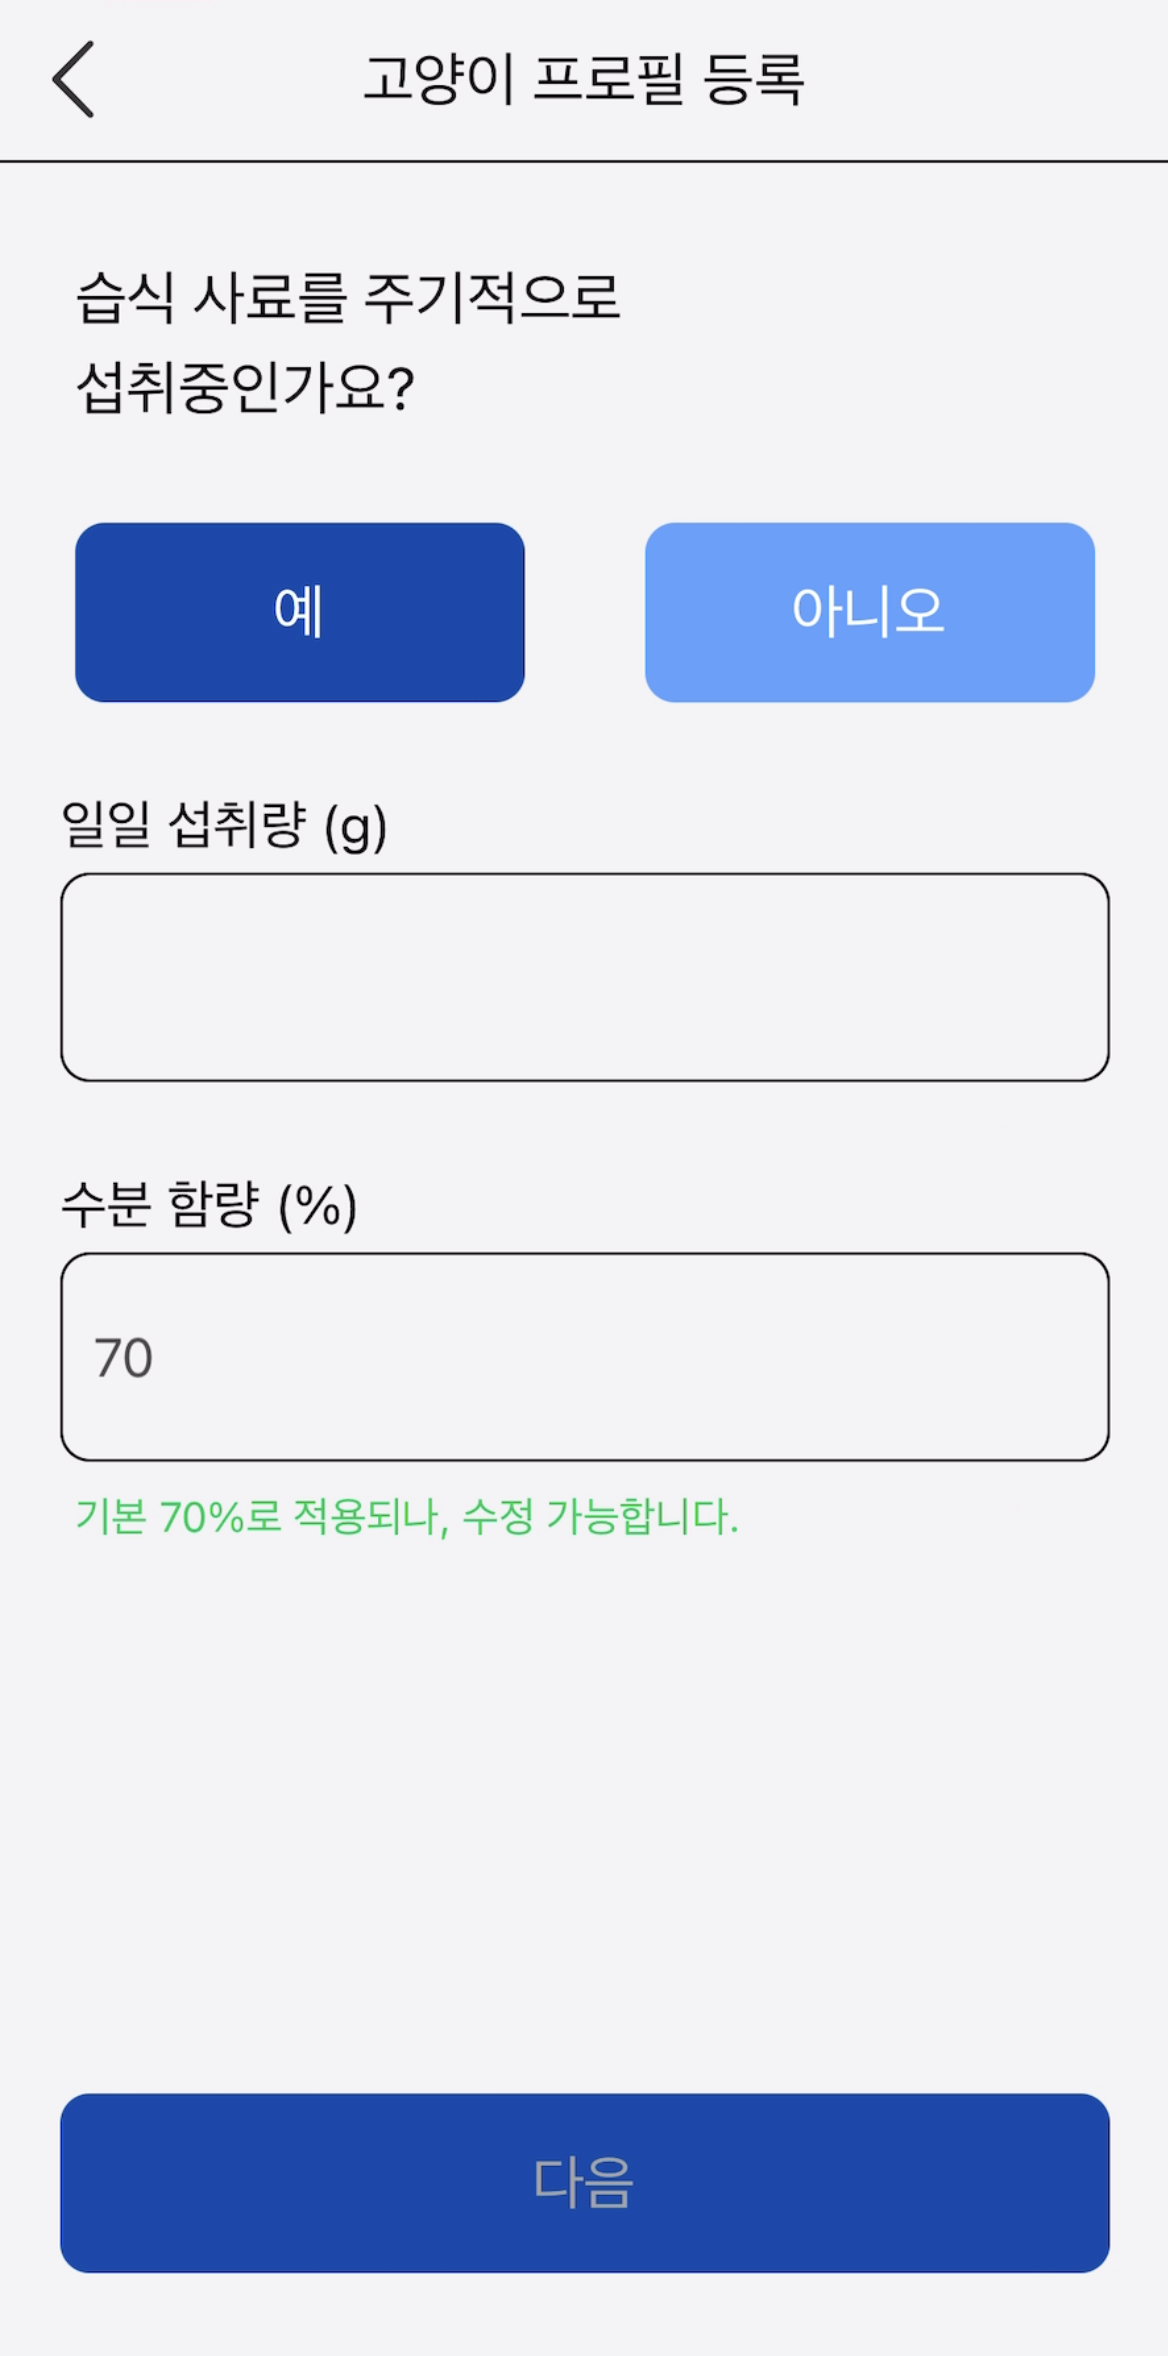
\includegraphics[width=0.27\textwidth]{img/Screen/12_CatFeed.png}
    \item Components Structure of Screen
    \begin{itemize}
        \item TopBar Component
        \item Text Component
        \item Button Component
        \begin{itemize}
            \item Press '예' to display the daily intake and water intake window.
        \end{itemize}
        \item InputContainer Component
        \begin{itemize}
            \item On the CatFeedStuffRegistration screen, a checkEmpty validation is performed only when 'Yes' is pressed.
        \end{itemize}
    \end{itemize}
    \item Flow of Screen
    \begin{itemize}
        \item Press the Go Back button to return to the previous Screen.
        \item Press ‘Yes’ on the intake button and enter daily intake, water content. Then, press Next to save the isEatingFeedStuff, catFeedStuffDailyConsumption and catFeedStuffMoistureContent global variables using the Context API.
        \item Press 'No' and then press 'Next' to store false in the isEatingFeedStuff and 0 in the catFeedStuffDailyConsumption, catFeedStuffMoistureContent.
        \item Next, it goes to the CatHydrationRegistration Screen.
    \end{itemize}
\end{itemize}
\newpage

\subsubsection{CatHydrationRegistration}
\begin{itemize}
    \item[] 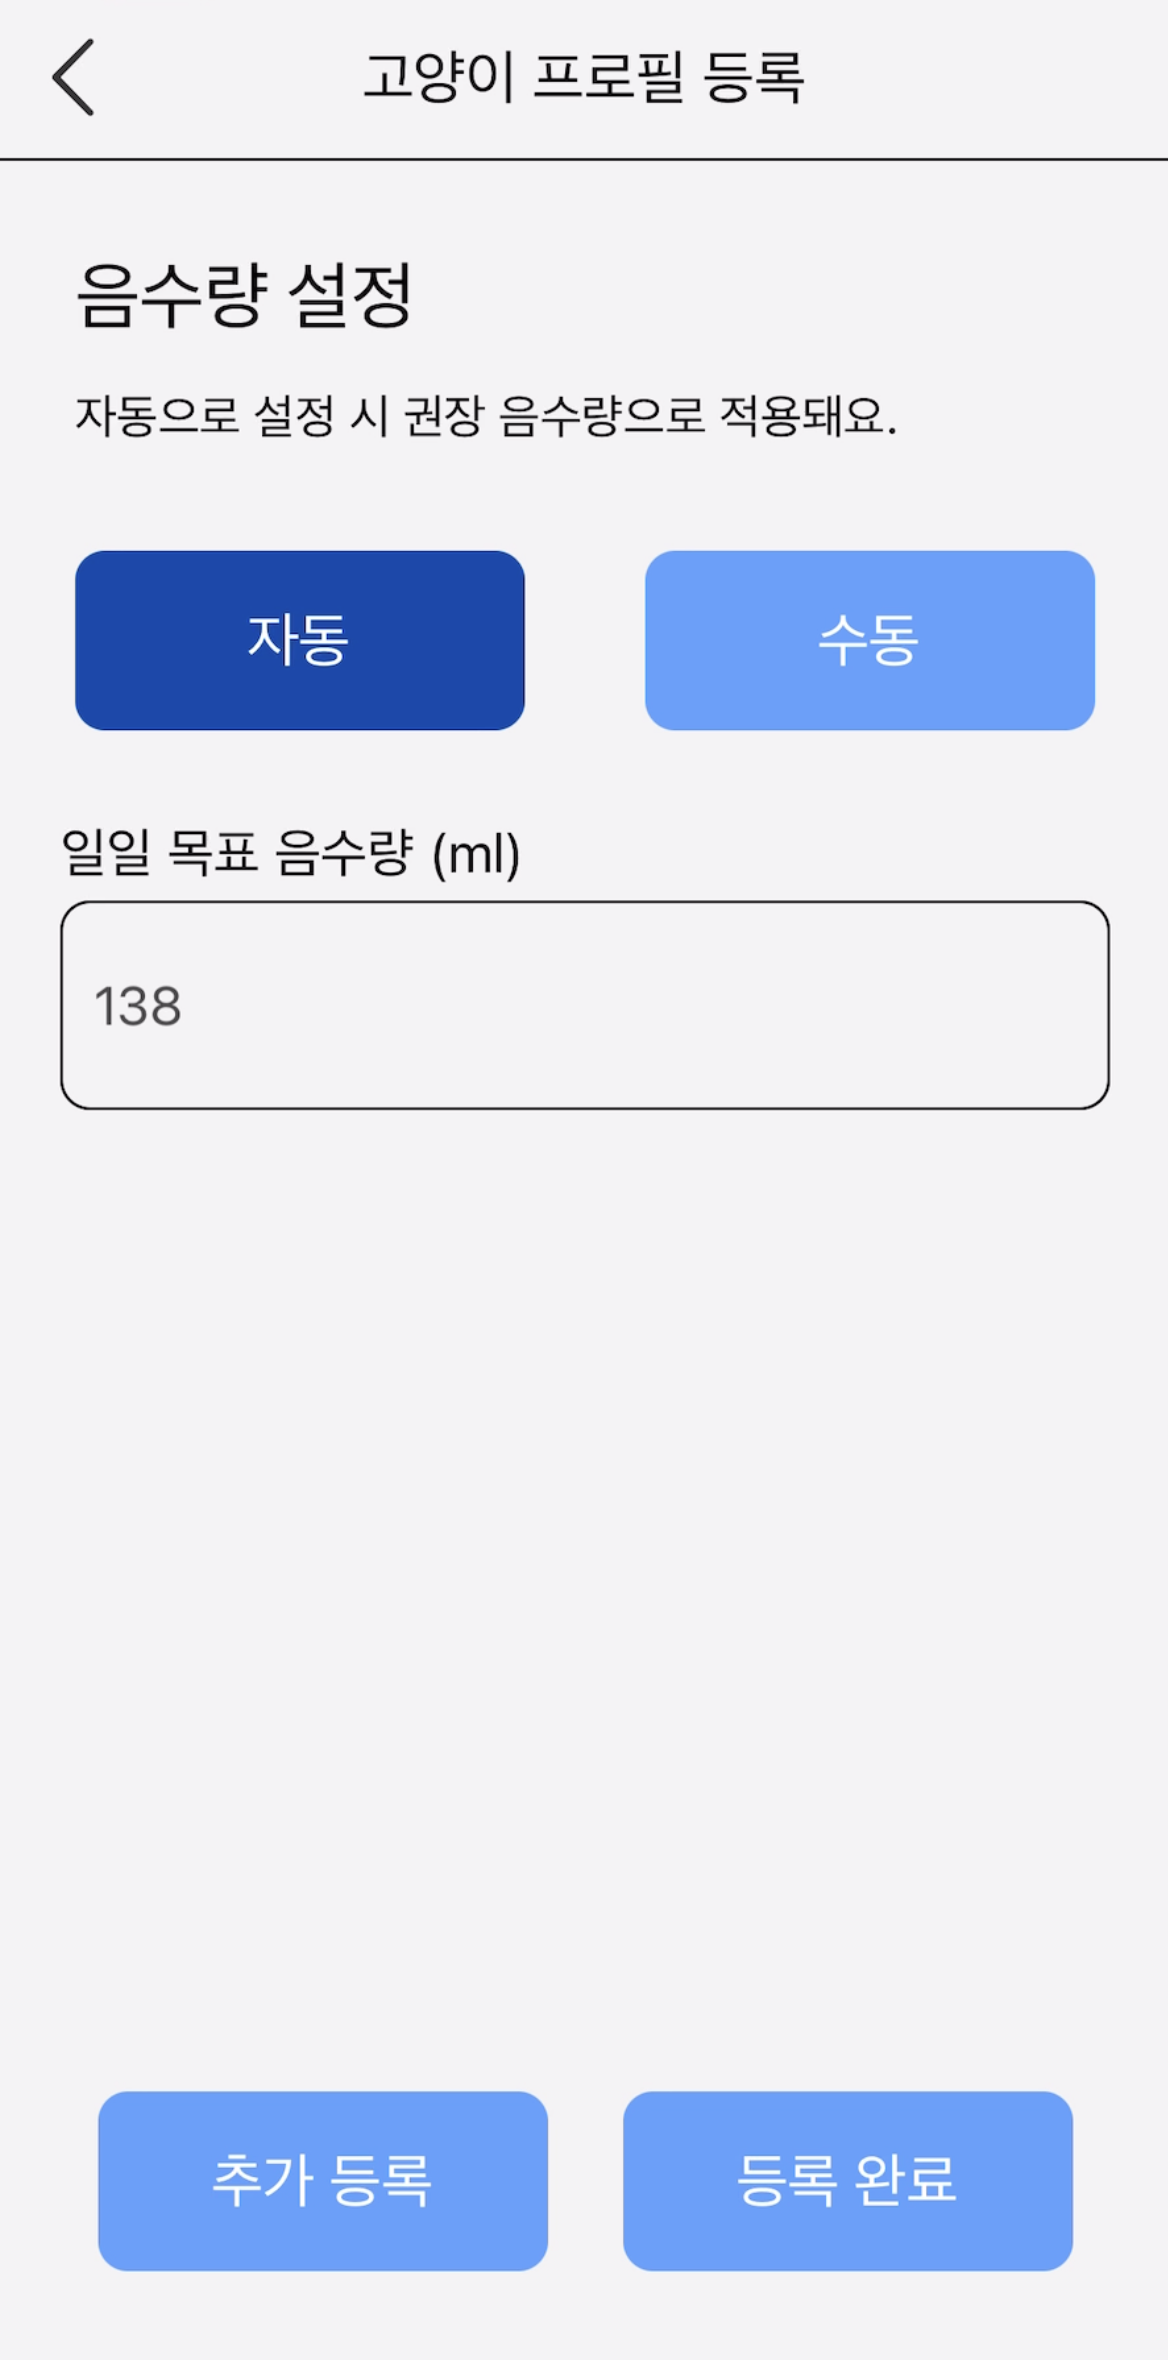
\includegraphics[width=0.27\textwidth]{img/Screen/13_CatHydration.png}
    \item Components Structure of Screen
    \begin{itemize}
        \item TopBar Component
        \item Text Component
        \item Button Component
        \item InputContainer Component
        \begin{itemize}
            \item Press 'Auto' to automatically calculate the recommended water intake and automatically enter it into the input box.
            \item On the CatHyditionRegistration screen, a checkEmpty  validation is only performed.
        \end{itemize}
    \end{itemize}
    \item Flow of Screen
    \begin{itemize}
        \item Press the Go Back button to return to the previous Screen.
        \item Press 'Automatically' on how to set the water intake and then press the 'Additional Registration' or 'Registration Completed' button to store true in the isHyditionAuto global variable with the Context API and substitute the values of the global variable catFeedStuffDailyConsumption, catFeedStuffMoistureContent into the recommended drinking volume formula and store the calculated values in the catGoalHydition global variable.
        \item Press 'Manually' and enter the daily target water intake, then press the 'Additional Registration' or 'Registration Completed' button to store false in the global variable isHydrationAuto and save the input in the global variable catGoalHydration.
        \item Then, call the CatInfoRegist API.
        \item Once you have pressed the 'Additional Register' button, it goes back to the CatProfileRegistration Screen.
        \item If you press the 'Complete Registration' button, delete the global variables' value related to cat information and navigate to the Main screen.\\
    \end{itemize}
\end{itemize}

\subsubsection{Main}
\begin{itemize}
    \item[] 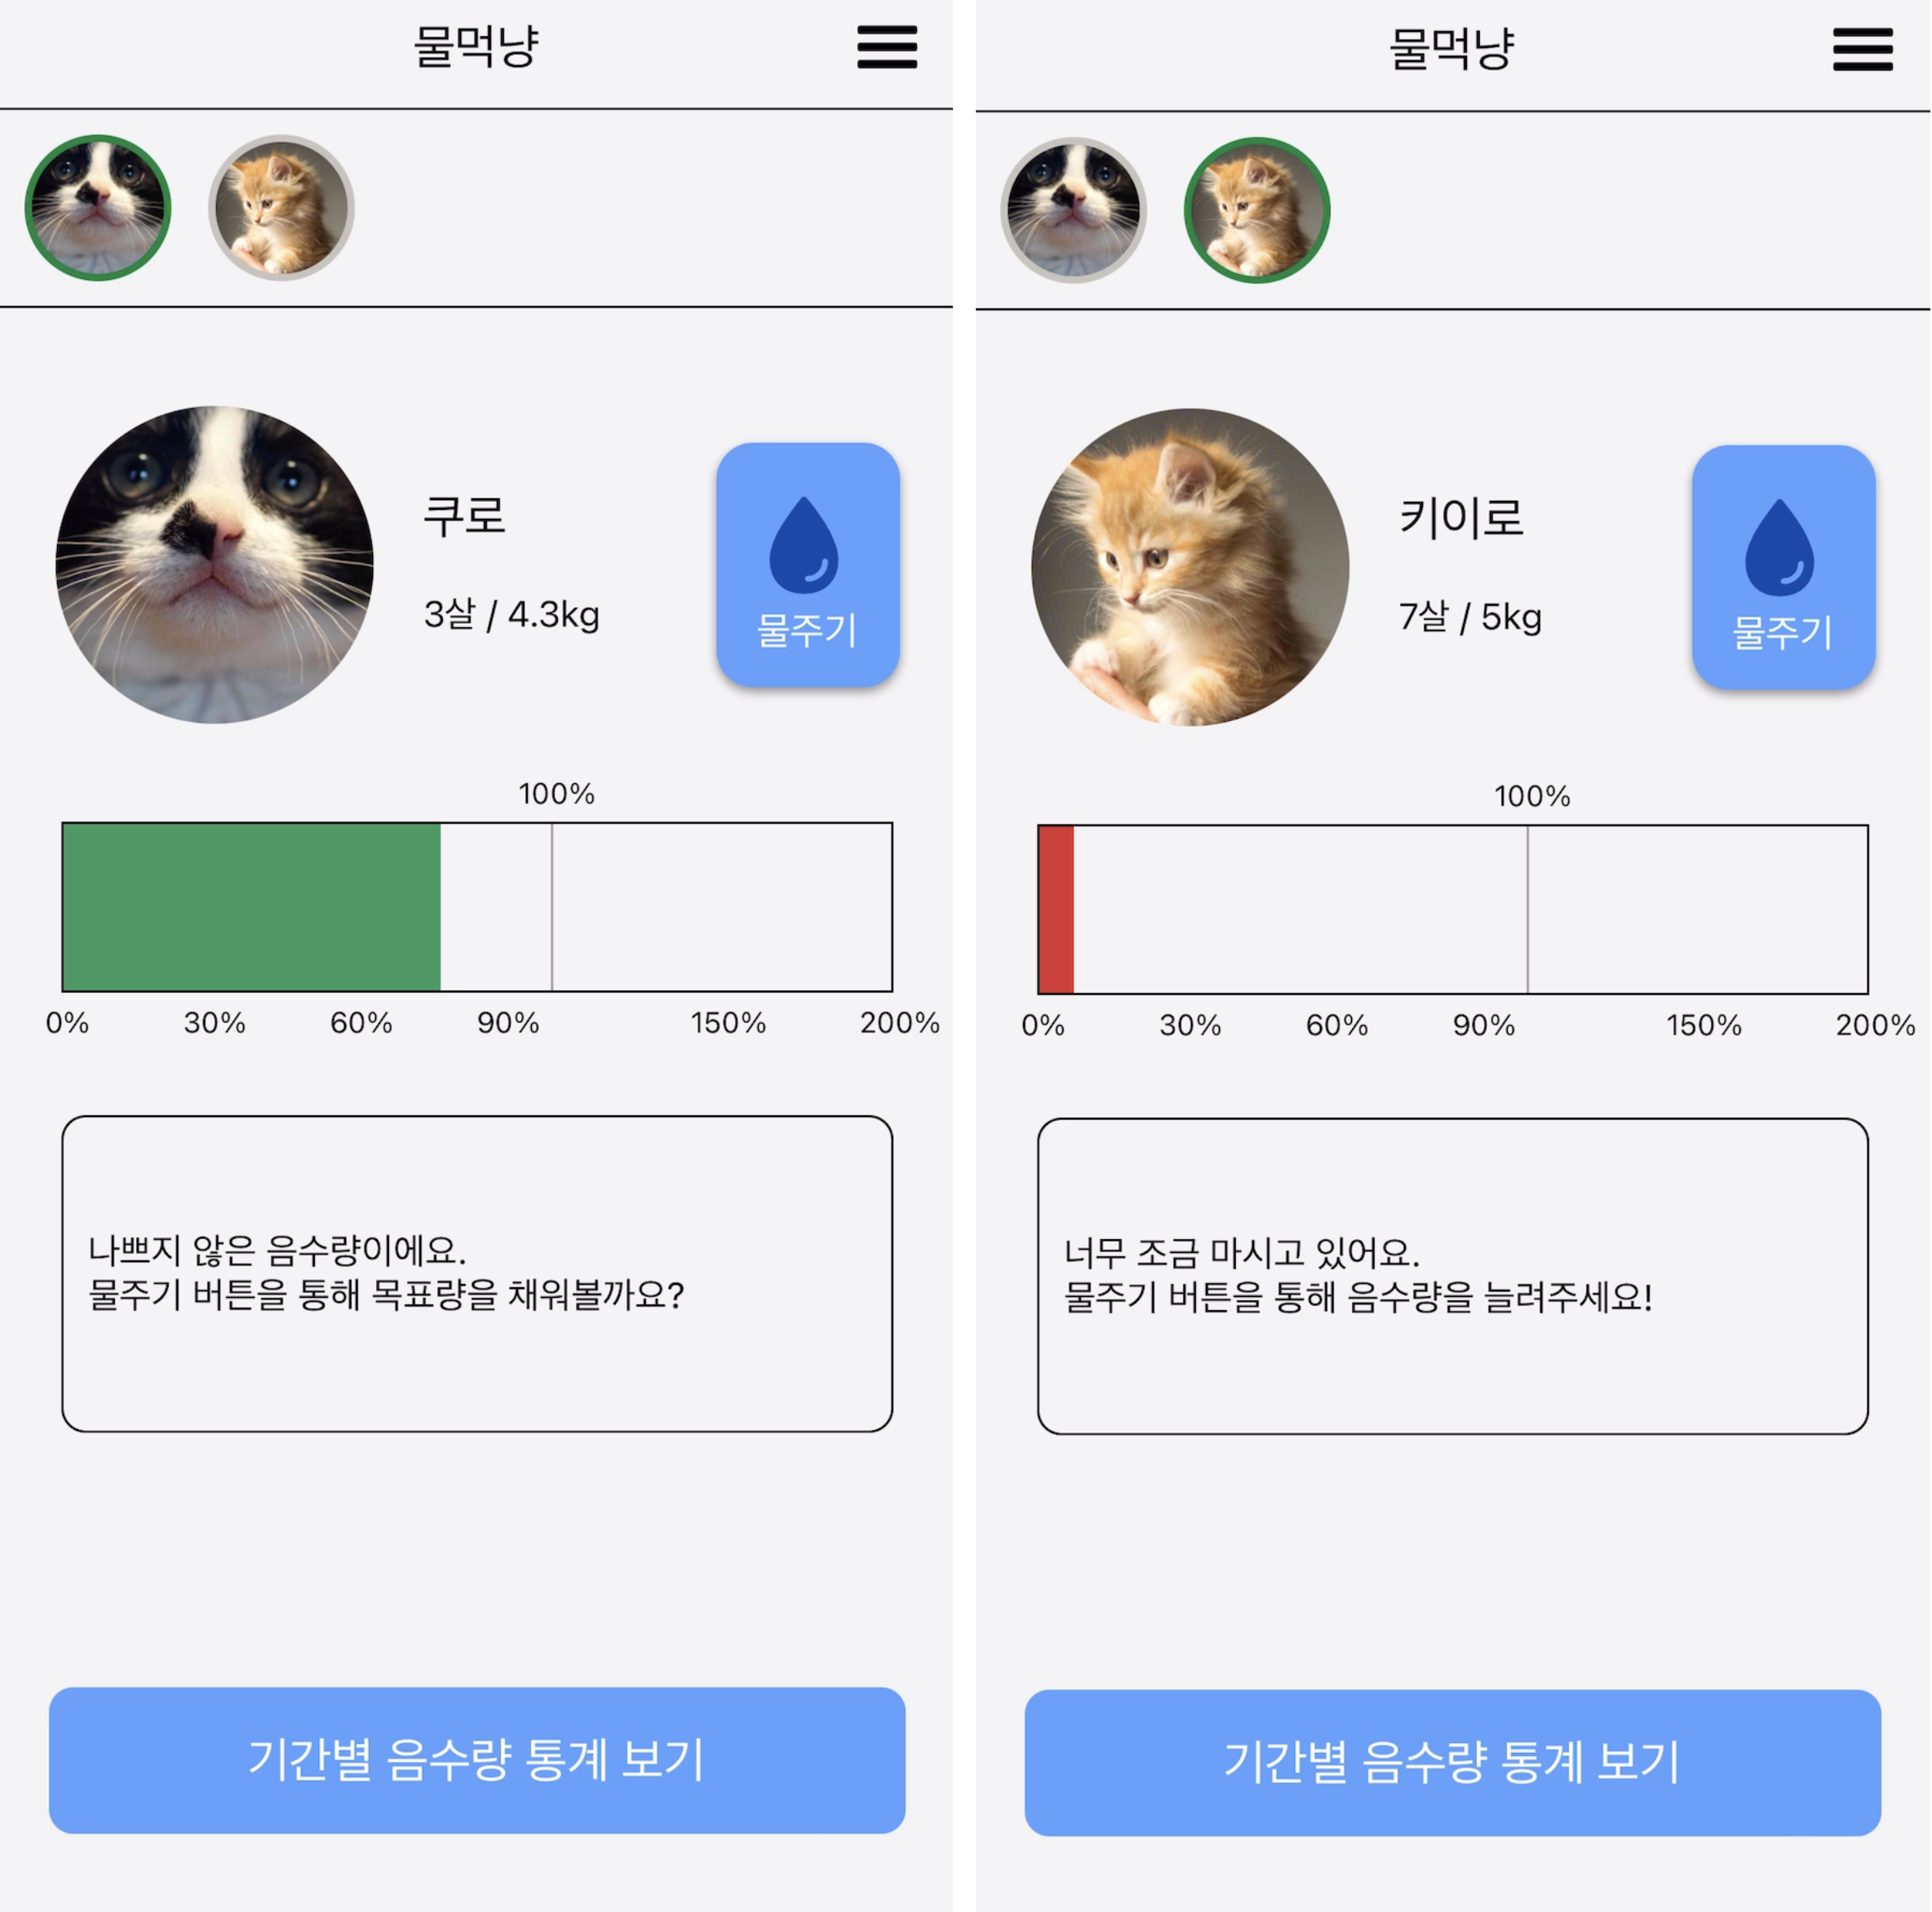
\includegraphics[width=0.45\textwidth]{img/Screen/14_Main.png}
    \item Components Structure of Screen
    \begin{itemize}
        \item TopBar Component
        \item CatProfileList Component
        \item CatProfile Component
        \item HydrationButton Component
        \item HydrationGauge Component
        \begin{itemize}
            \item From 0\% to 29\%: Red
            \item From 30\% to 59\%: Yellow
            \item From 60\% to 89\%: Green
            \item From 90\% to 150\%: Blue
            \item From 151\% to 200\%: Red
        \end{itemize}
        \item EvaluationText Component
        \item Button Component
    \end{itemize}
    \item Flow of Screen
    \begin{itemize}
        \item Call the GetCatProfileList API in the Mount step, process the response, and call the GetCatMainInfo API.
        \item Press the menu button to open the Drawer.
        \item In the cat profile list at the top, call the GetCatMainInfo API whenever user press a picture of another cat profile that is not currently selected.
        \item A water intake gauge shows how much the cat has intaken today so far.
        \item Different assessments appear depending on the gauge.
        \item Press the 'View period-based hydrration statistics' button to go to the Hydration Statistics Screen.
    \end{itemize}
\end{itemize}
\newpage

\subsubsection{HydrationStatistics}
\begin{itemize}
    \item[] 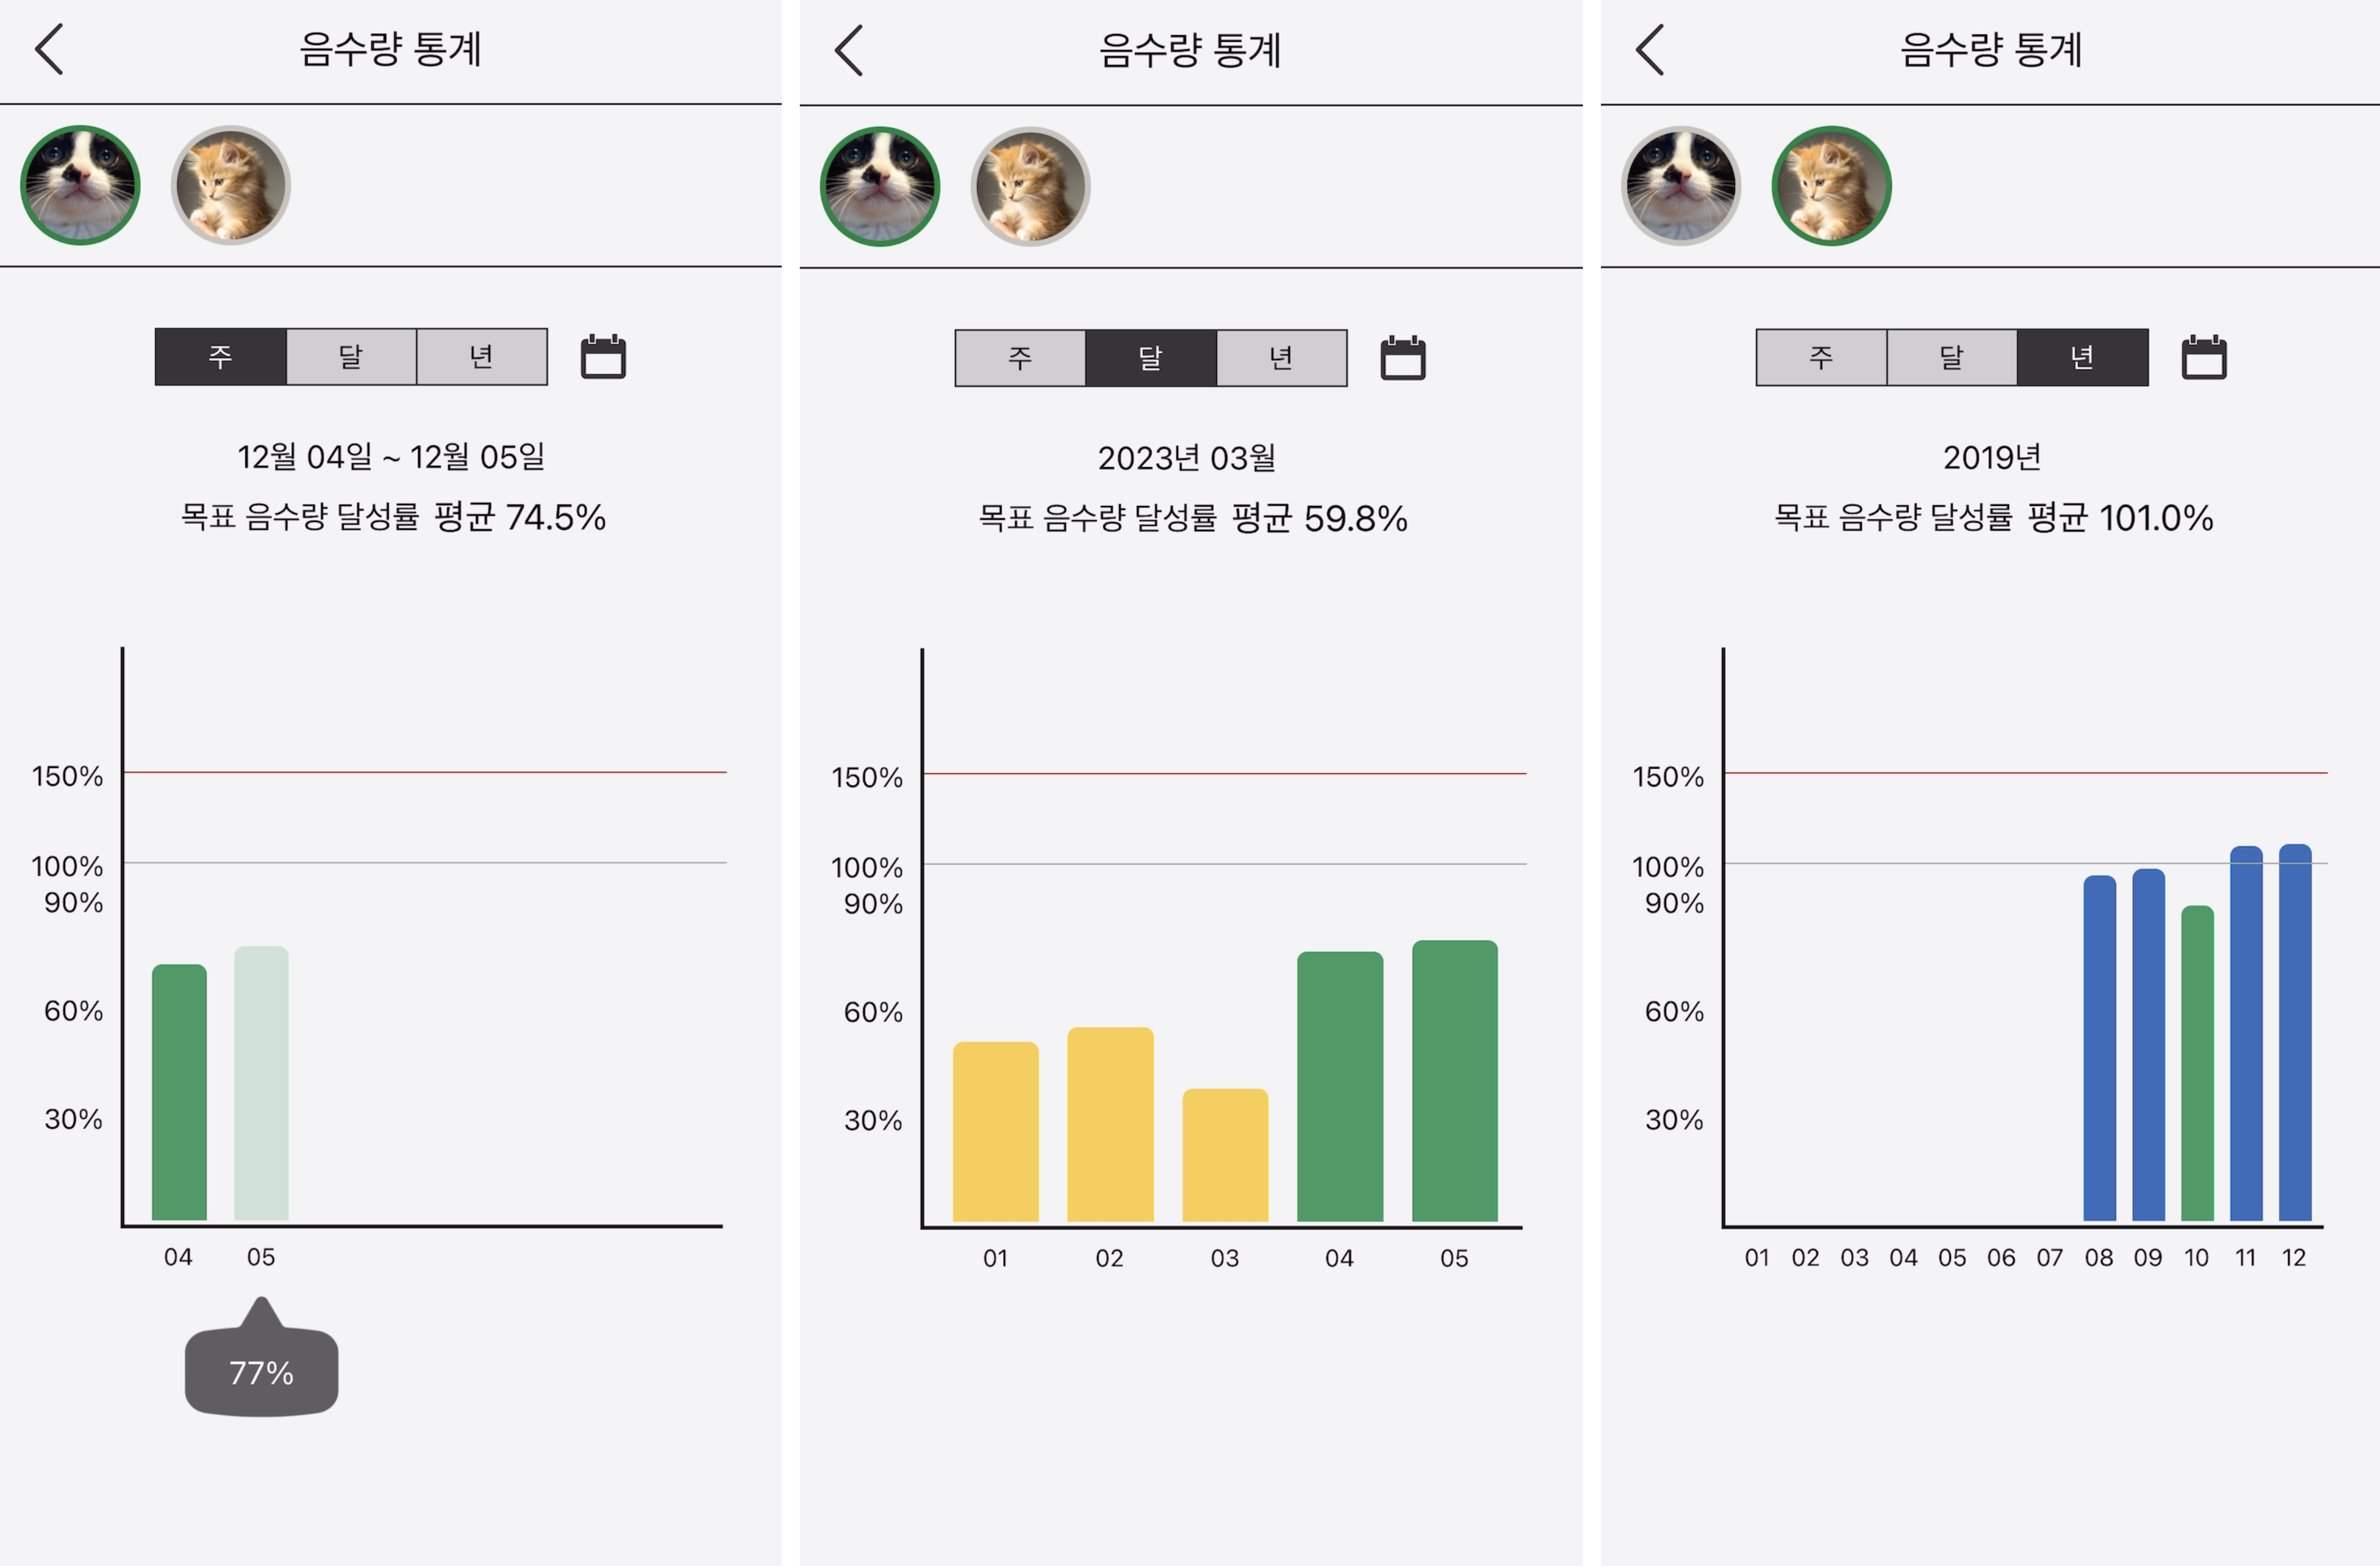
\includegraphics[width=0.45\textwidth]{img/Screen/15_StatisticsGraph.png}
    \item Components Structure of Screen
    \begin{itemize}
        \item TopBar Component
        \item CatProfileList Component
        \item UnitSelect Component
        \item Calender Component
        \item[] 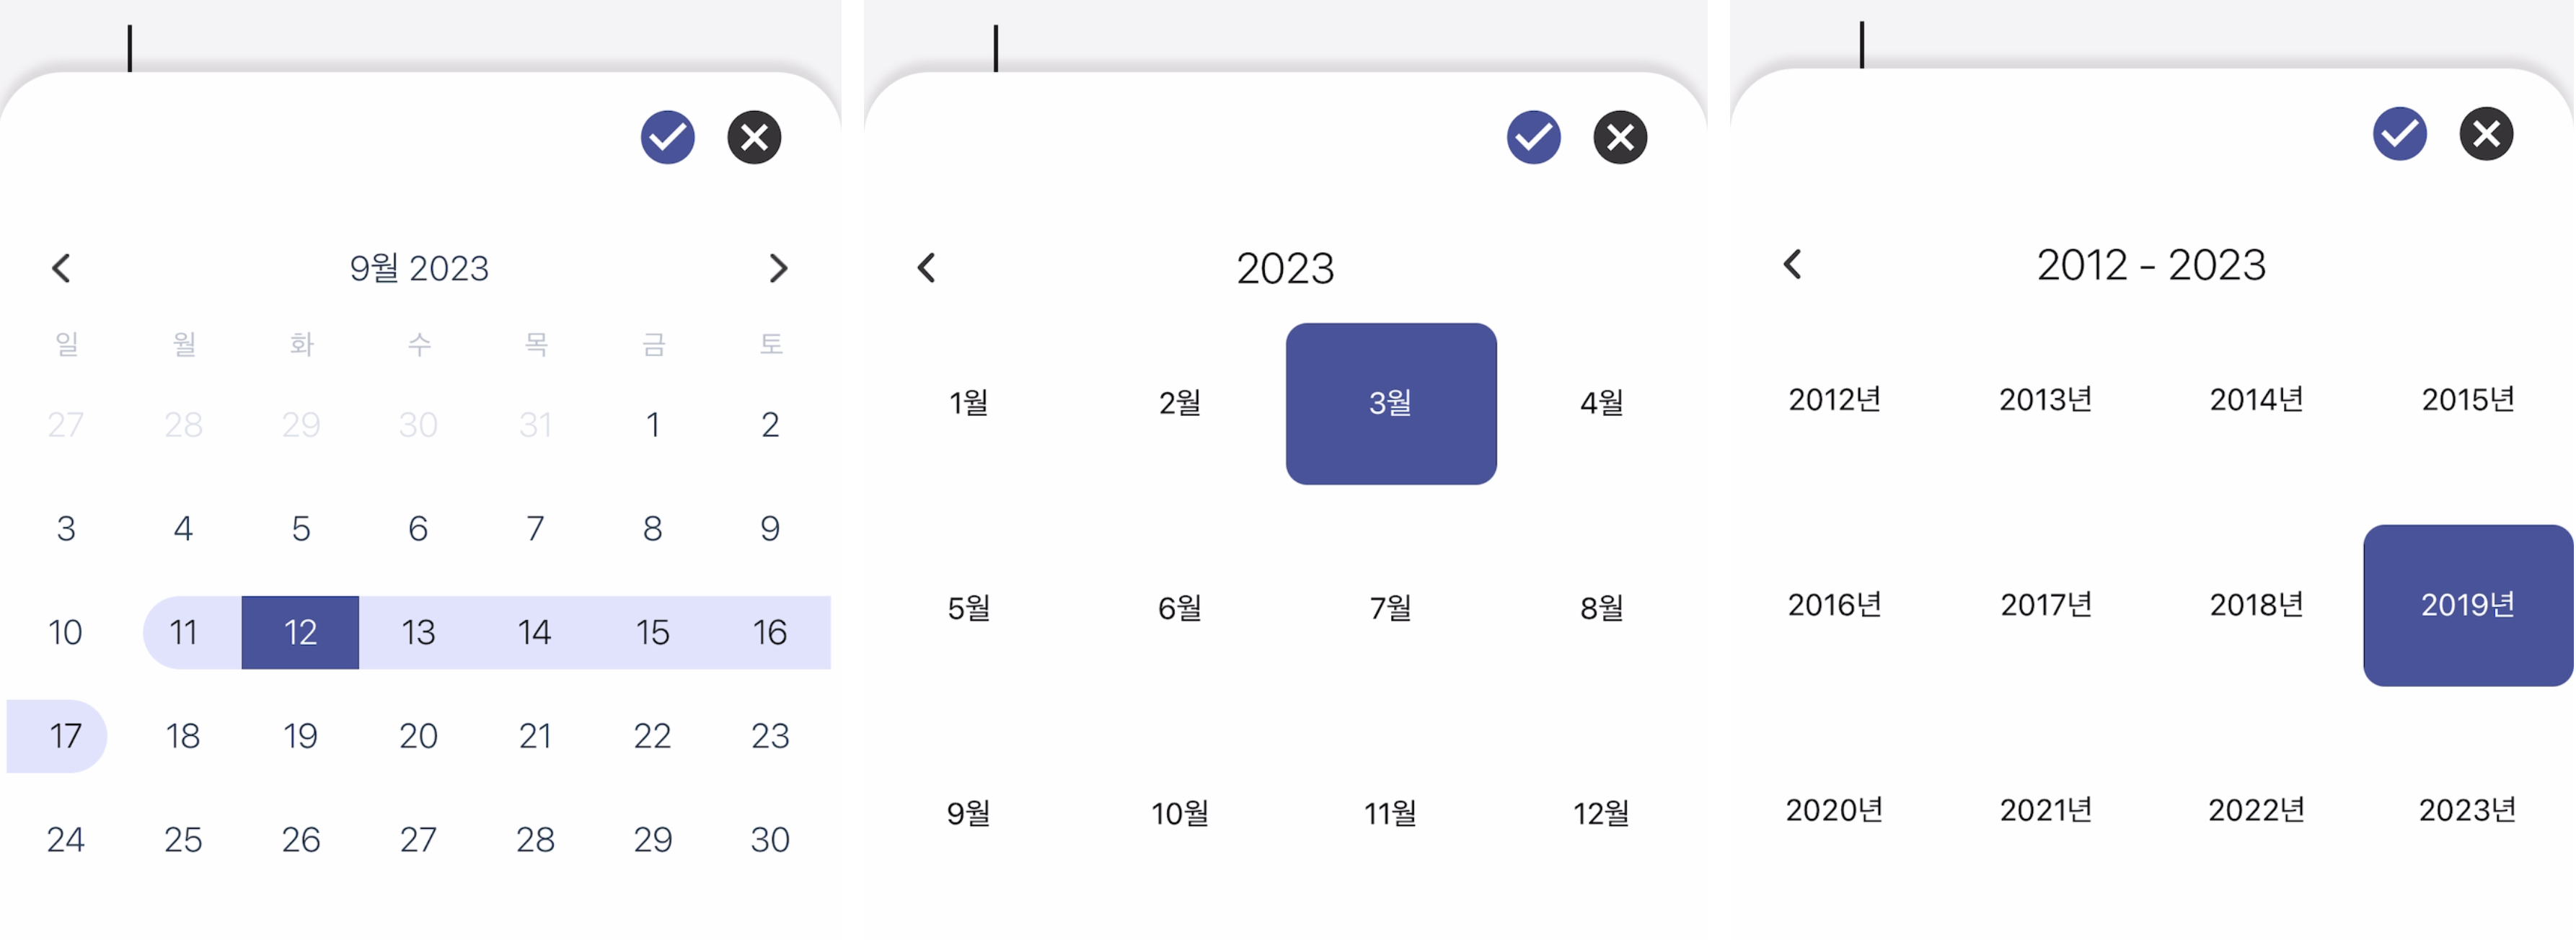
\includegraphics[width=0.42\textwidth]{img/Screen/16_StatisticsCalendar.png}
        \item AvgText Component
        \item HydrationGraph Component
        \begin{itemize}
            \item XAndBar Component
        \end{itemize}
    \end{itemize}
    \item Flow of Screen
    \begin{itemize}
        \item GetCatStatistics API is called in the Mount step.
        \item Press the Go Back button to return to the previous Screen.
        \item From the cat profile list at the top, whenever you click cat's picture that is not currently selected, change the statistical period, or select a specific week/month/year in the calendar, GetCatStatistics API is called.
        \item For 'Week', if you select a specific date in the calendar, the week containing that date is selected.
        \item Touch a particular bar to display specific figures.
    \end{itemize}
\end{itemize}
\newpage

\subsubsection{Drawer}
\begin{itemize}
    \item[] 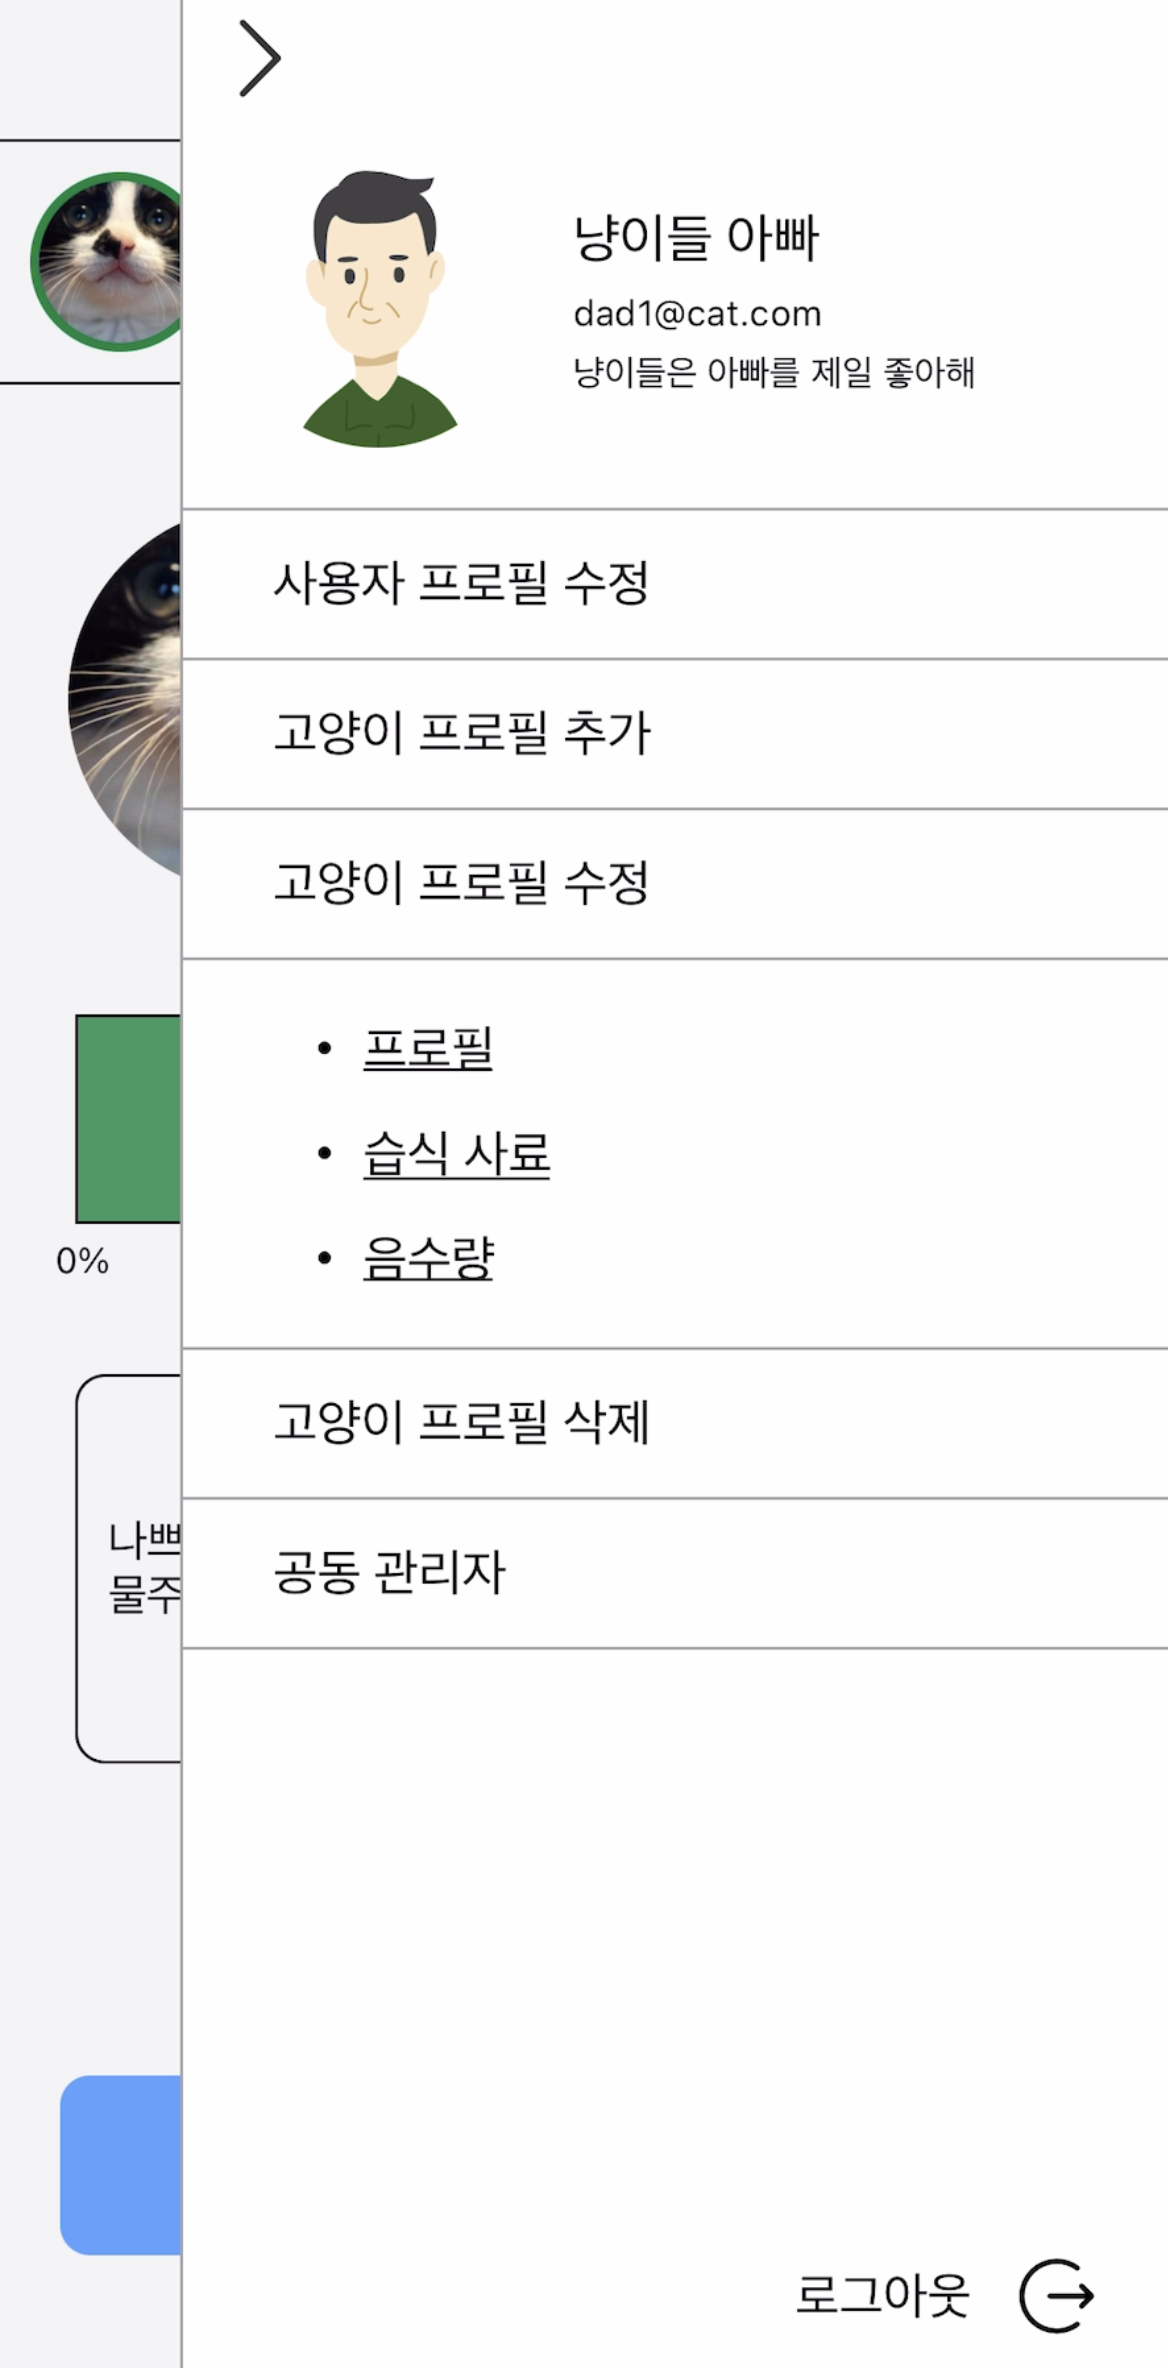
\includegraphics[width=0.27\textwidth]{img/Screen/17_Drawer.png}
    \item Components Structure of Screen
    \begin{itemize}
        \item TopBar Component
        \item UserProfile Component
        \item DrawerRoute Component
        \item SubDrawerRotue Component
        \item LogoutButton Component
        \item SelectCatAlert Component
        \begin{itemize}
            \item[] 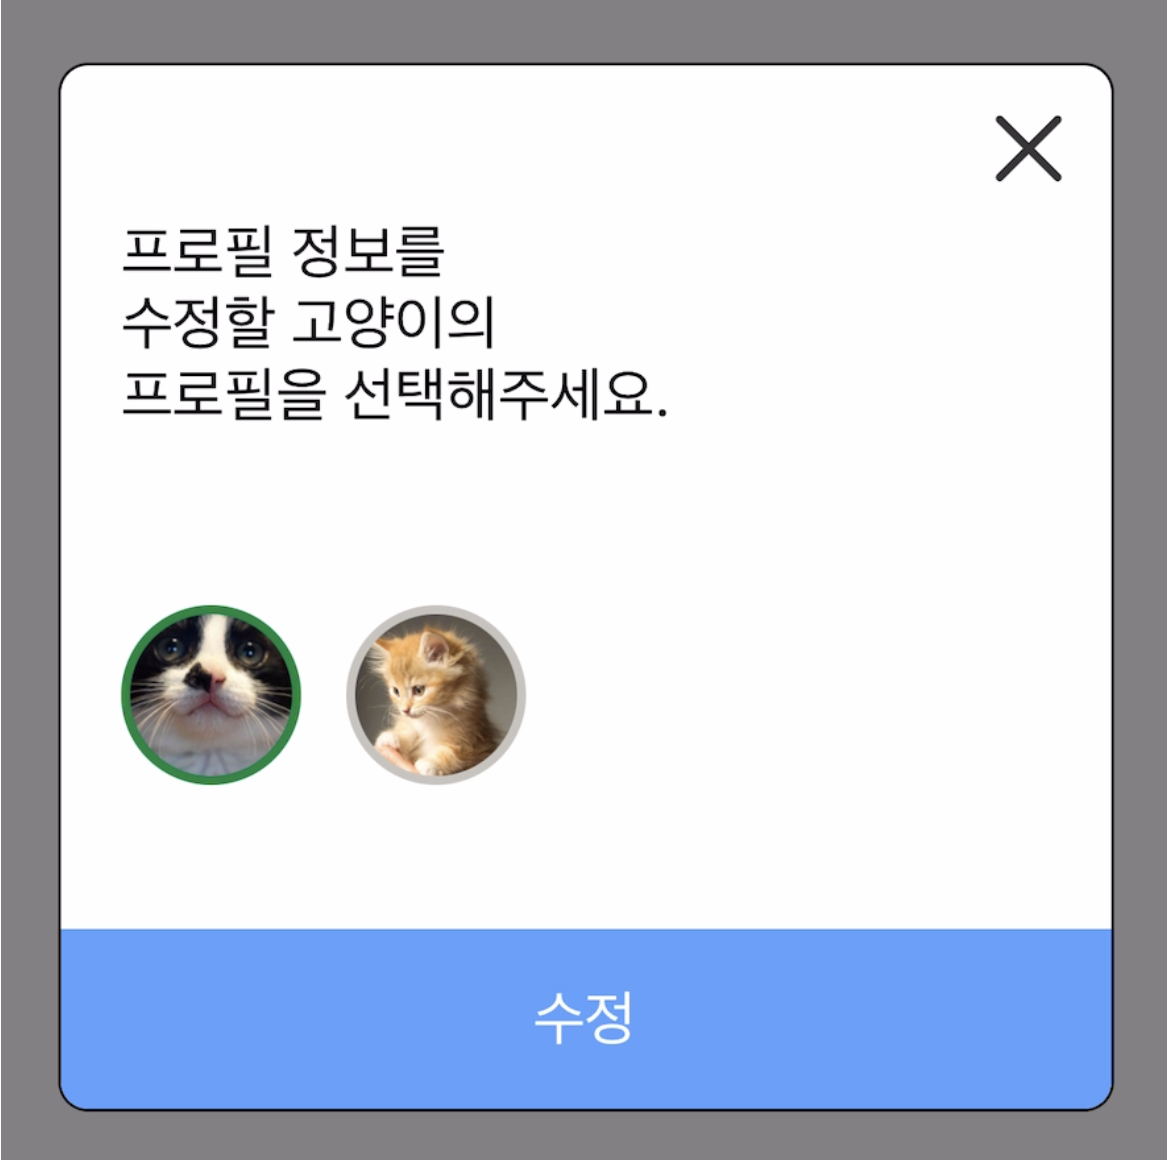
\includegraphics[width=0.27\textwidth]{img/Screen/18_CatAlert.png}
            \item IconButton Component
            \item Title Component
            \item Text Component
            \item CatProfileList Component
            \item Button Component
        \end{itemize}
    \end{itemize}
    \item Flow of Screen
    \begin{itemize}
        \item Press the Close button to close the Drawer.
        \item Press the 'Modify User Profile' button to go to the UserProfileModification Screen.
        \item Press the 'Add Cat Profile' button to go to the CatProfileRegistration Screen.
        \item Pressing the 'Profile', 'Wet Food', and 'Hydration' buttons under 'Modify Cat Profile' displays SelectCatAlert to select the cat to modify the information.
        \item Select the cat you want to modify and press the 'Modify' button to go to the Cat\_\_\_\_\_Modification Screen.
        \item When you press the 'Delete Cat Profile' button, a SelectCatAlert Component will appear to select the cat to delete all the information.
        \item Select the cat you want to delete and press the 'Delete' button to call the DeleteCatInfo API.
        \item Press the 'Co-Manager' button to navigate to the CoManager Screen.
        \item If user presses the Logout button, the Logout API is called.\\
    \end{itemize}
\end{itemize}

\subsubsection{UserProfileModification}
\begin{itemize}
    \item Components Structure of Screen
    \begin{itemize}
        \item Identical to UserProfileRegistration Screen.
    \end{itemize}
    \item Flow of Screen
    \begin{itemize}
        \item Call the GetUserProfile API in the Mount step.
        \item Call the ModifyUserProfile API when the 'Modify' button is pressed.
        \item The rest is the same as the UserProfileRegistration Screen.\\
    \end{itemize}
\end{itemize}

\subsubsection{CatProfileModification}
\begin{itemize}
    \item Components Structure of Screen
    \begin{itemize}
        \item Identical to CatProfileRegistration Screen.
    \end{itemize}
    \item Flow of Screen
    \begin{itemize}
        \item Call the GetCatProfile API in the Mount step.
        \item Call the ModifyUserProfile API when the 'Modify' button is pressed.
        \item The rest is the same as the CatProfileRegistration Screen.\\
    \end{itemize}
\end{itemize}

\subsubsection{CatFeedStuffModification}
\begin{itemize}
    \item Components Structure of Screen
    \begin{itemize}
        \item Identical to CatFeedStuffRegistration Screen.
    \end{itemize}
    \item Flow of Screen
    \begin{itemize}
        \item Call the GetCatFeedStuffAPI in the Mount step.
        \item Call the ModifyCatFeedStuff API when the 'Modify' button is pressed.
        \item The rest is the same as the CatFeedStuffRegistration Screen.\\
    \end{itemize}
\end{itemize}

\subsubsection{CatHydrationModification}
\begin{itemize}
    \item Components Structure of Screen
    \begin{itemize}
        \item Identical to CatHydrationRegistration Screen.
    \end{itemize}
    \item Flow of Screen
    \begin{itemize}
        \item Call the GetCatHydration in the Mount step.
        \item Call the ModifyCatHydration API when the 'Modify' button is pressed.
        \item The rest is the same as the CatHydrationRegistration Screen.\\
    \end{itemize}
\end{itemize}

\subsubsection{CoManager}
\begin{itemize}
    \item[] 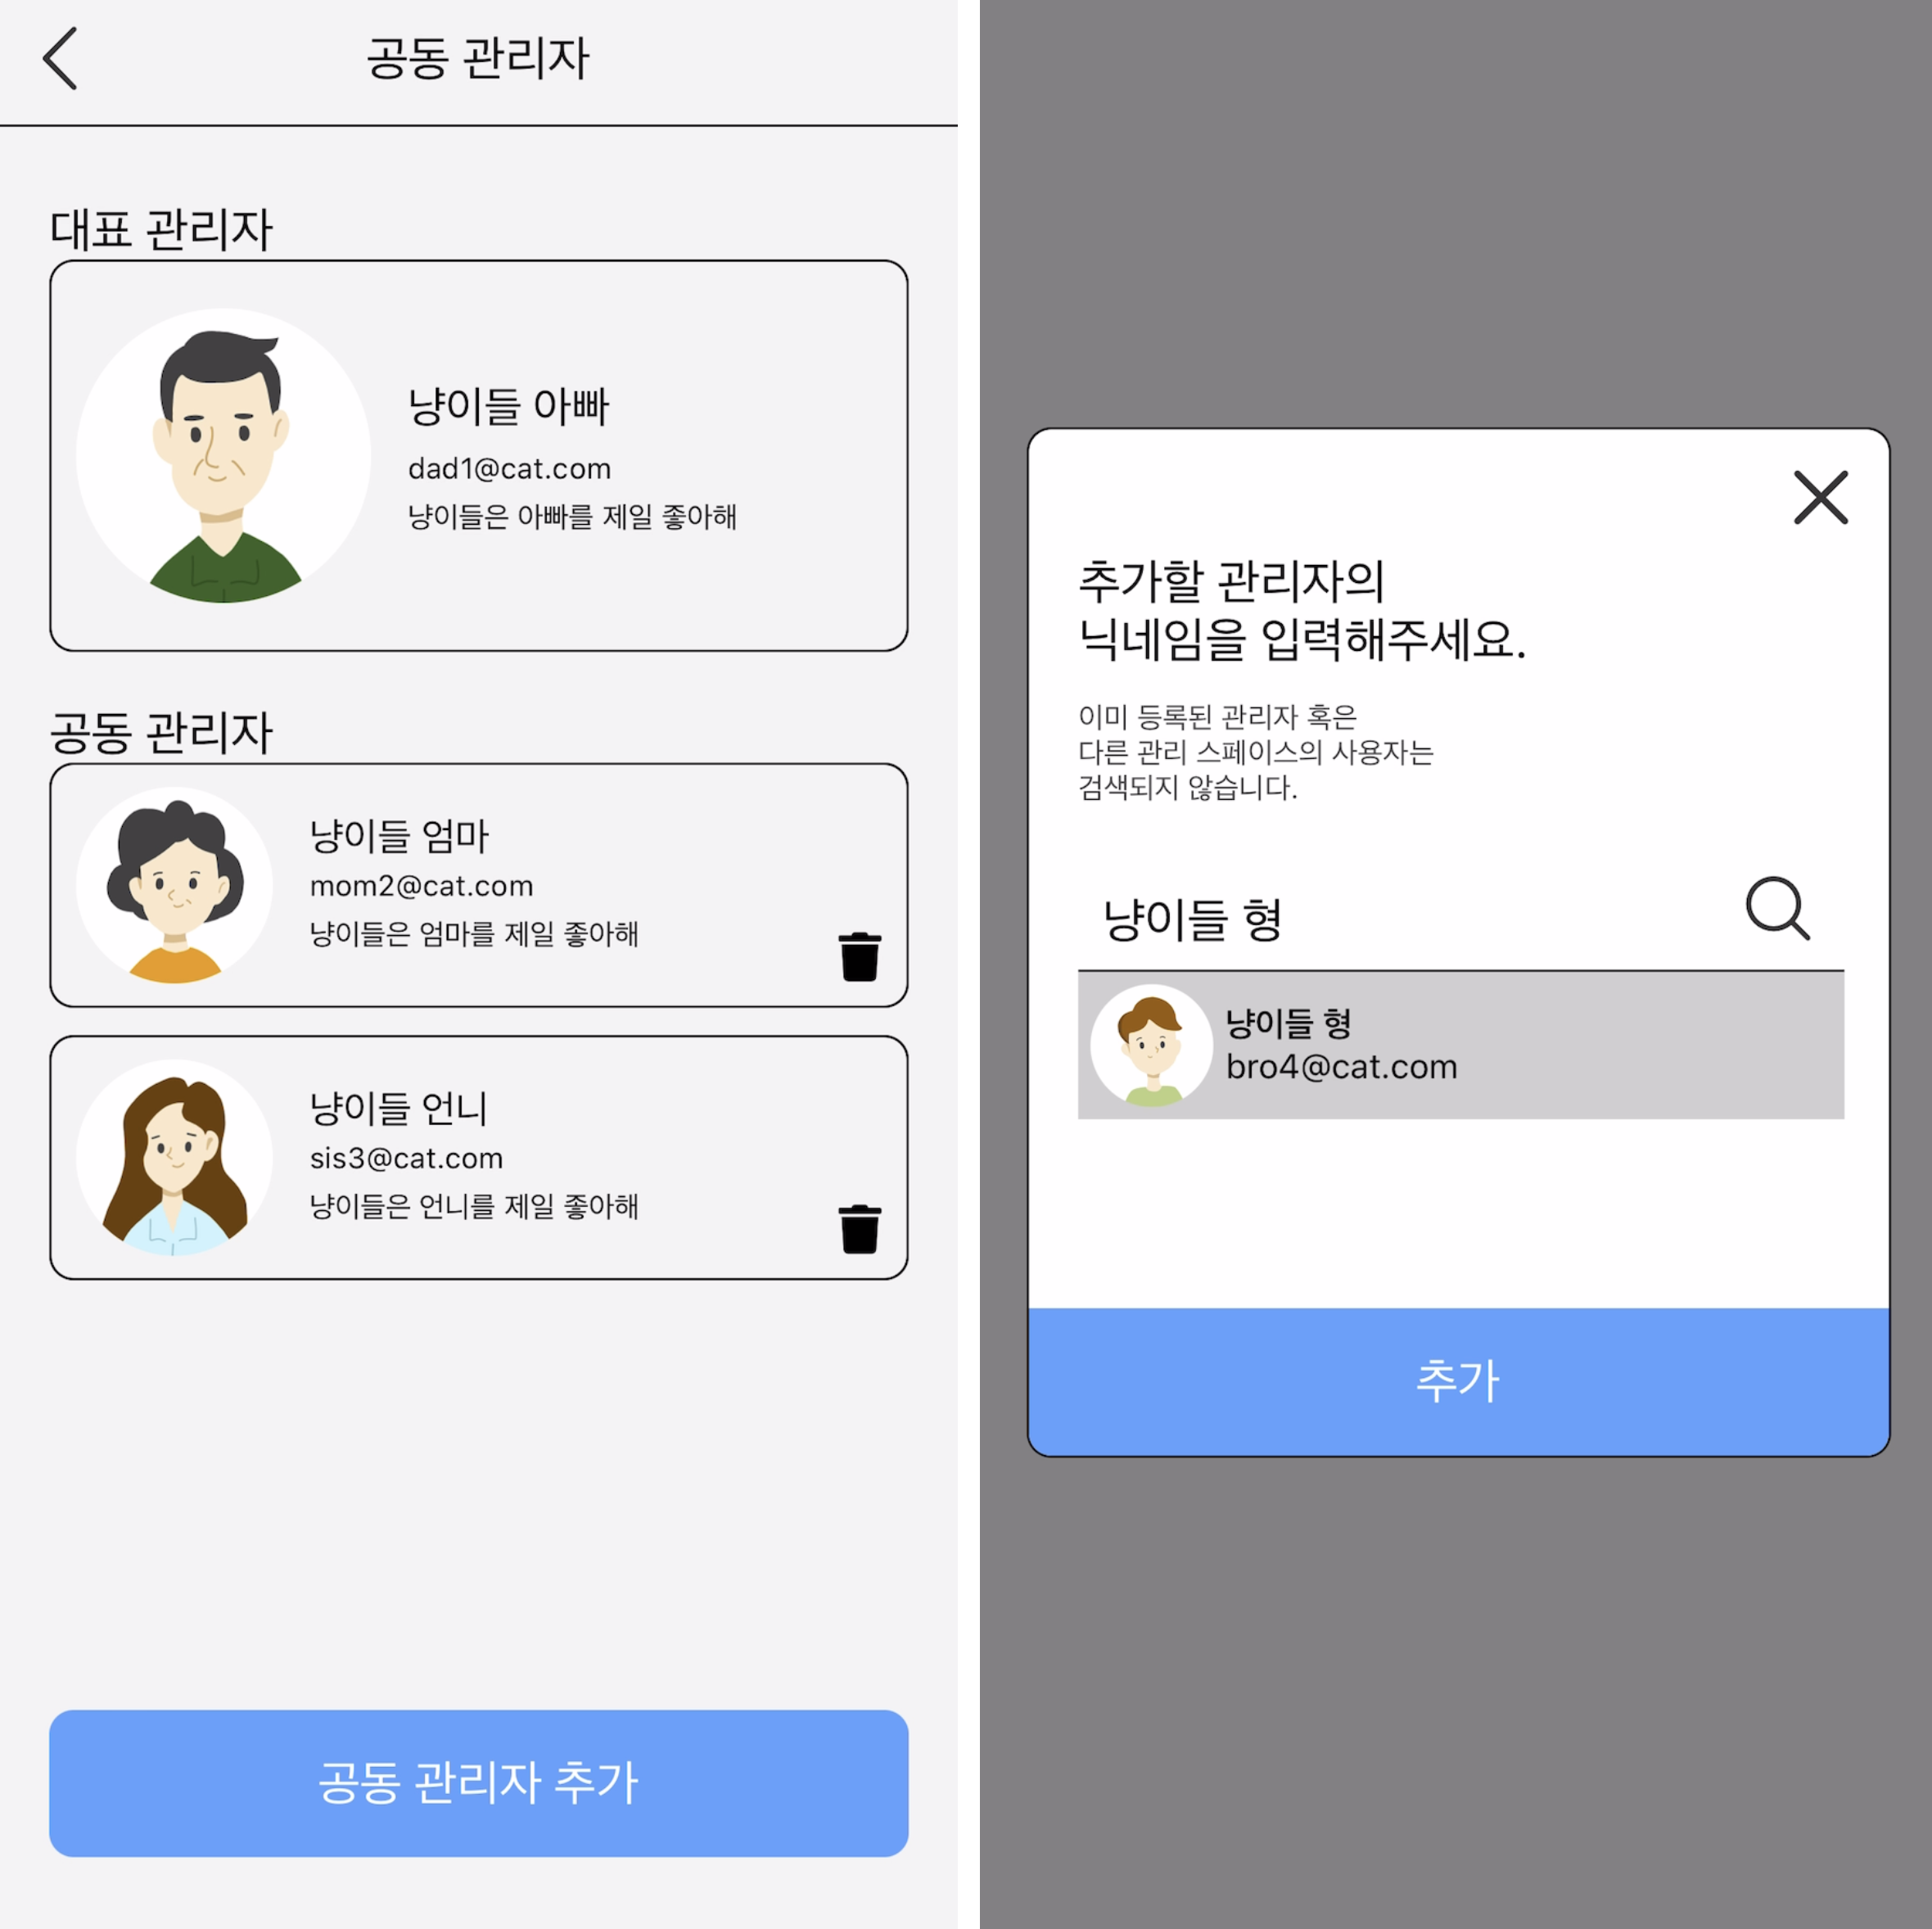
\includegraphics[width=0.45\textwidth]{img/Screen/19_CoManager.png}
    \item Components Structure of Screen
    \begin{itemize}
        \item TopBar Component
        \item ManagerCard Component
        \item Button Component
        \item SearchUserAlert Component
        \begin{itemize}
            \item IconButton Component
            \item Title Component
            \item Text Component
            \item Search Component
            \item SearchedUser Component
            \item Button Component
        \end{itemize}
        \item Alert Component
    \end{itemize}
    \item Flow of Screen
    \begin{itemize}
        \item Call the GetManagerList API in the Mount step.
        \item Pressing the Add Administrator button to displays the SearchUserAlert Component. After entering a nickname and when you press the search icon, it calls the UserSearch API.
        \item When pressing the 'Add Co-Manager' button, the SearchUserAlert Component appears. After entering a nickname and clicking the search icon, it triggers the User Search API. Pressing the 'Add' button thereafter calls the AddCoManager API.
        \item On the Administrator Screen, the Trash icon appears in the Co Manager Card, and when you press the 'Yes' button in the Manager Delete Alert Component, the DeleteCoManager API is called.
        \\
    \end{itemize}
\end{itemize}

\newpage
\subsection{BackEnd API Usage Logic}
\subsubsection{AutoLogin API}
\begin{itemize}
    \item Client send HTTP Request to Server
    \begin{itemize}
        \item Auto Login Case 1) Users with auto login disabled
        \begin{itemize}
            \item Set the userEmail value to HTTP Request and send the Request(POST) to the Server.
        \end{itemize}
        \item Auto Login Case 2) Users with auto login enabled
        \begin{itemize}
            \item Set the session that contains the Session ID in the AysncStorage to HTTP Request(GET) and send the request to the Server.
            \\
        \end{itemize}
    \end{itemize}
    \item HTTP Request process in the sever, HTTP Response from server to client
    \begin{itemize}
        \item Auto Login Case 1) Users with auto login disabled
        \begin{itemize}
            \item If the value set in the HTTP Request is userEmail, generate a sessionID and add a record along with userEmail to the session table.
            \item When querying the record in the user table with userEmail, if there is a value for management\_space\_id, it is saved in the variable managementSpaceId, and if not, it is saved as null.
            \item Set managementSpaceId, and SessionId in HTTP Response to send a response to the Client.
        \end{itemize}
        \item Auto Login Case 2) Users with auto login enabled
        \begin{itemize}
            \item The session ID stored in the session set in the HTTP Request inquires the record in the session table and stores the user\_email value in the userEmail variable.
            \item When querying the record in the user table with userEmail, if there is a value for management\_space\_id, it is saved in the variable managementSpaceId, and if not, it is saved as null.
            \item Set userEmail, managementSpaceId to HTTP Response and send a response to the Client.
            \\
        \end{itemize}
    \end{itemize}
    \item HTTP Response Processing in Client side
    \begin{itemize}
        \item The userEmail value set in the HTTP Response is stored as a global variable userEmail using the Context API, and if the managementSpaceId value is not null, it is also stored as a global variable managementSpaceId.
        \item If the sessionID is set in HTTP Response, it saves the cookie in the AsyncStorage before moving into the screen.
        \item If the user have a managementSpaceId value, go to the Main screen, and if the value is null, go to the HowToGoSpace screen.
        \\
    \end{itemize}
\end{itemize}

\subsubsection{Login API}
\begin{itemize}
    \item HTTP Request From Client to Server
    \begin{itemize}
        \item Set userEmail, userPw, and autoLogin values to HTTP Request(POST) and send a request to the server.
        \\
    \end{itemize}
    \item HTTP requests process in Server, HTTP Response from Server to Client
    \begin{itemize}
        \item Case 1) Registered User
        \begin{itemize}
            \item With the userEmail and userPw values set in the HTTP Request, look up the record in the user table. If there is a registered user, store true in the userExists variable and if not, store false.
            \item If the record has user\_nickname and management\_space\_id values, store them in the userNickname and managementSpaceId variables, respectively, and if not, store null.
            \item Case 1-1) Who checked the Auto Login check box
            \begin{itemize}
                \item If the userNickname value is available, and the AutoLogin value set in the HTTP Request is true, the userEmail value is set in the HTTP Request and the request is sent to the Auto Login Case 1 API.
                \item The SessionID set in the HTTP Response transmitted from the Auto Login API is stored in the variable.
                \item If the userNickname value is null and AutoLogin value is true, store null in sessionID variable.
                \item Set userEmail, userNickname, managementSpaceId, and Cookie in HTTP Response to send a response to the Client.
            \end{itemize}
            \item Case 1-2) Users who did not check the Auto Login check box
            \begin{itemize}
                \item If the AutoLogin value set in the HTTP Request is false, set userEmail, userNickname, and managementSpaceId to HTTP Response and send a response to the Client.
            \end{itemize}
        \end{itemize}
    \end{itemize}
    \begin{itemize}
        \item Case 2) Unregistered User
        \begin{itemize}
            \item If the userExists value is false, set the userExists value to HTTP Response and send a response to the Client.
            \\
        \end{itemize}
    \end{itemize}
    \item HTTP Response process in Client side
    \begin{itemize}
        \item Case 1) Registered User
        \begin{itemize}
            \item If userEmail is set in HTTP Response, the userEmail value is saved as a global variable userEmail using the Context API.
            \item Check whether there is a set userNickname value in HTTP Response or null.
            \item The existence of the userNickname value means that the user profile has been registered.
            \item Case 1-1) User that has completed profile registration
            \begin{itemize}
                \item If the managementSpaceId value set in HTTP Response is not null, it is stored as a global variable managementSpaceId.
                \item If the sessionID is set in HTTP Response, store the sessionID in the  AsyncStorage.
                \item Then, if the user has a managementSpaceId value, it moves to the Main screen, and if the value is null, it moves to the HowToGoSpace screen.
            \end{itemize}
            \item Case 1-2) User who needs to register user profile
            \begin{itemize}
                \item If the userNickname value is null, display an Alert Component that says "자동 로그인 설정은 사용자 프로필 등록을 한 다음 사용이 가능합니다." and navigate to the UserProfileRegistration screen.
            \end{itemize}
        \end{itemize}
        \item Case 2) Unregistered User
        \begin{itemize}
            \item If the userExists value set in HTTP Response is false, it displays an Alert Component that says "해당되는 사용자가 없습니다." and keeps the Login screen.
            \\
        \end{itemize}
    \end{itemize}
\end{itemize}

\subsubsection{LocalSignUp API}
\begin{itemize}
    \item HTTP Request from Client to Server 
    \begin{itemize}
        \item If the authentication value is true for HTTP Response transmitted from the requested CheckMessageAuthCode API, set the values of userEmail, userPw, userName, and userPhoneNum in the HTTP Request(POST).
        \item If the value is false, display the Alert Component that says 'The authentication number does not match' and maintain the screen.
        \\
    \end{itemize}
    \item HTTP Request Process in Server side, HTTP Response from Server to Client 
    \begin{itemize}
        \item Adds userEmail, userPw, userName, and userPhoneNum values set in HTTP requests to the user table
        \item Saves true in the signUpSuccess variable.
        \item Set signUpSuccess to HTTP Response and send Response to the Client.
    \end{itemize}
    \item Client-side HTTP Response Handling
    \begin{itemize}
        \item If signUpSuccess is set in HTTP Response, the value of the userEmail global variable stored using LocalSignUpContext is stored in the userEmail global variable of the userContext.
        \item Initialize all global variable values of LocalSignUpContext.
        \item Display the Alert Component that reads '회원가입이 완료되었습니다!' and go to the UserProfile Registration screen.
    \end{itemize}
\end{itemize}

\subsubsection{SendPw API}
\begin{itemize}
    \item Client → Server HTTP Request
    \begin{itemize}
        \item If the authentication value in the HTTP Response transmitted from the requested CheckMessageAuthCode API is true, the userEmail value is set in the HTTP Request and the request is transmitted to the server in the GET method.
        \item If it is false, display the Alert Component that says '인증번호가 일치하지 않습니다.' and maintain the screen.
        \\
    \end{itemize}
    \item Server-side HTTP Request Handling, Server → Client HTTP Response
    \begin{itemize}
        \item Save the userEmail value set in the HTTP Request in the userEmail variable.
        \item The record is searched in the user table with the userEmail value, and the user\_pw value is stored in the variable userPw.
        \item Use the nodeemailer module to send userPw to userEmail.
        \item When the mail transfer is completed, the sendPwSuccess variable stores true.
        \item Set sendPwSuccess to HTTP Response and send it to the Client.
    \end{itemize}
    \item Client-side HTTP Response Handling
    \begin{itemize}
        \item If sendPwSuccess is set in HTTP Response, pop up the Alert Component that says '입력하신 이메일로 비밀번호가 전송되었습니다.' and go to the Login screen.
    \end{itemize}
\end{itemize}

\subsubsection{RegistUserProfile API}
\begin{itemize}
    \item Client → Server HTTP Request
    \begin{itemize}
        \item Send userProfilePhoto, userNickname, userIntroduction values, along with the userEmail stored as a global variable, in the HTTP Request from the Client to the Server.
        \item The userProfilePhoto is transmitted in multipart/form-data format.
        \\
    \end{itemize}
    \item Server-side HTTP Request Handling, Server → Client HTTP Response
    \begin{itemize}
        \item Retrieve a record from the user table using the userNickname value set in the HTTP Request. If the nickname already exists, store true in the nicknameExists variable.
        \item Case 1) Duplicate Nickname
        \begin{itemize}
            \item If nicknameExists is true, set nicknameExists in the HTTP Response and send it to the Client.
        \end{itemize}
        \item Case 2) Non-duplicate Nickname
        \begin{itemize}
            \item If nicknameExists is false, retrieve a record from the user table using the userEmail value set in the HTTP Request, and add userProfilePhoto, userNickname, and userIntroduction values.
            \begin{itemize}
                \item The images sent to userProfilePhoto are processed through the multer middleware and stored in a publicly accessible S3 bucket in the format of images/\${Date.now()}\${path.extname\\(userProfilePhoto.originalname)}.
                \item Add the S3 url of the uploaded object to the database.
            \end{itemize}
            \item Save true in the registSuccess variable.
            \item Set registSuccess in the HTTP Response and send it to the Client.
        \end{itemize}
        \\
    \end{itemize}
    \item Client-side HTTP Response Handling
    \begin{itemize}
        \item Case 1) Duplicate Nickname
        \begin{itemize}
            \item If the HTTP Response has nicknameExists set to true, display an Alert Component with the message "이미 존재하는 닉네임입니다." and stay on the UserProfileRegistration screen.
        \end{itemize}
        \item Case 2) Non-duplicate Nickname
        \begin{itemize}
            \item If the HTTP Response has registSuccess set, display an Alert Component with the message "사용자 프로필 등록이 완료되었습니다. 자동 로그인을 설정하시겠습니까??"
            \item If the user selects ‘예’ follow the instructions in case 2-1.
            \item Then, navigate to HowToGoSpace Screen.
            \item Case 2-1) User Who Wants Automatic Login
            \begin{itemize}
                \item Set the userEmail value in the HTTP Request and send a request to the Auto Login API on the Server. 
                \item This corresponds to Case 1 in the Auto Login API.
                \item Store the sessionID received from the HTTP Response of the Auto Login API in the AsyncStorage.
            \end{itemize}
        \end{itemize}
    \end{itemize} 
\end{itemize}

\subsubsection{RegistCatInfo API}
\begin{itemize}
    \item Client → Server HTTP Request
    \begin{itemize}
        \item Send the userEmail, catProfilePhoto, catName, catAge, catWeight, catPhotos, catFeedStuffDailyConsumption, catFeedStuffMoistureContent, isHydrationAuto, and catGoalHydration values that are saved from global variables in the HTTP Request(POST) to the Server.
    \end{itemize}
    \item Server-side HTTP Request Handling, Server → Client HTTP Response
    \begin{itemize}
        \item Case 1) First-time Cat Registration (For users with no existing management space):
        \begin{itemize}
            \item Step 1) If the managementSpaceId value is empty string in the HTTP Request, generate a 10-digit random value using the Math.random() method and store it in the generatedSpaceId variable.
            \item Step 2) Save generatedSpaceId and userEmail in management\_space\_id table.
            \item Step 3) Dynamically create \\\\cat\_in\_management\_space\_\$\{generatedSpaceId\}\\\\ table.
            \item (common) Step 4) Add records to the \\cat\_in\_management\_space\_\$\{generatedSpaceId\}\\ table with the values of cat information from the HTTP Request.
            \begin{itemize}
                \item The images sent to catProfilePhoto are processed through the multer middleware and stored in a publicly accessible S3 bucket in the format of catimages/\${Date.now()}\${catProfilePhoto.originalname}.
                \item Add the S3 url of the uploaded object to the database.
            \end{itemize}
            \item (common) Step 5) Retrieve the cat\_id from \\cat\_in\_management\_space\_\$\{generatedSpaceId\}\\ table based on the catName value from the HTTP Request and store it in the catId variable.
            \item Step 6) Dynamically create \\cat\_hydration\_statistics\_\\\${generatedSpaceId}\_\$\{catId\} table.
            \item (common) Step 7) Add a record to the \\cat\_hydration\_statistics\_\\\${generatedSpaceId}\_\$\{catId\} table with the value of catGoalHydration from the HTTP Request.
            \item Step 8) Add the generatedSpaceId value to the management\_space\_id column in the user table based on the retrieved information, userEmail.
            \item Step 9) Set generatedSpaceId in the HTTP Response and send it to the Client.
        \end{itemize}
        \item Case 2) Additional Cat Registration (For users with an existing management space):
        \begin{itemize}
            \item Step 1) If the managementSpaceId is not empty string, add records to the cat\_in\_management\_\$\{managementSpaceId\} table with the values of cat information from the HTTP Request.
            \item (common) Step 2) Retrieve the cat\_id from the cat\_in\_management\_\$\{managementSpaceId\} table based on the catName value from the HTTP Request and store it in the catId variable.
            \item (common) Step 3) Add a record to the cat\_hydration\_statistics\_\$\{managementSpaceId\}\\\_\$\{catId\} table with the value of catGoalHydration from the HTTP Request.
            \item Step 4) Store true in the addSuccess variable and set addSuccess in the HTTP Response to send it to the Client.
            \\
        \end{itemize}
    \end{itemize}
    \item Client-side HTTP Response Handling
    \begin{itemize}
        \item Case 1) First-time Cat Registration (For users with no existing management space):
        \begin{itemize}
            \item If spaceId is set in the HTTP Response, store it as the managementSpaceId global variable using the Context API.
            \\
        \end{itemize}
    \end{itemize}
\end{itemize}

\subsubsection{GetCatProfileList API}
\begin{itemize}
    \item Client → Server HTTP Request
    \begin{itemize}
        \item Send the managementSpaceId value from the global variables in the HTTP Request to the Server.
        \\
    \end{itemize}
    \item Server-side HTTP Request Handling, Server → Client HTTP Response
    \begin{itemize}
        \item Store the managementSpaceId value from the HTTP Request in the spaceId variable.
        \item Query the cat\_id values from the cat\_in\_management\_space\_\$\{spaceId\} table and store them in the catIdArr array variable.
        \item Retrieve the cat\_profile\_photo values only from cat\_in\_management\_space\_\$\{spaceId\} table and store them in the catProfilePhotoArr array variable.
        \item Set the catIdArr and catProfilePhotoArr arrays in the HTTP Response to send them to the Client.
        \\
    \end{itemize}
    \item Client-side HTTP Response Handling, Data Binding
    \begin{itemize}
        \item Store the catIdArr and catProfilePhotoArr arrays set in the HTTP Response as global variables using the Context API.
        \item Inside the Cat Profile List Component, use the map method to display Cat Profile List Components. Pass the key prop as 'i,' catId prop as catIdArr[i], and catProfilePhoto prop as catProfilePhotoArr[i].
        \item Set the onFocus prop of the Cat Profile Component with i = 0 which means true (indicating the first Cat Profile Component is selected).
        \item Use the Context API to store the catIdArr[0] value in the currentSelectedCat global variable.
        \item When clicking on a different cat's profile picture, set the onFocus prop of the respective Cat Profile Component to true.
        \item Use the key value of the selected Cat Profile Component to store catIdArr[key] in the currentSelectedCat global variable.
        \item Display the image of the currently selected cat, which appears to the left of the catName on the main screen, using catProfilePhotoArr[currentSelectedCat].
        \\
    \end{itemize}
\end{itemize}

\subsubsection{GetCatMainInfo API}
\begin{itemize}
    \item Client → Server HTTP Request
    \begin{itemize}
        \item Send the catId value and managementSpaceId from the global variables in the HTTP Request(GET) to the Server.
        \\
    \end{itemize}
    \item Server-side HTTP Request Handling, Server → Client HTTP Response
    \begin{itemize}
        \item Extract the managementSpaceId and catId set in the HTTP Request.
        \item With the catId value, query the cat\_name, cat\_age, cat\_weight from the cat\_in\_management\_space\_\$\{managementSpaceId\} table and store them as catName, catAge, and catWeight variables, respectively.
        \item Based on the date column, retrieve the most recent record from the cat\_hydration\_statistics\_\$\{managementSpaceId\}\\\_\{\$catId\} table and store the hydration\_guage value in the hydrationGuage variable.
        \item Set the catName, catAge, catWeight, and hydrationGuage in the HTTP Response to send them to the Client.
        \\
    \end{itemize}
    \item Client-side HTTP Response Handling, Data Binding
    \begin{itemize}
        \item Bind the values of catName, catAge, catWeight, and hydrationGuage from the HTTP Response to their respective components.
        \\
    \end{itemize}
\end{itemize}

\subsubsection{GetCatStatistics API}
\begin{itemize}
    \item Client → Server HTTP Request
    \begin{itemize}
        \item Case 1) Statistical range is 'week' 
        \begin{itemize}
            \item Send the currentSelectedCat value, range, startDate, and endDate (in the format 'YYYY-MM-DD') from global variables in the HTTP Request to the Server.
        \end{itemize}
        \item Case 2) Statistical range is 'month' 
        \begin{itemize}
            \item Send the currentSelectedCat value, range, and month (in the format 'YYYY-MM') from global variables in the HTTP Request to the Server.
        \end{itemize}
        \item Case 3) Statistical range is 'year' 
        \begin{itemize}
            \item Send the currentSelectedCat value, range, and year (in the format 'YYYY') from global variables in the HTTP Request to the Server.
            \\
        \end{itemize}
    \end{itemize}
    \item Server-side HTTP Request Handling, Server → Client HTTP Response
    \begin{itemize}
        \item Store the currentSelectedCat value from the HTTP Request to the catId variable
        \item If none of the data on the corresponding date is queried, save [] an empty array in newHydrationGuageArr and send Response
        \item Case 1) Statistical range is 'week' 
        \begin{itemize}
            \item If the range value in the HTTP Request is 'week', query records from cat\_hydration\_statistics\_\$\{managementSpaceId\}\\\_\{\$catId\} table between the startDate and endDate, retrieving the date and hydration\_guage values and storing them in the hydrationGuageArr array.
            \begin{itemize}
                \item The hydrationGuageArr is an array of objects.
                \item Ex) [\{date: ‘YYYY-MM-DD’, hydration\_guage: n\}, \{date: ‘YYYY-MM-DD’, hydration\_guage: n\}, …]
            \end{itemize}
            \item (common) Declare a newHydrationGuageArr array as a constant and initialize it as an empty array.
            \item Using the map method, iterate over the hydrationGuageArr array.
            \begin{itemize}
                \item Extract only the DD portion from element.date using the slice method.
                \item Store it in the newHydrationGuageArr array.
                \item Ex) [\{date: ‘DD’, hydration\_guage: n\}, \{date: ‘DD’, hydration\_guage: n\}, …]
            \end{itemize}
            \item (common) Set newHydrationGuageArr in the HTTP Response to send it to the Client.
            \\
        \end{itemize}
        \item Case 2) Statistical range is 'month' 
        \begin{itemize}
            \item Step 1) If the range value in the HTTP Request is 'month,' create a function called getWeeksOfMonth that returns an array containing the total number of weeks in a specific month and the start and end days of each week. 
            \begin{lstlisting}[style=htmlcssjs]
function getWeeksOfMonth(year, month) {
  let weeksOfMonth = [];
  let date;
  let day;
  let week = [];
  const lastDay = new Date(year, month, 0).getDate();

  for (i = 1; i <= lastDay; i++) {
    date = new Date(year, month - 1, i);
    day = date.getDay();

    week.push(i);

    if (day === 0 || i === lastDay) {
      weeksOfMonth.push(week);
      week = [];
    }
  }

  return weeksOfMonth;
}
            \end{lstlisting}
            \item Step 2) In a two-dimensional array returned by the getWeeksOfMonth function, generate a getIndexOfWeekInArr function that returns the specific value to which array it belongs.
            \begin{lstlisting}[style=htmlcssjs]
function getIndexOfWeekInArr(arr, targetValue) {
  for (let i = 0; i < arr.length; i++) {
    if (arr[i].includes(targetValue)) {
      return i;
    }
  }
}
            \end{lstlisting}
            \item Step 3) Extract the year and month from the month value in the HTTP Request by using the slice method to get 'YYYY' and 'MM' separately. Then, use the parseInt method to convert them into integers and store them in the year and month variables, respectively.
            \item Step 4) Pass the year and month variables as arguments to the getWeeksOfMonth function. Call the function and store the returned value in the weeksOfMonth array variable.
            \item Step 5) Query records from the cat\_hydration\_statistics\_\$\{managementSpaceId\}\\\_\{\$catId\} table where the date column matches the month value from the HTTP Request. Retrieve the date, day, and hydration\_guage values and store them in the hydrationGuageArr array.
            \item Step 6) Extract only the 'DD' part from the date attribute of the first element in hydrationGuageArr using the slice method. Then, use the parseInt method to convert it into an integer and store it in the dd variable.
            \item Step 7) Pass the weeksOfMonth and dd variables as arguments to the getIndexOfWeekInArr function. Call the function and store the returned (value + 1) in the weekNum variable.
            \item (common) Step 8) Declare a newHydrationGuageArr array as a constant and initialize it as an empty array.
            \item (common) Step 9) Declare weekHydrationGuage as a let variable and initialize it as an empty object.
            \item (common) Step 10) Declare numOfDay, sumOfHydrationGuage, and avgOfHydrationGuage as let variables and initialize them all to 0.
            \item Step 11) Iterate over the hydrationGuageArr array using the forEach method.
            \begin{lstlisting}[style=htmlcssjs]
hydrationGuageArr.forEach((e, i, arr) => {
    numOfDay = numOfDay + 1;
    sumOfHydrationGuage = sumOfHydrationGuage + e.hydration_guage;
    if(e.day === 1) {
        avgOfHydrationGuage = Math.floor(sumOfHydrationGuage / numOfDay);
        weekHydrationGuage.week = '0' + weekNum; // '01'
        weekHydrationGuage.hydration_guage = avgOfHydrationGuage;
        newHydrationGuageArr.push(weekHydrationGuage);
        numOfDay = 0;
        sumOfHydrationGuage = 0;
        weekHydrationGuage = {};
        weekNum = weekNum + 1;
    }
})
            \end{lstlisting}
            \item (common) Step 12) Set the newHyditionGuageArr array to HTTP Response to send a response to the Client.
            \\
        \end{itemize}
        \item Case 3) Statistical range is 'year' 
        \begin{itemize}
            \item If the range value in the HTTP Request is 'year', records are retrieved from the cat\_hydration\_statistics\_\$\{catId\} tablewhere the date column contains the year value specified in the HTTP Request. The date and hydration\_guage values are stored in the hydrationGuageArr array variable.
            \item (common) A newHydrationGuageArr array is declared as a constant and initialized as an empty array.
            \item A monthHydrationGuage object is declared as a let variable and initialized as an empty object.
            \item (common) numOfDay, sumOfHydrationGuage, and avgOfHydrationGuage variables are declared as let variables and all initialized to 0.
            \item A currentMonth variable is declared.
            \item The hydrationGuageArr array is iterated over using the forEach method with the same logic as in Case 2.
            \item (common) The newHydrationGuageArr array is sent in the HTTP Response to the client.
            \\
        \end{itemize}
    \end{itemize}
    \item Client-side HTTP Response Handling, Data Binding
    \begin{itemize}
        \item Store the newHydrationGuageArr array from the HTTP Response.
        \item Calculate the average of hydration\_guage values and pass it as the avg property to the Avg Component.
        \item Use the map method to loop through the newHydrationGuageArr array. Logics are following:
        \item Case 1) Statistical range is 'week' 
        \begin{itemize}
            \item The 'x' property of the Bar Component is set with each element's date property value.
            \item (common) The 'y' property is set with the 'hydration\_guage' value.
        \end{itemize}
        \item Case 2) Statistical range is 'month' 
        \begin{itemize}
            \item The 'x' property of the Bar Component is set with each element's week property value.
            \item (common) The 'y' property is set with the 'hydration\_guage' value..
        \end{itemize}
        \item Case 3) Statistical range is 'year' 
        \begin{itemize}
            \item The 'x' property of the Bar Component is set with each element's month property value.
            \item (common) The 'y' property is set with the 'hydration\_guage' value.
            \\
        \end{itemize}
    \end{itemize}
\end{itemize}

\subsubsection{ModifyCatFeedStuff API}
\begin{itemize}
    \item Client → Server HTTP Request
    \begin{itemize}
        \item Set the values of managementSpaceId and catId as HTTP Request parameters, where catId is obtained from the key attribute of the selected CatProfile Component in the LongAlert Component.
        \item Additionally, set the values of isEatingFeedStuff, catFeedStuffDailyConsumption and catFeedStuffMoistureContent in the HTTP Request(PUT) before sending it to the Server.
        \\
    \end{itemize}
    \item Sever-side HTTP Request Handling, Server → Client HTTP Response
    \begin{itemize}
        \item Extract the managementSpaceId and catId set in the HTTP Request.
        \item Modify the records in the cat\_in\_management\_space\_\$\{managementSpaceId\} table for the given catId, updating the cat\_feedstuff\_daily\_consumption, is\_eating\_feedstuff and cat\_feedstuff\_moisture\_content values.
        \item Case 1) Automatic Negative Amount Setting
        \begin{itemize}
            \item If the is\_hydration\_auto value was true in the record, store the values of cat\_weight, cat\_feedstuff\_daily\_consumption, cat\_feedstuff\_moisture\_content to catWeight, catFeedStuffDailyConsumption, and catFeedStuffMoistureContent respectively.
            \item Calculate a new value for the newGoalHydration variable as (catWeight * 50) - (catFeedStuffDailyConsumption * catFeedStuffMoistureContent).
            \item Retrieve the most recent record from the cat\_hydration\_statistics\_\$\{managementSpaceId\}\\\_\$\{catId\} table and update the goal\_hydration with the value of newGoalHydration.
            \begin{itemize}
                \item By default, when recording a negative quantity in the cat\_hydration\_statistics\_\$\{managementSpaceId\}\\\_\$\{catId\} table every day, the goal\_hydration value is always set to the goal\_hydration value stored in the cat\_in\_management\_space\\\_\$\{managementSpaceId\} table.
            \end{itemize}
        \end{itemize}
        \item Set modifySuccess to true.
        \item Include modifySuccess in the HTTP Response to send and inform the Client of the successful modification.
        \\
    \end{itemize}
    \item Client-side HTTP Response Handling
    \begin{itemize}
        \item If the HTTP Response includes modifySuccess, display an Alert Component with the message "고양이 습식 사료 정보가 수정되었습니다." and navigate to the previous screen.
        \\
    \end{itemize}
\end{itemize}

\subsection{AI}
\subsubsection{Cat Detection}
\begin{itemize}
    \item[] 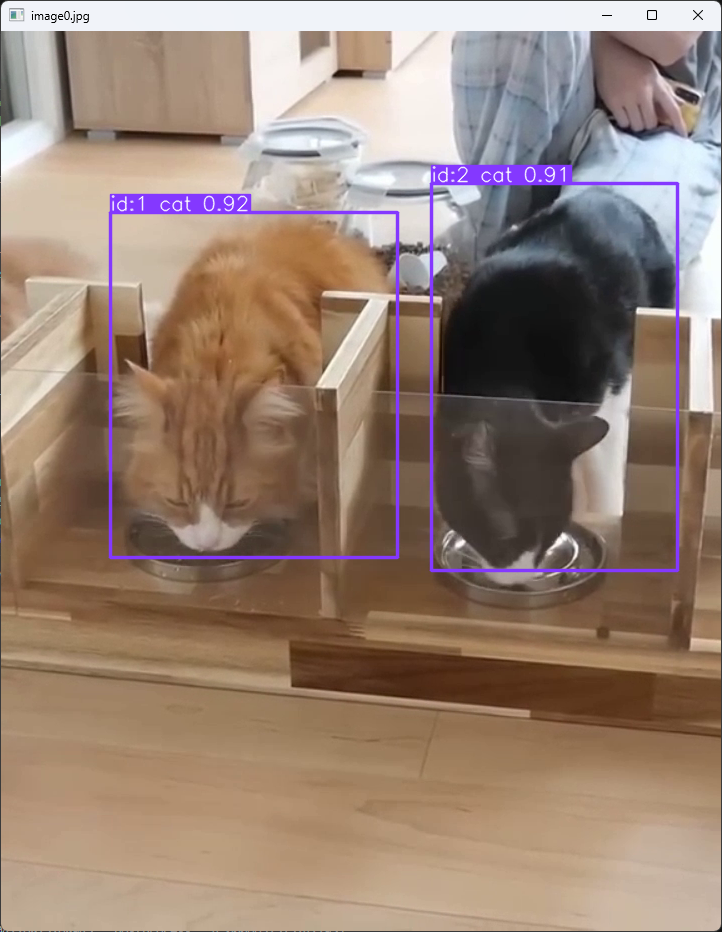
\includegraphics[width=0.35\textwidth]{img/AI/1.png}
\end{itemize}
\begin{itemize}
    \subitem It runs through the footage of cat drinking water using OpenCV. If cat is present, pretrained YOLOv8 model will detect and crop the cat from frame of the footage. YOLOv8 offers save\_text function which will make an txt file containing class(cat=15), annotation, and id information of cropped cats. Rest of the Python script will turn the txt file into Pandas DataFrame and will be used to store captured cats' information. \\
\end{itemize}

\subsubsection{Cat Color Detection}
\begin{itemize}
    \subitem The Python script employs computer vision and machine learning techniques to analyze images of cats, extracting dominant color information. The Ultralytics YOLO model is first used for object detection and segmentation, isolating cat-related objects in the images. The script then applies K-Means clustering to identify five dominant colors in each segmented image, calculating their frequencies. The dominant color and its associated name are determined, and the color information is integrated into a DataFrame representing cat-related attributes. Additionally, the CIELAB color space is utilized to enhance color representation. The script incorporates functions to handle color similarity, conversion between different color representations, and updates the DataFrame with the extracted color information. Finally, the script saves the processed DataFrame, including dominant color and CIELAB color, back to the original CSV file that contains the image labels and identifiers. \\
\end{itemize}

\subsubsection{Cat Breed Detection}
\begin{itemize}
    \subitem The Python script utilizes a pretrained(custom) ResNet-50 model for image classification on a dataset containing images of cats. The model, loaded with weights, is fine-tuned on the specific task of identifying cat breeds using transfer learning. A custom model head is added to the ResNet-50 architecture, consisting of fully connected layers. The trained model is then used to predict the breed of cats in a set of images, and the results are integrated into a DataFrame representing cat-related attributes. The script incorporates image preprocessing steps, including resizing and normalization, before feeding them into the model. The predicted breed labels are then appended to the DataFrame, and the updated DataFrame is saved back to the original CSV file. The script is designed to handle multiple cat images and categorize them based on their predicted breeds, utilizing the ResNet-50 model's classification capabilities. \\
\end{itemize}

\newpage
\section{ARCHITECTURE DESIGN \& IMPLEMENTATION}
\subsection{Overall architecture}
\begin{itemize}
    \item[] 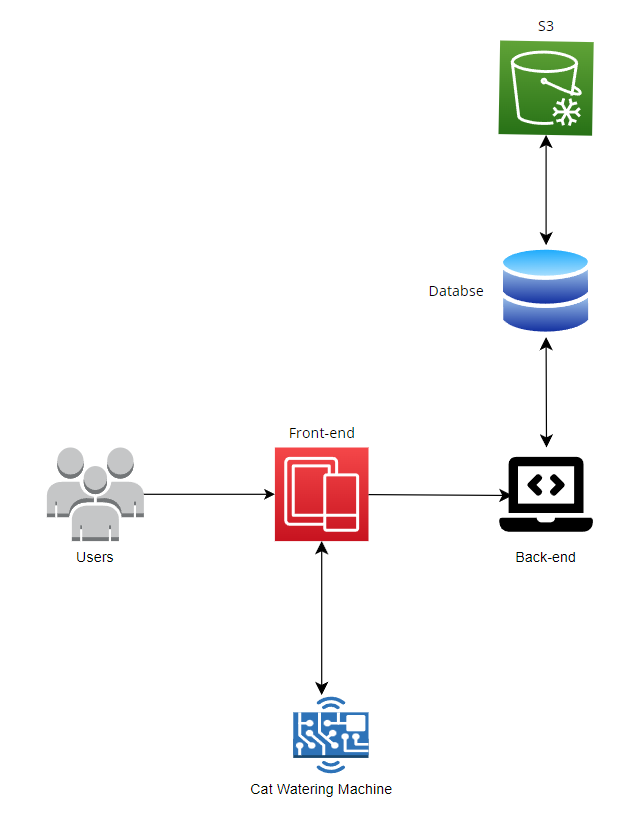
\includegraphics[width=0.4\textwidth]{img/Screen/architecture.png}
\end{itemize}
The overall architecture of our system is designed with several interconnected modules. Users interact with our application, and any input or information provided through the app is transmitted to the backend server via a REST API. The backend is a infrastructure that leverages MySQL for database management and AWS S3 for scalable storage solutions.\\

The user-facing application serves as the front end, allowing individuals to easily interact with the system. Behind the scenes, the REST API acts as a communication bridge between the application and the backend server. This ensures a standardized and secure method for transmitting data. On the hardware side, we have the CatFeeder module, which also communicates with the backend server through REST API.\\

MySQL serves as the relational database management system, providing a structured and organized storage solution for our data. AWS S3, on the other hand, handles object storage, offering scalability and durability for larger datasets and file storage needs.

\newpage
\subsection{Directory organization}
\begin{enumerate}
    \item FrontEnd
    \begin{flushleft}
        \tablefirsthead{\toprule Directory & File name \\ \midrule}
        \tablehead{\toprule Directory & File name \\ \midrule}
        \tabletail{\midrule }
        \tablelasttail{\bottomrule}
        \begin{supertabular}{p{0.42\linewidth} | p{0.5\linewidth}}
        /root & \makecell[l]{App.tsx}\\
        \midrule
        /src/api/common & \makecell[l]{autoLogin.ts\\messageAuth.ts\\checkMessageAuthCode.ts\\getUserProfile.ts}\\
        \midrule
        /src/api/localSignUp & \makecell[l]{checkEmailAvailable.ts\\localSignUp.ts}\\
        \midrule
        /src/api/login & \makecell[l]{login.ts}\\
        \midrule
        /src/api/find & \makecell[l]{checkUserExists.ts\\getFindEmail.ts\\sendPw.ts}\\
        \midrule
        /src/api/userProfileSet & \makecell[l]{registUserProfile.ts\\modifyUserProfile.ts}\\
        \midrule
        \makecell[l]{\small /src/api\\ \footnotesize/pendingCoManagerAddition} & \makecell[l]{getManagementSpaceId.ts}\\
        \midrule
        /src/api/catInfoSet & \makecell[l]{registCatInfo.ts}\\
        \midrule
        \makecell[l]{/src/api/catInfoSet\\/catProfileSet} & \makecell[l]{getCatProfile.ts\\modifyCatProfile.ts}\\
        \midrule
        \makecell[l]{/src/api/catInfoSet\\/catPhotosForAISet} & \makecell[l]{callAI.ts}\\
        \midrule
        \makecell[l]{/src/api/catInfoSet\\/catFeedStuffSet} & \makecell[l]{getCatFeedStuff.ts\\modifyCatFeedStuff.ts}\\
        \midrule
        \makecell[l]{/src/api/catInfoSet\\/catHydrationSet} & \makecell[l]{getCatHydration.ts\\modifyCatHydration.ts}\\
        \midrule
        /src/api/main & \makecell[l]{getCatProfileList.ts\\getCatMainInfo.ts}\\
        \midrule
        /src/api/drawer & \makecell[l]{deleteCatInfo.ts\\logout.ts}\\
        \midrule
        {\small /src/api/hydrationStatistics} & \makecell[l]{getCatStatistics.ts}\\
        \midrule
        /src/api/coManager & \makecell[l]{getManagerList.ts\\deleteCoManager.ts\\userSearch.ts\\addCoManager.ts}\\
        \midrule
        /src/components & \makecell[l]{AutoLoginCheckBox.tsx\\CatProfileList.tsx\\Loading.tsx\\ManagerCard.tsx\\TopBar.tsx}\\
        \midrule
        /src/components/button & \makecell[l]{ButtonUI.tsx\\ProcessButton.tsx\\SelectButton.tsx\\SignUpButton.tsx\\UnderlineTextButton.tsx}\\
        \midrule
        \makecell[l]{/src/components\\/inputContainer} & \makecell[l]{InputContainer.ts\\ImageInputContainer.tsx}\\
        \midrule
        /src/components/alert & \makecell[l]{Alert.tsx\\SearchUserAlert.tsx\\SelectCatAlert.tsx}\\
        \midrule
        /src/components/drawer & \makecell[l]{Drawer.tsx\\DrawerRoute.tsx\\SubDrawerRoute.tsx}\\
        \midrule
        /src/components/drawer & \makecell[l]{Drawer.tsx\\DrawerRoute.tsx\\SubDrawerRoute.tsx}\\
        \midrule
        /src/components/calendar & \makecell[l]{index.ts\\CalendarHeader.tsx\\WeekCalendar.tsx\\MonthCalendar.tsx\\YearCalendar.tsx}\\
        \midrule
        /src/components/graph & \makecell[l]{index.ts\\HydrationGraph.tsx\\XAndBar.tsx}\\
        \midrule
        /src/contexts & \makecell[l]{UserContext.tsx\\CatContext.tsx\\CatInfoContext.tsx}\\
        \midrule
        /src/data/common & \makecell[l]{
        checkMessageAuthCode\\FormType.ts}\\
        \midrule
        /src/data/localSignUp & \makecell[l]{
        \small localSignUpFormType.ts\\ \small requestMessageAuthFormType.ts}\\
        \midrule
        /src/data/login & \makecell[l]{
        loginFormType.ts}\\
        \midrule
        /src/data/find & \makecell[l]{
        findEmailFormType.ts\\findPwFormType.ts}\\
        \midrule
        /src/data/userProfileSet & \makecell[l]{
        userProfileFormType.ts}\\
        \midrule
        \makecell[l]{/src/data/catInfoSet\\catProfileSet} & \makecell[l]{\small catProfileSetFormType.ts}\\
        \midrule
        \makecell[l]{/src/data/catInfoSet\\catPhotosForAISet} & \makecell[l]{\small catPhotosForAISetFormType.ts}\\
        \midrule
        \makecell[l]{/src/data/catInfoSet\\catFeedStuffSet} & \makecell[l]{\small catFeedStuffSetFormType.ts}\\
        \midrule
        \makecell[l]{/src/data/catInfoSet\\catHydrationSet} & \makecell[l]{\small catHydrationSetFormType.ts}\\
        \midrule
        /src/hooks & \makecell[l]{
        useGoScreen.ts\\useLoading.ts}\\
        \midrule
        /src/nav & \makecell[l]{
        MainNavigator.tsx}\\
        \midrule
        /src/screens & \makecell[l]{
        Start.tsx\\Login.tsx}\\
        \midrule
        /src/screens/localSignUp & \makecell[l]{
        index.ts\\BasicForm.tsx\\RequestMessageAuth.tsx\\CheckMessageAuthCode.tsx}\\
        \midrule
        /src/screens/find & \makecell[l]{index.ts\\FindEmail.tsx\\FindEmailResult.tsx\\FindPw.tsx\\CheckMessageAuthCode.tsx}\\
        \midrule
        \makecell[l]{/src/screens\\/userProfileSet} & \makecell[l]{index.ts\\UserProfileSet.tsx\\UserProfileRegistration.tsx\\UserProfileModification.tsx}\\
        \midrule
        \makecell[l]{/src/screens\\/prepareSpace} & \makecell[l]{index.ts\\HowToGoSpace.tsx\\DeviceRegistration.tsx\\ \small PendingCoManagerAddition.tsx}\\
        \midrule
        \makecell[l]{/src/screens\\/catInfoSet\\/catProfileSet} & \makecell[l]{index.ts\\CatProfileSet.tsx\\CatProfileRegistration.tsx\\ CatProfileModifiation.tsx}\\
        \midrule
        \makecell[l]{/src/screens\\/catInfoSet\\/catPhotosForAISet} & \makecell[l]{index.ts\\CatPhotosForAISet.tsx\\ \small CatPhotosForAIRegistration.tsx\\AIResult.tsx}\\
        \midrule
        \makecell[l]{/src/screens\\/catInfoSet\\/catFeedStuffSet} & \makecell[l]{index.ts\\CatFeedStuffSet.tsx\\CatFeedStuffRegistration.tsx\\ CatFeedStuffModifiation.tsx}\\
        \midrule
        \makecell[l]{/src/screens\\/catInfoSet\\/catHydrationSet} & \makecell[l]{index.ts\\CatHydrationSet.tsx\\CatHydrationRegistration.tsx\\ CatHydrationModifiation.tsx}\\
        \midrule
        \makecell[l]{/src/screens/main} & \makecell[l]{index.ts\\Main.tsx\\HydrationStatistics.tsx\\CoManager.tsx}\\
        \midrule
        /src/styles & \makecell[l]{
        alertBackgroundStyles.ts\\mainView.ts}\\
        \midrule
        /src/utils & \makecell[l]{
        changeDateToString.ts\\checkCanPress.ts\\checkValid.ts\\localUriToFormData.ts}\\
        \midrule
        \end{supertabular}
    \end{flushleft}
    \vspace{0.5cm}

    \newpage
    \item BackEnd
    \begin{flushleft}
        \tablefirsthead{\toprule Directory & File name \\ \midrule}
        \tablehead{\toprule Directory & File name \\ \midrule}
        \tabletail{\midrule }
        \tablelasttail{\bottomrule}
        \begin{supertabular}{p{0.42\linewidth} | p{0.5\linewidth}}
        /API/ & \makecell[l]{addCoManager.js \\ autoLoginCase1.js \\ autoLoginCase2.js \\ checkEmailAvailable.js \\ checkMessageAuthCode.js \\ checkUserExists.js \\ deleteCatInfo.js \\ deleteCoManager.js \\ getCatFeedStuff.js \\ getCatHydration.js \\ getCatMainInfo.js \\ getCatProfile.js \\ getCatProfileList.js \\ getCatStatistics.js \\getFindEmail.js \\  getManagementSpaceId.js \\getManagerList.js \\getUserProfile.js \\ localSignUp.js \\ login.js \\ logout.js \\  messageAuth.js \\ modifyCatFeedStuff.js \\ modifyCatHydration.js \\ modifyCatProfile.js \\ modifyUserProfile.js \\ package-lock.json \\ package.json \\ registCatInfo.js \\ registUserProfile.js \\ sendPw.js \\ serverless.yml \\ userSearch.js}\\
        \midrule
        \end{supertabular}
    \end{flushleft}
    \vspace{0.5cm}

    \item AI
    \begin{flushleft}
        \tablefirsthead{\toprule Directory & File name \\ \midrule}
        \tablehead{\toprule Directory & File name \\ \midrule}
        \tabletail{\midrule }
        \tablelasttail{\bottomrule}
        \begin{supertabular}{p{0.42\linewidth} | p{0.5\linewidth}}
        [Front-end /root]/AI/  & \makecell[l]{flask\_app.py\\model.py\\requirements.txt\\./models/resnet50.pth\\./models/yolov8m-seg.pt}\\
        \midrule
        /AI/ & \makecell[l]{Cat Analysis AI.ipynb\\readme\\requirements.txt\\yolov8m-seg.onnx\\yolov8m-seg.pt\\yolov8n-seg.pt}\\
        \midrule
        /AI/data/ & \makecell[l]{cat.mp4}\\
        \midrule
        /AI/img/ & \makecell[l]{out.png}\\
        \midrule
        /AI/img/predict/crops/ & \makecell[l]{cropped images}\\
        \midrule
        /AI/img/predict/labels/ & \makecell[l]{generated dataframes}\\
        \midrule
        /AI/Model Training/ & \makecell[l]{Model Training\\Demonstration.ipynb}\\
        \midrule
        /AI/Model Training/data/ & \makecell[l]{Abyssinian\\Bengal\\Birman\\Bombay\\British Shorthair\\Egyptian Mau\\Maine Coon\\Persian\\Ragdoll\\Russian Blue\\Siamese\\Sphynx}\\
        \midrule
        /AI/Model Training/images/ & \makecell[l]{train\\val\\test}\\
        \midrule
        /AI/Model Training/checkpoints/ & \makecell[l]{best\_checkpoint.pth\\epoch_n_checkpoint.pth}\\
        \midrule
        \end{supertabular}
    \end{flushleft}
    \vspace{0.5cm}
\end{enumerate}
\vspace{0.5cm}

\subsection{FrontEnd Module}

\subsubsection{Utils}

\begin{itemize}
    \item purpose and functionality : A module containing frequently used functions in various Screens, Components, and API modules
    \item location of module : src/utils
    \item modules in Utils module
    \begin{itemize}
        \item checkValid: Performs validation differently based on input types and returns the validation results
        \item checkCanPress: Verifies if validation has been successful and enables buttons accordingly.
        \item localUriToFormData: Converts uploaded image files from users into formData for uploading to S3
        \item changeDateToString: Converts Date objects to strings for date comparison since dates from the server are in string. format
        \vspace{0.5cm}
    \end{itemize}
\end{itemize}
\subsubsection{Data}
\begin{itemize}
    \item purpose and functionality : Modularized to specify the type and initial values of formData used in information entry and modification screens, enhancing code readability. It also includes validation results for each input value
    \item location of module : src/data
    \vspace{0.5cm}
\end{itemize}

\subsubsection{Hooks}

\begin{itemize}
    \item purpose and functionality : A module created for creating custom hooks that handle repetitive state management and side effects. These hooks are intended to be imported and used where necessary
    \item location of module : src/hooks
    \item modules in Hooks module
    \begin{itemize}
        \item useGoScreen : Navigation to the previous screen, specific screens, and sending parameters while navigating to a specific screen
        \item useLoading : Displays a loading indicator while waiting for API responses
        \vspace{0.5cm}
    \end{itemize}
\end{itemize}

\subsubsection{Contexts}

\begin{itemize}
    \item purpose and functionality : A module utilizing the Context API to provide globally managed states and setter functions needed across multiple screens through Providers
    \item location of module : src/contexts
    \item modules in Contexts module
    \begin{itemize}
        \item UserContext : Manages states such as 'isMainDataChanged' determining if the main screen needs re-rendering, 'userEmail' and 'managementSpaceId' required for data binding and API calls across multiple screens. Additionally, 'userPw', 'userName', and 'userPhoneNum' are used to retain information entered in previous screens during signup, email recovery, and password recovery. For security reasons, 'userPw', 'userName', and 'userPhoneNum' are immediately initialized.
        \item CatInfoContext : The registration of cat information involves passing through screens for profiles, AI photos, wet food input, and finally, the hydration input screen. The API call is triggered upon pressing the registration button on this last screen. Therefore, a state to retain cat information from the previous stages is necessary until hydration input.
        \item CatContext : The state includes the Id and profile picture for the profile list of cats managed within the space, utilized across the main screen, statistics screen, and cat selection alert.
        \vspace{0.5cm}
    \end{itemize}
\end{itemize}

\subsubsection{Components}

\begin{itemize}
    \item purpose and functionality : Modules designed to be used as common components across various screens or for complex components, enabling their customization and easy implementation wherever required.
    \item location of module : src/components
    \item modules in Components module
    \begin{itemize}
        \item TopBar : Appears on all screens and consists of a back button, screen title, and a button for opening/closing the drawer.
        \item inputContainer
        \begin{itemize}
            \item Text Input: Used on information input screens, validates input types and displays validation results below the input field if necessary.
            \item Image Input: Allows users to move to their gallery upon clicking a camera icon and displays the selected image.
        \end{itemize}
        \item button : A button to execute a particular logic, a button to choose between two options
        \item alert : A basic alert, an alert for selecting a cat when modifying/deleting cat information, and a user search alert for adding co-managers.
        \item CatProfileList : Lists profile pictures of cats managed within a space, allowing selection of a cat profile to view information.drawer : Displays the user profile at the top and includes buttons for modifying a user profile, registering a cat profile, modifying a cat profile, deleting a cat profile, adding co-managers, and logout.button : A button to execute a particular logic, a button to choose between two options
        \item drawer : Displays the user profile at the top and includes buttons for modifying a user profile, registering a cat profile, modifying a cat profile, deleting a cat profile, adding co-managers, and logout.
        \item calendar : Contains a header with left and right buttons for changing the period and different designs for weekly, monthly, and yearly.
        \item graph : Appears on the hydration statistics screen, where the width of bars varies based on the number of x-values.
        \item ManagerCard : A card displaying the profile picture and information of co-managers.
        \vspace{0.5cm}
    \end{itemize}
\end{itemize}

\subsubsection{Styles}

\begin{itemize}
    \item purpose and functionality : A StyleSheet module used across various screens and components as a common styling
    \item location of module : src/styles
    \item modules in Styles module
    \begin{itemize}
        \item mainViewStyles : Includes styles for setting marginTop, center alignment, and adjusting component height to device height
        \item alertBackgroundStyles : Positions the Alert on top of the existing screen in an absolute position. It defines Alert width, height, alignment, and sets the background color of the Alert to gray.
        \vspace{0.5cm}
    \end{itemize}
\end{itemize}

\subsubsection{API}

\begin{itemize}
    \item purpose and functionality : A module intended for use in functional components to import and utilize API call and handling functions as needed. It utilizes Axios to send API requests to the server and processes responses based on different conditions.
    \item location of module : src/api
    \item modules in API module
    \begin{itemize}
        \item common : Includes APIs required across multiple screens such as automatic login, requesting SMS authentication, checking SMS verification codes, and fetching user profile information.
        \item localSignUp : Validates if an email is available and handles user registration based on user input.
        \item login : Handles login based on user input.
        \item find : Searches for an email based on user input. For password recovery, checks if there's a registered user matching the input and, if confirmed, sends the password via email.
        \item userProfileSet : Handles registration and modification of user profiles.
        \item pendingCoManagerAddition : Wait until confirming that user is registered as a co-manager.
        \item catInfoSet: Register cat information to manage, get cat profile/wet feed/hydration, modify it.
        \item main : Get the ID and profile picture of the cat registered in the space, and import main information of the selected cat.
        \item Drawer : Deletes cat information and logout that is processed immediately without moving the screen in the drawer.
        \item hydrationStatistics : fetching period-by-period hydration statistics data for selected cats
        \item coManager : Get a list of co-manager, delete co-manager, search for and add users to add as co-manager.
        \vspace{0.5cm}
    \end{itemize}
\end{itemize}

\subsection{BackEnd Module}
\subsubsection{Node.js - Serverless}
    \begin{itemize}
        \item Purpose : The project, being relatively small in terms of required APIs and involving two backend developers with limited project development experience, led to many considerations regarding server management and modularization. During this collaboration, the developers discovered the AWS Lambda serverless service, realizing that deploying APIs using this service allows for API-specific management without the need for separate server maintenance. Given the need to quickly develop APIs and manage servers, using serverless to modularize APIs and deploy them to the cloud was deemed suitable for the project scale.
        \item Functionality : Deployment and management of individual API endpoints.
        \item Location of Source Code
        \begin{itemize}
            \item Local: \texttt{API/root}
            \item AWS Lambda: \texttt{MulMeokNyang-prod/root}
        \end{itemize}
        \item Class Components : \texttt{serverless.yml}\\The code was modularized in individual JS files using the \texttt{serverless-http} module. The modularized code was then collectively deployed using the \texttt{serverless.yml} file.
        \begin{lstlisting}[style=htmlcssjs]
//getFindEmail.js
const express = require("express");
const app = express();
const mysql = require("mysql2");
const cors = require("cors");
const serverless = require("serverless-http");
const dotenv = require("dotenv");

// API code...

module.exports = {
  getFindEmail: serverless(app),
};
\end{lstlisting}
\\

\begin{lstlisting}[style=htmlcssjs]
\\serverless.yml
service: MulMeokNyang
frameworkVersion: "3"

provider:
  name: aws
  runtime: nodejs18.x
  environment:
    RDS_HOST: ${.env:RDS_HOST}
    RDS_USER: ${.env:RDS_USER}
    RDS_DATABASE: ${.env:RDS_DATABASE}
    RDS_PASSWORD: ${.env:RDS_PASSWORD}
    S3_BUCKET_NAME: ${.env:S3_BUCKET_NAME}
  memorySize: 2048
  timeout: 15
  stage: prod
  region: ap-northeast-2
  iamRoleStatements:
    - Effect: Allow
      Action:
        - s3:*
      Resource: arn:aws:s3:::S3_BUCKET_NAME

functions:
  autoLoginCase1:
    handler: autoLoginCase1.autoLoginCase1 //handler.module
    events:
      - http:
          path: /autoLoginCase1
          method: post

 getFindEmail:
    handler: getFindEmail.getFindEmail //handler.module
    events:
      - http:
          path: /getFindEmail
          method: get
% and more
\end{lstlisting}
    \end{itemize}

\subsection{AI Module} \\
Following features are performed when invoked from front-end(by uploading 5 images, it requests via API). Then results are returned to Front-end in JSON format.\\
\subsubsection{Cat Detection and Cropping (YOLOv8)}
\begin{itemize}
    \item Purpose: To identify and crop images of cats from footage using the YOLOv8 model.
    \item Functionality: The YOLOv8 model performs object detection and segmentation, saving a text file containing class (cat=15), annotation, and ID information of the cropped cats.
    \item Source Code: From Ultralytics Documentation
    \item Class Components: YOLOv8 model, OpenCV for video processing.
    \item Usage Explanation: YOLOv8 is employed for its efficient real-time object detection capabilities, with the script leveraging its save\_text function to store information about detected cats.
    \vspace{0.5cm}
\end{itemize}

\subsubsection{Cat Color Detection}
\begin{itemize}
    \item Purpose: To analyze images of cats and extract dominant color information.
    \item Functionality: Uses YOLOv8 for object detection, applies K-Means clustering to identify dominant colors, calculates color frequencies, and utilizes the CIELAB color space for enhanced color representation.
    \item Source Code: Customized implementation in Python, utilizing OpenCV, PIL, and scikit-learn for image processing and color analysis.
    \item Class Components: Functions for color analysis, K-Means clustering, and DataFrame manipulation.
    \item Usage Explanation: The script enhances the cat-related information by extracting dominant color details, contributing to a more comprehensive DataFrame representing cat attributes.
    \vspace{0.5cm}
\end{itemize}

\subsubsection{Cat Breed Detection (ResNet-50)}
\begin{itemize}
    \item Purpose: To predict the breed of cats in a set of images.
    \item Functionality: Utilizes a pretrained ResNet-50 model fine-tuned for cat breed classification, integrates predicted breed labels into a DataFrame.
    \item Source Code: Customized implementation using PyTorch and torchvision for deep learning.
    \item Class Components: Custom model head, PyTorch functions for model training, DataFrame manipulation.
    \item Usage Explanation: Transfer learning is employed to leverage the knowledge encoded in the pretrained ResNet-50 model for cat breed classification, enhancing the script's ability to categorize cats based on their predicted breeds.
    \vspace{0.5cm}
\end{itemize}

\section{USE CASES}

\subsection{New User of the Application}

\subsubsection{Start}
\begin{itemize}
    \begin{itemize}
        \item Click the "Sign up by email" button to proceed with the registration.
        \vspace{0.3cm}
    \end{itemize}
\end{itemize}

\subsubsection{Sign Up}
\begin{itemize} 
    \begin{itemize}
        \item Enter email, password, and confirm the password for account information.
        \item If the email and password are validated, move to the next screen for name and phone number verification through SMS.
        \item Enter the 6-digit verification code received via SMS. If user clicks the 'complete' button, verify the code. After verifying, display an alert indicating successful registration and proceed to the login screen.
        \vspace{0.3cm}
    \end{itemize}
\end{itemize}

\subsubsection{Login}
\begin{itemize}
    \begin{itemize}
        \item Log in with the email and password entered during registration.
        \item 'Automatic Login' button is the function for users who completed the user profile registration. If not, display an alert, "Automatic Login is available after user profile registration." Then, move to user profile registration.
        \item If the user forgets the email, they can click on the 'Fine Email' button.
        \begin{itemize}
            \item Enter the name and phone number used during registration.
            \item If user enter incorrect information, an alert is displayed 'There are no users found.'
            \item On the next screen, user can check the email when user signed up for membership. After that, user can choose whether to login or find password.
        \end{itemize}
        \item If the user forgets the password, they can click on the "Find Password" button.
        \begin{itemize}
            \item Enter the email and phone number entered when registering as a member, and press the 'Do message authentication' button. 
            \item Enter 6 digits of the authentication number sent by SMS and press the 'complete' button. If the authentication number does not match, user can see an alert that says 'It does not match', and if it matches, user can see an alert that says 'The password was sent to the email'.
            \vspace{0.3cm}
        \end{itemize}
    \end{itemize}
\end{itemize}

\subsubsection{User Profile Registration}
\begin{itemize}
    \begin{itemize}
        \item Enter user's profile picture, nickname, and self-introduction(optional).
        \item Create a new management space for cats to press 'Create my own management space' button 
        \item If user wants to join an existing space, press 'Pending on co-manager addition' button.
        \begin{itemize}
            \item When the main manager of the space allows the user to access the space, it moves to the main screen that manages the space.
        \end{itemize}
        \item Connect the cat watering machine to management space. Upon confirmation, proceed to cat profile registration.
        \vspace{0.3cm}
    \end{itemize}
\end{itemize}

\subsubsection{Cat Profile Registration}
\begin{itemize}
    \begin{itemize}
        \item Enter cat's name, age, weight, and profile photo(optional).
        \item In order for the watering machine to recognize the cat, the user needs to perform AI analysis for classifying the breed and extracting characteristic colors of the cat. The user can upload 5 pictures of their cat. By clicking the camera icon, they can access their gallery and add photos one at a time. If a photo is uploaded mistakenly, it can be deleted by clicking the X icon on the top right  of the photo. Once all 5 photos are uploaded, pressing the AI analysis button starts the analysis. Upon completion of the AI analysis, the breed and characteristic colors of the cat will appear on the screen. If unsatisfied with the analysis, pressing the 'Previous' button allows for a new AI analysis using a different photo."
        \item Enter the presence or absence of wet feed intake periodically. When the user presses the 'Yes' button, they enter the daily intake and water content of the feed (optional). Press 'No' to move on.
        \item Set the daily goal hydration. When the user presses the 'automatically' button, the daily goal hydration is automatically calculated and entered in the input below. By pressing 'manually', the user can enter the desired target amount of water consumption quantity.
        \item Complete the registration. If the user wants to add another cat, proceed to additional registration.
        \vspace{0.3cm}
    \end{itemize}
\end{itemize}

\subsubsection{Main}
\begin{itemize}
    \begin{itemize}
        \item After registering the user profile and registering the cat profile, the user accesses the main screen when login on the first screen. On the main screen, user can see a brief profile of the selected cat, daily water intake, and advice messages.
        \item Click on "View period-based hydration statistics" to see the cat's hydration statistics screen.
        \item If a user clicks on a different cat's photo at the top, it will switch to the main for that cat.
        \vspace{0.3cm}
    \end{itemize}
\end{itemize}

\subsubsection{Cat Hydration Statistics}
\begin{itemize}
    \begin{itemize}
        \item View the cat's hydration statistics on a weekly, monthly, or yearly by clicking each buttons. You can specify a specific time by clicking the calendar icon.
        \item In weekly statistics, user can check daily goal hydration  achievement rate.
        \item In monthly statistics, user can check the weekly average of goal hydration achievement rate.
        \item In the annual statistics, user can check the monthly average of goal hydration achievement rate.
        \item If user touches a bar, user can see detailed figures.
        \item If a user clicks on a different cat's photo at the top, it will switch to the main for that cat.
        \vspace{0.3cm} 
    \end{itemize}
\end{itemize}

\subsubsection{Drawer}
\begin{itemize}
    \begin{itemize}
        \item Access the overall service through the menu icon in the top right.
        \item Modify user profile
            \begin{itemize}
                \item User can modify the profile picture(optional), nickname, and self-introduction(optional) to be used by the application. Press the 'complete' button to return to the main screen.
                \vspace{0.3cm}
            \end{itemize}
        \item Add a new cat
            \begin{itemize}
                \item Go to the screen where user want to add a new cat. User would perform the same process as when registering for a cat profile. When the addition is complete, it returns to the main screen.
                \vspace{0.3cm}
            \end{itemize}
        \item Modify Cat's information 
            \begin{itemize}
                \item User can modify a cat's profile, wet food, and daily goal hydration. Clicking on the desired information to modify shows an alert to select the cat's profile for modifying. Upon pressing the 'modify' button, it moves to the cat profile modification screen. Once the modification is complete, it returns to the main screen.
                \vspace{0.3cm}
            \end{itemize}
        \item Delete Cat's profile
            \begin{itemize}
                \item When pressing the delete button, an alert appears to select the cat's profile for deletion. Upon pressing the 'Delete' button, it returns to the main screen, confirming the deletion of the cat's information.
                \vspace{0.3cm}
            \end{itemize}
        \item Manage co-administrators.
            \begin{itemize}
                \item User can see a list of users who are managing my cat's space. It is divided into main manager and co-managers.
                \item If user press the 'Add Co-manager' button, an alert will appear where user can add an co-manager. User enters a nickname, then click the search icon. And the search results will appear below. If user presses 'add' button, an alert will appear indicating that an co-manager has been added.
                \item If a user clicks on the trash can icon located at the bottom right of the co-manager card, an alert appears, asking if the user wants to delete the manager. Selecting 'Yes' enables the deletion of the co-manager.
                \vspace{0.3cm}
            \end{itemize}
    \end{itemize}
\end{itemize}

\subsection{Users already using the application (With Automatic Login)}
\begin{itemize}
    \item The loading occurs on the start screen, and once the loading finishes, it automatically transitions to the main screen.
    \item Subsequently, the user follows the same steps as described in USE CASE 1.
\end{itemize}

\section{DISCUSSIONS}
\subsection{Ann Jukyung}
Reflecting on this project experience, where my main responsibilities included backend API development and preparing presentation materials, I encountered several challenges, particularly in the realm of backend development. Being my first foray into this area, everything from understanding and implementing libraries and modules to the nuances of code syntax was a steep learning curve.\\

The initial phase of the project was the most daunting. I had to quickly familiarize myself with various backend technologies, understand how different APIs interact, and grasp the essentials of server management. The challenge was not just in learning new concepts but in applying them practically. I often found myself struggling with debugging and optimizing the code, which was both time-consuming and, at times, frustrating. \\

One of the most significant challenges was ensuring efficient communication between the backend and frontend parts of our application. Aligning the data formats, handling requests and responses, and ensuring data security were areas where I had to invest considerable effort and research. \\

Moreover, preparing presentation materials while simultaneously handling the technical aspects was a task that required effective time management. Distilling complex backend processes into understandable segments for the presentation demanded a different skill set. I had to balance between being technically accurate and making the content accessible to non-technical stakeholders. \\

Despite these challenges, the experience was immensely educational. I learned not just about technical aspects but also about resilience, the importance of thorough research, and the value of patience and persistence. Moving forward, I intend to apply the knowledge and collaborative experience gained from this project to numerous future endeavors. The practical insights I've acquired, particularly in backend development and team dynamics, will be invaluable assets in my ongoing professional journey. I aim to continuously integrate and leverage these learnings in upcoming projects, enhancing my technical proficiency and teamwork skills incrementally over time. \\

\subsection{Choi Chansol}
In this team project, I was responsible for the front-end development using React Native. Although I had prior experience with several development projects, my skills were lacking. I had only worked on small personal projects multiple times. However, through this project, I managed to implement the basic structure of a commercial application. From user registration and login to our service's unique feature of managing hydration spaces, I successfully implemented various functionalities. It feels satisfying to produce a proper outcome for the first time.\\

Especially, creating a mobile app using React Native felt like a significant growth point for me. Previously, React didn't resonate with me, so I mainly developed using vanilla JavaScript. However, inspired by this project, I decided to delve into React Native, a choice favored by many front-end developers. At the beginning of the semester, I spent a month studying theory by purchasing a book and practicing code examples. From mid-October, I began the front-end development and completed it within a month and a half.\\

My primary focus in this development was on modularization. I modularized functions and components that seemed likely to be reused later. Initially, although the functionality was limited, I felt concerned as the folder structure became complex and the number of files increased. However, as I progressed, I realized the importance of modularization. For instance, our application had several input fields. I created a custom component called 'inputContainer', allowing the creation of appropriate input fields on various screens by passing different property values based on the screen. It took me an entire day just to implement this component. Consequently, even though it seemed like I hadn't achieved much that day, creating intricate components resulted in quickly completing screens that required input fields in just about an hour and a half. Also, our application had similar screens for either registering or editing information. Initially, I struggled to figure out an efficient structure for these screens. However, I achieved modularization by passing the 'method' property to identify whether it's a registration or editing screen. Thus, I could implement identical UI/UX designs but handle modifications differently by implementing different callback functions for registration and editing buttons. As I progressed, although the content to be developed became more challenging, the consistent focus on modularization allowed me to progress steadily without delay.\\

However, there were some regrets. This was my first substantial project using React Native, and time was limited. Therefore, when faced with challenging concepts, I opted for an easier route instead of delving deeper. Regrettably, I abandoned two things. Firstly, Redux - I used the Context API to manage global states instead of Redux, which is more suitable for complex global state management. Since Redux was the most challenging part for me, I was unsure if I could handle it within the given time frame. However, due to the considerable number of global variables in our application, the code efficiency was compromised. Secondly, the Drawer component - I couldn't comprehend how to perform nested navigation using the Stack Navigator and Drawer Navigator together. Consequently, I created the Drawer as a custom component, and to navigate using the Drawer, I added screens directly to the Stack Navigator. Although I chose to abandon these due to time constraints, I'm planning to overcome these shortcomings during this winter break by working on new toy-projects.\\

Collaborating with the backend wasn't without challenges. Our team had two backend developers who were completely new to backend development. I took the initiative to create backend development guidelines explaining which APIs to implement and the logic behind them. Development started in November, and assuming the APIs were implemented, I had to write code to call these APIs and bind data. Therefore, it was challenging to verify the accuracy of the code I had written. If even in real-world scenarios, frontend development sometimes initiates before API development, one should become familiar with verifying using mock data for the initial validation.\\

\subsection{Lee Yunsun}
In my role using Node.js with the Express framework, I took charge of developing backend APIs and overseeing code reviews, subsequently deploying them serverlessly on AWS. The initial foray into API development and AWS services proved challenging, marked by trial and error. Notably, grappling with reading environmental variables in the code and configuring AWS S3 permissions posed difficulties. Branch merges were hindered by version disparities in modules, prompting a shift towards individual API distributions to mitigate collisions, albeit not entirely successfully.\\ 

Navigating through package.json, I gleaned insights into the critical role of version management. Despite encountering challenges, tapping into AWS official documentation and collaborative problem-solving within the team proved instrumental. This project provided a holistic view of software development, encompassing service planning through to distribution, and underscored the significance of teamwork in resolving issues.\\

\subsection{Hong JunGgi}
In my role overseeing AI development, I feel sorry for our team members, recognizing the challenges we faced throughout the process. The realization of even minor mistakes, including typos, took me several days. Delving into the intricacies of pre-trained models was a time-consuming endeavor, requiring a substantial investment to comprehend their workings effectively, espeically YOLO models from ultralytics.\\

The training phase, on the other hand, proved comparatively straightforward. Thanks to the professor's guidance, the official PyTorch documentation offered comprehensive codes that facilitated a step-by-step understanding of the training process. Troubleshooting became manageable through resources like Stack Overflow, enabling us to address errors as they arose while awaiting the computer's autonomous execution.\\

Yet, the most formidable aspects of the development journey were encountered during implementation, feature engineering, and file organization. Navigating the complexities of connecting the AI components seamlessly with both the front-end and back-end systems presented additional challenges. Deploying the model online initially aimed at utilizing AWS Sagemaker, but due to a time constraint resulting from extensive focus on AI training and development, I couldn't allocate time to master AWS intricacies. This led to a minor financial setback of \$4.4, as I inadvertently left the Sagemaker instance active.\\

Despite this setback, we successfully pivoted to a local deployment using Flask. This experience highlighted the multifaceted nature of AI development, emphasizing the need for a holistic approach that encompasses not only training but also the integration and deployment phases.\\

As we approached the project deadline, a significant realization dawned upon us—we found ourselves increasingly reliant on ChatGPT, even evolving into adept prompt engineers within a short span. This reliance underscored the versatility and efficiency of utilizing language models like ChatGPT in the development process.\\

Furthermore, reflecting on the project experience, I recognized the need to explore AI development with Tensorflow in the future. This shift would facilitate seamless integration of AI models with JavaScript format, particularly beneficial for mobile applications in the front-end. Additionally, I acknowledged the importance of diversifying the dataset, suggesting that in future AI endeavors, I should experiment with a broader range of cat breeds, deliberately ignoring class imbalances to observe the impact on accuracy.\\

The project journey also underscored the significance of soft skills in the realm of software development. Understanding software life cycles, effective communication methods, the importance of documentation, individual responsibilities, and proficient project management all emerged as crucial components. As software developers, it became evident that meticulous consideration of these factors is imperative to navigate through the development process smoothly. Effective communication, in particular, plays a pivotal role in preventing miscommunication and misunderstandings.\\

A key takeaway from this experience is the necessity of collaborative efforts in group development projects. Solo endeavors can lead to inefficiencies and misunderstandings. Instead, fostering open communication, understanding everyone's requirements, and delineating individual tasks contribute to a cohesive and successful development process. It serves as a reminder that the synergy of skills and ideas within a team enhances the overall quality of the project.\\

Frankly, initially, the concept of teaching a computer to analyze images and accurately predict their content, particularly in terms of categorization, struck me as a rather audacious idea. At the time, it seemed almost implausible. Little did I realize that I was somewhat lagging behind the rapid advancements in the modern tech world, and what I perceived as an audacious concept was merely the tip of the iceberg.\\

Through this project, I've come to understand that the AI landscape is continuously evolving, with advancements far beyond what I initially perceived as impossible. The project not only broadened my technical expertise but also shed light on the importance of soft skills in navigating the complexities of the AI industry. It underscored the dynamic nature of technology and the ongoing need for individuals to adapt and stay abreast of the latest developments.\\

In essence, this project has been a catalyst for my personal growth, providing insights into the limitless possibilities within the AI industry. It has ignited a curiosity to delve deeper into the unexplored realms of artificial intelligence, recognizing that there is so much more to be discovered and leveraged for the betterment of the world.\\

\end{document}